\documentclass[11pt]{article}
\usepackage[T1]{fontenc}
\usepackage{lmodern}
\usepackage[margin=1.1in]{geometry}
\usepackage{amsmath,amssymb,amsthm,mathtools}
\usepackage{microtype}
\usepackage{enumitem}
\usepackage{booktabs,array}
\usepackage{xcolor}
\usepackage{tikz}
\usetikzlibrary{arrows.meta,calc,patterns,positioning}
\usepackage[hyphens]{url}
\usepackage[colorlinks=true,linkcolor=blue!45!black,citecolor=blue!45!black,urlcolor=blue!45!black]{hyperref}
\hypersetup{pdftitle={A Linear Clock for Random Walk on Tree-Weighted Planar Maps},pdfauthor={OpenAI}}

\newtheorem{theorem}{Theorem}[section]
\newtheorem{proposition}[theorem]{Proposition}
\newtheorem{lemma}[theorem]{Lemma}
\newtheorem{corollary}[theorem]{Corollary}
\theoremstyle{definition}
\newtheorem{definition}[theorem]{Definition}
\theoremstyle{remark}
\newtheorem{remark}[theorem]{Remark}
\numberwithin{equation}{section}

\newcommand{\R}{\mathbb R}
\newcommand{\C}{\mathbb C}
\newcommand{\Z}{\mathbb Z}
\newcommand{\N}{\mathbb N}
\newcommand{\E}{\mathbb E}
\renewcommand{\P}{\mathbb P}
\newcommand{\dd}{\mathrm d}
\newcommand{\1}{\mathbf 1}
\newcommand{\en}{\mathsf e}
\newcommand{\enstar}{\mathsf e^{*}}
\newcommand{\cE}{\mathcal E}
\newcommand{\cQ}{\mathcal Q}
\DeclareMathOperator{\EL}{EL}
\let\Cap\relax
\DeclareMathOperator{\Cap}{Cap}
\DeclareMathOperator{\supp}{supp}
\DeclareMathOperator{\diam}{diam}
\DeclareMathOperator{\dist}{dist}
\DeclareMathOperator{\vol}{vol}
\DeclareMathOperator{\osc}{osc}
\DeclareMathOperator{\Law}{Law}
\DeclareMathOperator{\Var}{Var}
\DeclareMathOperator{\Area}{Area}
\newcommand{\articleid}[1]{\begingroup\Urlmuskip=0mu plus 2mu\relax\nolinkurl{#1}\endgroup}
\setlist{topsep=4pt,itemsep=3pt,parsep=0pt}
\setlength{\emergencystretch}{2em}

\title{A Linear Clock for Random Walk\\on Tree-Weighted Planar Maps}
\author{OpenAI}
\date{October 5, 2026}

\begin{document}
\maketitle
\begin{abstract}
We prove that stationary random walk on a planar map sampled with weight
equal to its number of spanning trees converges to Liouville Brownian
motion on the unit-area $\sqrt2$-Liouville quantum sphere. The convergence
retains the conditional path law jointly with the measured metric space.
The walk chooses uniformly among all incident half-edges and starts from
the stationary degree measure. For total attempt rate one and the
continuum Dirichlet form with factor $1/2$, the time acceleration is exactly
the number of map edges. The result uses the companion contour and metric
limits for this same ensemble.
\end{abstract}

\tableofcontents
\section{Introduction}\label{sec:introduction}

A scaling limit for the metric and area of a random surface does not by
itself determine the motion of a particle on that surface. The electrical
conductances of the approximating graphs can change the limiting
diffusion, even when their measured metric spaces converge. A further
question is whether the time needed to see the continuum motion has a
single deterministic normalization.

We resolve this question for planar maps weighted by their numbers of
spanning trees. The geometric input is the metric-measure limit and the
contour reconstruction theory of \cite{MetricMaps}. We prove the additional
convergence of the conditional walk laws, with an exact linear clock.
The proof separates the identification of the electrical energy from the
control of the speed measure. This separation is useful because neither
part follows from metric-measure convergence alone.

\subsection{The model and the continuum process}

A rooted planar map is a finite connected graph embedded in the oriented
sphere, up to orientation-preserving homeomorphism, with a distinguished
oriented edge. Loops and multiple edges are allowed. For $n\ge1$, let
$(M_n,T_n)$ be uniform among rooted maps with $n$ edges decorated by one
of their spanning trees. Thus the marginal weight of $M_n$ is proportional
to its number of spanning trees; conditional on $M_n$, the tree $T_n$ is
uniform. Write $V_n$ for the vertex set and $d_n$ for graph distance using
all map edges, each of length one. Set
\begin{equation}\label{eq:degree-measure}
 \mu_n=\sum_{v\in V_n}\frac{\deg(v)}{2n}\,\delta_v,
\end{equation}
where each loop contributes two to the degree.

Conditional on the map, let $X^n$ start from $\mu_n$. At the times of an
independent rate-one Poisson process it chooses an incident half-edge
uniformly and moves to its other endpoint. Choosing a loop makes no
displacement. Its generator is
\begin{equation}\label{eq:walk-generator}
 (L_nf)(v)=\frac1{\deg(v)}
   \sum_{e\text{ a half-edge at }v}
       \bigl(f(\operatorname{other}(e))-f(v)\bigr).
\end{equation}
The measure $\mu_n$ is stationary and reversible for this walk.

Let $(S,h)$ be an ordinary unit-area $\sqrt2$-Liouville quantum sphere,
with its distinguished points forgotten. We use the ordinary fixed-area
sphere law of Duplantier, Miller, and Sheffield \cite{DMS}. Its quantum
area measure $\mu_h$ has total mass one. Write $D_h$ for its Liouville
quantum gravity metric in a fixed deterministic normalization. Identify
the underlying conformal sphere with the round sphere. The continuum
process $B^h$ is the conservative $\mu_h$-symmetric diffusion associated
with the closure on $L^2(\mu_h)$ of
\begin{equation}\label{eq:continuum-form}
 \cE_h(f,g)=\frac12\int_{S^2}
      \langle\nabla f,\nabla g\rangle_{\mathrm{round}}
                    \,\dd\vol_{\mathrm{round}},
 \qquad f,g\in C^\infty(S^2).
\end{equation}
The closed form uses quasi-continuous representatives. This is Liouville
Brownian motion, started with conditional law $\mu_h$; see
\cite{GRV,Berestycki} and the Dirichlet-form framework in \cite{FOT}.
Conformal invariance of the two-dimensional Dirichlet integral makes
\eqref{eq:continuum-form} independent of the conformal coordinate. Its
factor $1/2$ fixes the continuum clock.

For precision we fix the spatial normalization used throughout. For a
finite real random variable $Y$, let $m(Y)$ be the unique real solution
of $\E[\arctan(Y-m(Y))]=0$. Put
\begin{equation}\label{eq:spatial-normalization}
 \Delta_n=\max\{1,\diam(V_n,d_n)\},\qquad
 \Delta=\diam(S,D_h),\qquad
 a_n=\exp\{m(\log\Delta)-m(\log\Delta_n)\}.
\end{equation}
Both centers use unconditional laws, so $a_n$ is deterministic. We use
the geometric limit of \cite{MetricMaps} in the form
\begin{equation}\label{eq:metric-premise}
 a_n\longrightarrow0,
 \qquad (V_n,a_nd_n,\mu_n)
       \xrightarrow{\ d\ }(S,D_h,\mu_h)
 \quad\text{in Gromov--Hausdorff--Prokhorov topology}.
\end{equation}
The contour and topological results from that work needed in addition
to \eqref{eq:metric-premise} are stated in Section~\ref{sec:inputs}.

\subsection{Retaining the conditional path law}

Fix $T>0$. If $(K,d,\mu)$ is a compact metric probability space, let
$Q$ be a Borel probability measure on $D([0,T],K)$. We regard
$(K,d,\mu,Q)$ up to isometries transporting both measures. For two such
quadruples, define $\delta_T$ as the infimum over isometric embeddings
$i:K\to Z$ and $j:K'\to Z$ into a common complete separable metric space
of
\begin{equation}\label{eq:delta}
 \max\left\{
 d_H^Z(iK,jK'),\ d_P^Z(i_*\mu,j_*\mu'),\
 d_P^{D([0,T],Z)}(i_*Q,j_*Q')\right\}.
\end{equation}
Here $d_H$ and $d_P$ denote Hausdorff and Prokhorov distances. The last
term uses the Skorokhod $J_1$ topology: time changes are increasing
continuous bijections of $[0,T]$, and both their uniform time displacement
and the uniform spatial discrepancy tend to zero. Each of the three
distances may be truncated at one. An embedding acts on a path at every
time.

\begin{samepage}
\begin{theorem}[Linear clock and conditional laws]\label{thm:main}
For every finite $T>0$, define
\[
 Q_n^T=\Law\bigl((X^n_{nt})_{0\le t\le T}\mid M_n,T_n\bigr),
 \qquad
 Q_h^T=\Law\bigl((B^h_t)_{0\le t\le T}\mid h\bigr).
\]
With the spatial normalization \eqref{eq:spatial-normalization},
\[
 (V_n,a_nd_n,\mu_n,Q_n^T)
       \xrightarrow{\ d\ }(S,D_h,\mu_h,Q_h^T)
       \qquad\text{for }\delta_T,
\]
through all positive integers $n$. Thus the deterministic clock
multiplier for \eqref{eq:walk-generator} and \eqref{eq:continuum-form}
is $c=1$.
\end{theorem}
\end{samepage}

The random probability law is part of the state in Theorem~\ref{thm:main}.
For example, the same argument gives joint convergence of any fixed
number of conditionally independent stationary walks on the same map:
in a common embedding, the associated conditional joint laws are the
finite products of $Q_n^T$. Their weak convergence follows from that of
$Q_n^T$. This preserves information about the shared environment.

\subsection{Context and related work}
Mullin's enumeration of tree-rooted maps \cite{Mullin} gives the
combinatorial starting point: the selected spanning tree and its
complementary dual tree encode a map by a two-coordinate walk. The
continuum counterpart is the mating-of-trees construction of
Duplantier, Miller, and Sheffield \cite{DMS}. At $\gamma=\sqrt2$ its
boundary-length coordinates are independent Brownian motions. Miller
and Sheffield \cite{MSSphere} give the corresponding finite-area
sphere description, and their imaginary-geometry construction
\cite{IG4} supplies the space-filling $\mathrm{SLE}_8$ between the two
continuum trees. Couplings of discrete and continuum encodings have
also been used to compare graph distances across random-map models
\cite{GHS}. The continuum metric itself is characterized in
\cite{GMMetric}, with conformal covariance established in
\cite{GMConformal}.

Liouville Brownian motion was constructed by Garban, Rhodes, and Vargas
\cite{GRV} and independently by Berestycki \cite{Berestycki} through a
change of Brownian time determined by quantum area. Its Dirichlet-form
description \cite{GRVForm} separates two structures: the energy is
conformally invariant, while the speed measure is quantum area. This
distinction explains why the clock is a separate part of a random-map
scaling limit.

Several works establish important parts of the discrete picture.
Gwynne, Miller, and Sheffield prove convergence of the Tutte embedding
of mated-CRT maps, including conditional walk-law convergence modulo
time parameterization \cite{GMS}. Their estimates for harmonic
functions compare discrete and continuum energies up to constants and control
oscillation \cite{GMSHarmonic}; their invariance principle for ergodic
scale-free environments develops a broader framework for embedded
networks \cite{GMS2}. Gwynne and Miller obtain resistance,
return-probability, and displacement estimates for several infinite
random planar maps, including spanning-tree-weighted maps \cite{GM}.

Berestycki and Gwynne prove parameterized, quenched convergence to
Liouville Brownian motion for mated-CRT maps \cite{BG}. Their
deterministic time scale is an annealed exit-time median, comparable
to the inverse quantum area of a cell. Whether its ratio to that
inverse area converges is left open in \cite[Remark~1.3]{BG}.
Theorem~\ref{thm:main} concerns
the finite combinatorial tree-weighted map and its stationary
half-edge walk. It retains the conditional path law together with
metric and area, and identifies the acceleration as exactly $n$
for \eqref{eq:continuum-form}.

Our geometric inputs are the companion results in \cite{MetricMaps}.
The nondegeneration argument adapts the local-flow method in
\cite[Section~``The canonical conformal structure'']{ConformalMaps}
to a primal and a dual electrical network. The use of planar duality
to determine an effective conductivity has classical precedents,
including Dykhne's exact-conductivity argument \cite{Dykhne}. Here
we must first construct the energy limit without regularity
assumptions on the shapes of discrete faces. A separate Green
estimate in the original finite-map law then controls sources of
small stationary mass and supplies the missing clock information.


\subsection{Proof strategy and reusable estimates}

For a finite graph embedded in the sphere, write
\begin{equation}\label{eq:network-energy}
 \en(u)=\sum_{ab\in E}(u(a)-u(b))^2,
\end{equation}
with one term for each unoriented edge, including multiplicities. Loops
contribute zero. The same convention defines $\enstar$ on the dual graph.
The two main tasks are to identify the limit of these unnormalized
energies and to pass from that limit to motion in actual time.

The contour description of the map gives local finite graph pieces in
conformal coordinates. Section~\ref{sec:inputs} explains why the local
reconstruction and conditional-kernel calculations of \cite{MetricMaps}
also apply to extremal lengths and constrained energy minima on these
pieces. Exact edge incidences matter here: approximation of graph
distances alone would not identify an energy. The extension retains
compact numerical outputs before extracting a subsequence, and uses a
change of measure depending only on the contour inputs.

Section~\ref{sec:nondegeneration} proves bounded-energy cutoff estimates
without geometric control of individual faces. Its central argument is
a planar obstruction to simultaneous degeneracy of the primal and dual
networks. If annular extremal lengths could vanish, low-energy flows
would have a nonzero limiting average length measure. Locality and
triviality of field point germs produce transverse primal and dual
crossing flows at a typical point. Every such pair crosses an edge and
its dual, contradicting the vanishing traffic norms. The cutoffs then
yield harmonic compactness.

Section~\ref{sec:energy} identifies every local variational limit as
$\lambda\int|\nabla u|^2$, with the same positive deterministic $\lambda$
for the primal and dual. To determine $\lambda$, we compare a condenser
on an annulus with the period of its rotated current. The comparison in
one direction gives $\lambda\le1$; recovery of an angular cochain and
the signed primal--dual pairing give $\lambda\ge1$. Thus the coefficient
is exactly one in every subsequence. Section~\ref{sec:sphere} transfers
the result to fixed-area spheres using interior excursion densities and
removes the single omitted contour endpoint by zero Sobolev capacity.

The remaining speed-measure issue is addressed by the following estimate,
proved in Section~\ref{sec:green}. Let $H_n$ be the positive unweighted
graph Laplacian. For $\mu_n(f)=0$, define $G_nf$ by
$H_nG_nf=\mu_nf$ and $\mu_n(G_nf)=0$, where the product $\mu_nf$ on the
right denotes its vector of vertex masses. For every $0<\rho<1/2$ there
are map-measurable random variables $A_n$ with
$\sup_n\E A_n<\infty$ such that, simultaneously for $\|f\|_\infty\le1$,
\begin{equation}\label{eq:intro-green}
 \|G_nf\|_\infty\le A_n\,\mu_n(|f|)^\rho.
\end{equation}
Its proof is entirely in the fixed-size map law. A spanning-forest
identity expresses the centered inverse Laplacian through tree cuts;
the contour bijection expresses each cut size as one plus a dual-tree
distance. Dyck-excursion estimates then control the interval sums.
This estimate can be used independently of the energy identification.

Finally, Section~\ref{sec:dynamics} uses \eqref{eq:intro-green} to obtain
uniform resolvent convergence and a stopping-time tightness estimate.
The resolvents identify the conditional path laws by their integrated
finite-dimensional distributions. The normalization is visible already
at the discrete level:
\[
 -\langle f,nL_nf\rangle_{L^2(\mu_n)}=\tfrac12\en(f).
\]
Combining this identity with the coefficient $\lambda=1$ gives the clock
in Theorem~\ref{thm:main}.

\section{Sewing and local electrical observations}
\label{sec:inputs}

Electrical energy depends on every edge, including parallel edges.
Consequently, a description that approximates graph distances does not
by itself suffice for our purpose.  This section explains how the local
sewing construction of \cite{MetricMaps} retains exact graph pieces and
gives conditional laws for numerical observations on those pieces.
The observations may be extremal lengths or constrained energy minima;
we do not yet assert that they are bounded or identify their limits.
The construction has three parts.  We recover complete finite graph
pieces from contour cells, pass their numerical observations to
conditional limiting laws, and then read those laws from the fields
in the corresponding spatial regions.

Throughout this section,
\[
 \gamma=\sqrt2,\qquad Q=\frac2\gamma+\frac\gamma2=\frac3{\sqrt2},
 \qquad \chi=\frac1{\sqrt2}.
\]
All quantum surfaces use the field and boundary-length normalizations of
\cite{MetricMaps}.  A compact containment $K\Subset U$ means that $K$ is
compact and contained in the open coordinate domain $U$.  A buffer for
$K$ is an open neighborhood whose closure is compactly contained in $U$.

\subsection{The discrete graph and its continuum background}

Let $Z^{\mathrm d}=(L^{\mathrm d},R^{\mathrm d})$ be a bilateral walk
whose increments are independent and uniform on the four axial unit
vectors.  For integer times $i\le j$, set
\begin{equation}\label{inp:vertex-equivalence}
 i\sim_L j
 \quad\Longleftrightarrow\quad
 L^{\mathrm d}_i=L^{\mathrm d}_j
       =\min_{i\le k\le j}L^{\mathrm d}_k.
\end{equation}
The equivalence classes are the primal vertices.  Horizontal steps give
tree edges between consecutive classes, with the two traversals of a
tree edge counted as one edge.  A vertical up-step ending at $u$ and
the vertical down-step ending at $v>u$ are matched when
\begin{equation}\label{inp:step-match}
 R^{\mathrm d}_{u-1}=R^{\mathrm d}_v
      <\min_{u\le k<v}R^{\mathrm d}_k.
\end{equation}
Each matched pair contributes one further edge between $[u-1]_L$ and
$[v-1]_L$.  Distinct matched pairs remain distinct edges when their
endpoints agree.  In particular loops and parallel edges are retained.
Interchanging $L^{\mathrm d}$ and $R^{\mathrm d}$ gives the dual graph
and its complementary spanning tree.

For a finite interval of indices, the \emph{internal graph} uses the
same vertex relation, all horizontal steps in that interval, and the
vertical pairs whose two occurrences lie in the interval.  Its vertices
embed injectively into the full graph: the minimum test between two
retained times is the same in both constructions.  It need not contain
every full-graph edge between those vertices.

\begin{proposition}[Sewing and continuum background]\label{inp:sewing}
The following couplings and normalizations will be used.
\begin{enumerate}
\item A uniform rooted map--spanning-tree pair with $n$ edges is encoded
by the axial walk conditioned to remain in $\mathbb Z_{\ge0}^2$ and
return to zero after $2n$ steps.  The preceding rules recover every
primal and dual edge with its incidences.
\item Give the bilateral walk an independent Poisson clock of rate
$m$ and multiply its heights by $m^{-1/2}$.  As $m\to\infty$, its
interpolated contour converges locally uniformly in distribution to
$Z=(L,R)$, whose independent Brownian coordinates have variance
$1/2$ per unit time.  The limiting contour has the peanosphere coupling
with a $\sqrt2$-quantum cone $h$ and an independent whole-plane
space-filling $\mathrm{SLE}_8$, subsequently parameterized by $\mu_h$.
Write this curve as $\eta$ and normalize $\eta(0)=0$.
\item The imaginary field $\widehat h$ is independent of $h$ and is a
whole-plane GFF modulo $2\pi\chi\mathbb Z$, with uniform phase in
one period.  It determines the oriented curve before area
parameterization.  The fields, curve, and contour are retained with
their joint peanosphere law.
\item A finite interval of contour increments determines its abstract
decorated quantum surface, its restricted curve, and the quantum lengths
of its incoming and outgoing frontiers, modulo conformal coordinates.
The analogous statement holds for every symmetric interior interval
of the Brownian-excursion encoding of the ordinary unit-area sphere.
\end{enumerate}
\end{proposition}

The discrete assertion is Mullin's encoding \cite{Mullin}, in the form
of Theorem ``Mullin encoding and its infinite version'' in
\cite{MetricMaps}.  The continuum assertions are recorded in its
Theorem ``Peanosphere and interval surfaces'' and its imaginary-field
normalization.  Their principal continuum inputs are the mating of
trees theorems of \cite[Theorems~1.9 and~1.11]{DMS} and the
space-filling construction of \cite{IG4}.
The use of a Poisson clock makes the two coordinate jump processes
independent; index time divided by $m$ has the same limiting area time.

We recall the geometric information accompanying this coupling.  Two
continuum times have the same image under $\eta$ precisely when they
are equivalent under the relation generated by
\begin{equation}\label{inp:brownian-fibers}
 L_s=L_t=\inf_{[s,t]}L
 \quad\hbox{or}\quad
 R_s=R_t=\inf_{[s,t]}R,\qquad s\le t.
\end{equation}
Except for the common endpoint in the sphere encoding, every class has
at most three elements and belongs to one coordinate when it is
nonsingleton.  In a class $t_1<t_2<t_3$, the middle time is a strict
local minimum; distinct strict local minima have different heights.
At parameter $8$, the interval cells are closed topological disks.
The cone curve is proper, so inverse images of compact sets are bounded.
These facts, including their simultaneous versions on a countable
collection of intervals and independent Poisson cuts, are the
topological input accompanying Theorem ``Peanosphere and interval surfaces'' of
\cite{MetricMaps}; see also the identification description in
\cite[Section~1.3.1 and Lemma~8.15]{DMS}.

All subsequential arguments below can be placed in a coupling with
locally uniform contour convergence.  We attach the full continuum
background conditionally on the limiting contour, independently of
the additional \emph{raw} discrete observations given that contour.
Here raw means that the observation uses contour labels, without
projecting them through $\eta$.  This convention is compatible with
further extraction.  Indeed, for a bounded background test $F$, its
conditional expectation $k_F(Z)$ can be approximated in $L^1$ of the
fixed Brownian marginal by bounded continuous functions of $Z$.
Multiplying by any bounded raw test leaves the approximation error
uniformly bounded by the same $L^1$ error.  Joint weak convergence
therefore preserves the conditional sampling identity.  Spatially
projected observations will depend on both the raw data and the
background; we only make this conditional sampling assertion before
projection.

\subsection{Projections and planar topology}

Regard the map together with its dual as a cell decomposition of a
surface, subdivided into triangles at its corners.  Assign a primal or
dual vertex the point $\eta(t)$ corresponding to any of its visits.
All choices at one vertex, and all corners of an incident triangle,
have uniformly vanishing discrepancy.  Otherwise a subsequence of
visit times would limit to a discrete equality or matching relation
whose endpoints have distinct continuum images, contradicting
\eqref{inp:brownian-fibers}.  Join nearby assigned points by short
coordinate arcs and fill the triangles in small disks.  This gives
continuous projections $\pi_m$ with vanishing projected triangle mesh.
On the plane this construction is made in a bounded window containing
the region under consideration, after preserving its necessary stars
and capping the window.  This protection is obtained directly from
lower contour visits, as in the proof below; it does not use a local
instruction graph or any numerical-array limit.

\begin{proposition}[Topological comparison]\label{inp:topology}
In the contour coupling, the projections $\pi_m$ may be chosen so that
the following conclusions hold on the sphere and on every buffered
compact part of the plane.  Each conclusion is eventual for each
fixed choice of margins.
\begin{enumerate}
\item If the projections of two primal vertices approach each other,
they can be joined by primal paths with arbitrarily small projected
diameter.  This is uniform over all lifts in a fixed compact region.
The same statement holds on the dual graph and for surface paths.
In particular fixed tubes with clearance contain paths following them
on either graph.
\item All lifts of a sufficiently small closed disk or other compact
well can be included in a connected set over any fixed open
enlargement.  A loop projecting into a small disk can be filled over
a slightly larger disk, provided that both have the prescribed
clearance.
\item The projection has degree $+1$ or $-1$ in a compact spherical
completion.  Robustly transverse primal and dual tube crossings
intersect at an edge and its dual.  Projected circuits with nonzero
winding difference about two separated wells separate all the
corresponding lifted fibers.
\item Integer winding differences about two wells agree upstairs and
downstairs up to the common degree sign, when loops and wells have
fixed separation.  These statements retain repeated edge and face
incidences.
\end{enumerate}
\end{proposition}

\begin{proof}
The construction and the first three assertions are the construction
preceding Lemma ``Uniform topological joining'', that lemma,
Lemma ``Exterior connection and small-loop filling'', Proposition
``Degree and robust planar topology'', and Lemma ``Separation of
entire fibers'' in \cite{MetricMaps}.
We explain their applicability to both graphs and to the plane.

The hypotheses are uniform contour convergence, vanishing projected
cell mesh, and approximation of the limiting fiber generators by
discrete links with small projected connecting paths.  For a Brownian
excursion above a level, use last and first crossings of nearby levels
on the two sides of an interior time.  Their discrete analogues
approximate the chord.  At a triple, apply this on the two excursions
on either side of its middle minimum.  The fiber description above
therefore supplies every generator required for topological joining.
Interchanging the coordinates gives the same argument for the dual.
Applying planar separation to the two embedded graph paths gives the
mixed crossing assertion: a primal path and a dual path can meet only
through a primal edge and its dual, with the usual corner subdivision
making the intersection literal on the surface.

For a bounded plane region, choose a window containing all its visits
and its fixed additional star layers.  Both contour coordinates make
strictly lower visits on both sides of a sufficiently large window.
Lemma ``Protected capping of a bounded window'' in
\cite{MetricMaps} then supplies a spherical completion preserving
all these incidences.  Its continuum completion is absolutely
continuous with respect to a Brownian excursion, which supplies the
sphere quotient needed for the preceding topological results.

For the integer assertion, connect all lifts of each well away from
the tested loop, using the first two assertions.  A two-chain bounded
by that loop has constant multiplicity along each such connected
fiber.  Projection multiplies the difference of its multiplicities
at the two fibers by $\deg\pi_m=\pm1$.  This is exactly the equality
of winding differences.  Equivalently, one can use relative homology
after a simplicial perturbation inside the fixed margins.
\end{proof}

\subsection{Finite instruction graphs and numerical tests}

For a finite multigraph $G$, write
\begin{equation}\label{inp:graph-energy}
 \en_G(u)=\sum_{ab\in E(G)}(u(a)-u(b))^2.
\end{equation}
The sum has one term for each unoriented edge; loops contribute zero.
An energy test is the infimum of \eqref{inp:graph-energy} subject to
finitely specified value constraints at vertices of a specified
subgraph.  We allow $+\infty$ for an infeasible test.  An extremal-length
test for a family $\mathcal P$ of graph paths is
\begin{equation}\label{inp:el-test}
 \EL_G(\mathcal P)=
 \sup_{w:E(G)\to[0,\infty)}
 \frac{\bigl(\inf_{P\in\mathcal P}\sum_{e\in P}w(e)\bigr)^2}
      {\sum_{e\in E(G)}w(e)^2},
\end{equation}
with the usual conventions for empty families and constant paths.
Only nontrivial families will be used in the crossing arguments.

The graph on which one computes these quantities must be specified
before taking a limit.  We use the finite instruction graphs of
Lemma ``Finite-band reconstruction'' in \cite{MetricMaps}, recalled next.
Their inputs consist of finite strings and relative heights.  This
description will also show why the conditional-law proof applies to
our numerical tests.

\begin{definition}[Finite packages]\label{inp:packages}
A \emph{master block} consists of two increment strings on a time
interval $[0,\ell_b]$, starting at zero, together with a finite list
of internal cuts.  A finite package contains finitely many master
blocks.  For each coordinate $a\in\{L,R\}$ choose a forest on these
blocks and record its height differences
$o^a_{bd}=s^a_d-s^a_b$.  The values $s^a_b$ are thereby determined
within each forest component up to one additive constant.

A test chooses finitely many \emph{active windows}, each between
recorded cuts of a master block.  Each active window initially has its
own copy of the contour vertices.  Its starting heights and increment
strings are obtained by restriction of its master block.  Enable the
ordinary sewing inside each active window.  The additional
cross-window links are specified by the band rules below.  A package
can retain several tests on the same master strings.
\end{definition}

For an active window $b$, write $z^a_b$ for its increment string,
$s^a_b$ for its starting height, and $m^a_b=\min z^a_b$.
Its incoming and outgoing record arcs are the times satisfying,
respectively,
\[
 z^a_b(t)=\min_{0\le u\le t}z^a_b(u),
 \qquad
 z^a_b(t)=\min_{t\le u\le\ell_b}z^a_b(u).
\]
A band from window $b$ to window $d$ permits outgoing-to-incoming
links with common absolute height $H$ satisfying
\begin{equation}\label{inp:bands}
 \alpha\le H-q\le\beta,
 \qquad H\le s^a_w+\min_J z^a_w\quad(w,J\text{ in the cap list}).
\end{equation}
Here $\alpha<\beta$ are fixed rational parameters, $q$ is the height
at a recorded anchor cut, and each $J$ is a recorded subwindow.
The forest supplies every relative height appearing in the rule.
Each selected minimum is evaluated from the discrete string itself.

In the primal graph, an $L$-band identifies its permitted vertices.
An $R$-band is a rule for pairs of oriented step occurrences: an
outgoing up-step and an incoming down-step must carry the same unit
height strip, and the \emph{whole strip} must satisfy the band and cap
conditions.  Such a pair contributes an edge; it does not impose an
$R$-vertex identification.  The dual uses the exchanged convention.
If a tree edge is represented in several retained pieces it is counted
once after the corresponding vertex identifications: its unordered
endpoint pair identifies it, since a tree has no parallel edges.
Each additional matched-step edge is counted once for that matched
pair, even when another such pair has the same endpoints.

The same active windows and band instructions continue to define an
old test when cuts are added or master blocks are merged.  In the
merged string, old starting heights are evaluated at the old cuts;
they are no longer independent offset parameters.  A graph allowed
to use the entire merged interval is a separate new test.  In
particular an old test cannot be recovered by merely confining paths
in that larger graph, since the larger graph may use newly enabled
edges witnessed in a formerly omitted gap.

For each instruction list we retain a countable family of numerical
outputs.  A vertex is selected when one of its visits lies in a finite
union of intervals of relative time.  Endpoints can be recorded cuts
or rational fractions between cuts.  Such selectors specify the
subgraph, its ports, and any confinement condition.  Rational value
intervals at selected visits specify energy constraints; repeated
visits impose simultaneous constraints on the same vertex.  The
output library includes both graphs, finite joint lists of tests,
and tests recomputed on union graphs.  Inapplicable tests receive a
fixed default value.  Every nonnegative output is compactified in
$[0,\infty]$, for example by $x\mapsto x/(1+x)$.
We can retain outputs divided by any prescribed positive deterministic
factor $b_m$, including factors tending to zero.

This gives compact countable products of numerical observations.  The
master strings, durations, cuts, and offsets remain separate input
coordinates.  Along any sequence $m\to\infty$, one may therefore
extract joint limits of all the raw tests and the locally convergent
contours.  The issue is now to relate these formal tests to complete
pieces of the actual map.

\subsection{Exact cores and the selector sandwich}

Add independent Poisson cuts in area time, using nested refinements.
A cell is the image of a consecutive cut interval under $\eta$.
Only cells compactly contained in the current testing domain will be
used.  Their local data consist of their oriented traversals, quantum
area parameterizations, and tagged incoming and outgoing frontier
lengths, with repeated frontier occurrences retained.
A \emph{run} is a finite union of consecutive cells, viewed with its
concatenated traversal and tagged incoming and outgoing frontiers.
For any finite selection of cells, its maximal runs are the maximal
consecutive groups in that selection.

Here is how these local data provide the relative heights used in a
package.  Fix a run $b$ and one coordinate $a\in\{L,R\}$.  For an
initial segment of the run, the incoming frontier length is the drop
from its starting contour height to the minimum on that segment;
the outgoing length is the rise from that minimum to its ending
height.  Their difference is therefore the contour increment.
Reading these two tagged lengths at every rational relative area
time, and using continuity, recovers the whole increment path
$z_b^a$ from the local traversal.  Put
$m_b^a=\min z_b^a$ and $e_b^a=z_b^a(\ell_b)$.

The incoming frontier of the whole run has relative-height range
$[m_b^a,0]$, and the outgoing frontier has range $[m_b^a,e_b^a]$.
For a tagged point $p$ on either frontier, define its
\emph{relative height} $\vartheta_b^a(p)$ by starting with value
$m_b^a$ at the minimum endpoint and increasing by quantum boundary
length along that frontier toward its tip.  Thus the incoming tip
has height $0$ and the outgoing tip has height $e_b^a$.
This orientation is by increasing height, irrespective of the
orientation in which the contour traverses the frontier.  Equivalently,
if $p$ is represented by a record time $t$, then
$\vartheta_b^a(p)=z_b^a(t)$.

A \emph{directed shared seam} $b\to d$ is a common frontier subarc
of positive quantum length, tagged as outgoing for $b$ and incoming
for $d$, in the same coordinate.  At a paired point $p$ of this
seam, the two absolute heights agree.  Hence
\begin{equation}\label{inp:seam-offset}
 s_b^a+\vartheta_b^a(p)=s_d^a+\vartheta_d^a(p),
 \qquad
 s_d^a-s_b^a=\vartheta_b^a(p)-\vartheta_d^a(p).
\end{equation}
The right side is constant along the seam and is determined by the
two local tagged frontier parameterizations.  One may read it at an
interior point, so the construction does not require selecting or
assigning a height to a branch endpoint.  Taking a spanning forest
of such seams supplies exactly the offsets in
Definition~\ref{inp:packages}.  Their outgoing and incoming tags
also specify which linked run precedes the other.  A chronological
order between runs without a declared seam is unnecessary.

There is one endpoint configuration requiring an exact comparison.
Suppose three visits of one coordinate meet at height $H$, in three
disjoint runs $b,w,d$ in that order, with the middle visit a strict
local minimum.
The outer runs $b,d$ share a positive interval of seam heights below
$H$.  Above $H$, the two positive seam intervals are $b\to w$ and
$w\to d$; see Figure~\ref{inp:triple-figure}.  Formula
\eqref{inp:seam-offset} on these intervals recovers $s_w^a$ relative
to the outer starts.  The tag directions identify $w$ as the middle
run.  It lies between the two outer visits and contains the middle
contact.  The contour stays at least $H$ throughout that interval
by \eqref{inp:brownian-fibers}, and attains $H$ in $w$.  Hence
\begin{equation}\label{inp:exact-cap}
                       H=s_w^a+m_w^a.
\end{equation}
A band for the outer pair may extend above the continuum value
$H$, but it must include the cap in \eqref{inp:bands} evaluated
as $s_{w,m}^a+\min z_{w,m}^a$ at every discrete resolution.
It is this exact minimum, rather than a rounded approximation of
$H$, that excludes the outer-to-outer links above the branch.

\begin{figure}[htbp]
\centering
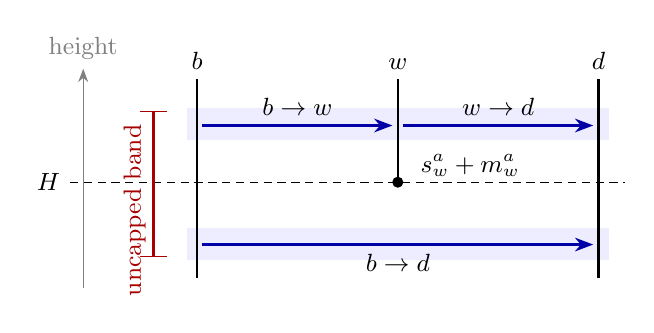
\begin{tikzpicture}[x=0.85cm,y=0.9cm,>=Stealth,
                    every node/.style={font=\small}]
 \fill[blue!7] (-0.15,2.1) rectangle (6.15,2.55);
 \fill[blue!7] (-0.15,0.4) rectangle (6.15,0.85);
 \draw[->,gray] (-1.7,0) -- (-1.7,3.1) node[above] {height};
 \draw[thick] (0,0.15) -- (0,2.95) node[above] {$b$};
 \draw[thick] (3,1.5) -- (3,2.95) node[above] {$w$};
 \draw[thick] (6,0.15) -- (6,2.95) node[above] {$d$};
 \draw[->,blue!65!black,thick] (0.08,2.3) -- (2.92,2.3);
 \draw[->,blue!65!black,thick] (3.08,2.3) -- (5.92,2.3);
 \draw[->,blue!65!black,thick] (0.08,0.62) -- (5.92,0.62);
 \node[above] at (1.5,2.3) {$b\to w$};
 \node[above] at (4.5,2.3) {$w\to d$};
 \node[below] at (3,0.62) {$b\to d$};
 \draw[densely dashed] (-1.9,1.5) -- (6.4,1.5);
 \node[left] at (-1.9,1.5) {$H$};
 \fill (3,1.5) circle (2pt);
 \node[anchor=west,fill=white,inner sep=2pt] at (3.25,1.73)
            {$s_w^a+m_w^a$};
 \draw[red!65!black,very thick] (-0.65,0.45) -- (-0.65,2.5);
 \draw[red!65!black] (-0.85,0.45) -- (-0.45,0.45);
 \draw[red!65!black] (-0.85,2.5) -- (-0.45,2.5);
 \node[anchor=east,rotate=90,red!65!black] at (-0.93,2.45)
            {uncapped band};
\end{tikzpicture}
\caption{A triple contact in height coordinates.  The shaded strips
indicate positive intervals of shared quantum-boundary heights;
they are not drawings of Euclidean seams.  The outer pair is linked
below $H$, while above $H$ each outer run is linked to the middle
run.  The middle run's exact discrete minimum caps the outer-pair
band.}
\label{inp:triple-figure}
\end{figure}

We use bands lying inside these shared height intervals with positive
margins at their effective endpoints, with two exceptions prescribed
by the record data.  At a natural lower record minimum the rational
band starts below the minimum and is clipped by the exact record
condition.  At an upper endpoint with the three-seam configuration,
the band is clipped by the exact selected minimum
\eqref{inp:exact-cap}.  These are the admissible band choices in
the proof of Lemma ``Finite-band reconstruction'' of
\cite{MetricMaps}.  All their tests use the local tagged frontiers,
relative increments, and quantum lengths just described.

\begin{samepage}
\begin{lemma}[Complete graph pieces in a buffer]\label{inp:complete-core}
Fix $K\Subset U$ in a coordinate chart.  Almost surely, there is a
finite prescription, selectable from the local cells in $U$ and their
frontier data, with the following property.  In a neighborhood of $K$,
its instruction graph agrees with the actual discrete graph, including
vertex equalities and all edge incidences, for all sufficiently large
resolutions in the coupling.  The same prescription can retain both
the primal and the dual graph.  One can require any fixed smaller
collar of this neighborhood before restricting the tests to it.

The prescriptions can be taken from the countable instruction scheme
above and chosen measurably using the fields and spatial cut marks
in $U$, with an arbitrarily small open buffer.  The assertion also
holds in the interior of a fixed interval cell, using only its
internal increment string.
\end{lemma}
\end{samepage}

\begin{proof}
We use the exact-incidence part of the proof of Lemma ``Finite-band
reconstruction'' in \cite{MetricMaps}.  We give the argument because
exactness, rather than an approximation of path costs, is essential
for energy tests.

Choose $r>0$ so that the closed $3r$-neighborhood of $K$ lies in $U$.
Properness bounds all its visit times in a finite window.  Refine the
Poisson cuts until every cell meeting this neighborhood has diameter
less than $r$.  Select all cells meeting the closed $2r$-neighborhood
of $K$ and merge consecutive selected cells into maximal runs.  These
runs are disjoint intervals; all visits sufficiently near $K$ lie in
them.  Their endpoints stay away from $K$, since otherwise the
neighboring cell would also have been selected.  Local traversal
data identify the selection: first inspect a slightly larger buffer
and require the portions around every visit to the smaller compact
to be flanked by marks while they remain in that buffer.  Properness,
continuity, and refinement make this condition hold eventually.
No global index for the retained runs is part of this inspection.

Consider one coordinate and two selected runs $b<d$ in chronological
order.  An outgoing point of $b$ and an incoming point of $d$ at
height $H$ are linked exactly when
\begin{equation}\label{inp:gap-test}
 H\le\min_{\text{between the two runs}} Z^a.
\end{equation}
The same assertion holds discretely, with the full-strip convention
for a matched step.  Split the intervening interval into selected
runs and omitted gaps.  If a limiting link projects near $K$, any
intervening time at its height represents that same continuum point.
It must therefore belong to a selected cell.  Thus every omitted-gap
minimum is strictly above the height of that link.  The relevant
endpoint pairs form a compact set, and there are only finitely many
gaps.  Their positive slack is consequently uniform: a sequence of
slacks tending to zero would limit to a contact in an omitted gap,
contrary to the selection.

An obstruction without slack can only be a minimum of a selected run.
At a triple contact, the three directed seams in
Figure~\ref{inp:triple-figure} identify the middle run and recover
its offset through \eqref{inp:seam-offset}.  Formula
\eqref{inp:exact-cap}, evaluated on the discrete string, supplies
the cap in \eqref{inp:bands}.  At a natural
lower seam endpoint, choose the lower rational band endpoint below
the record minimum; the exact incoming or outgoing record condition
then clips the band at that minimum.  This retains links at the
minimum as well as links at nearby lattice heights.

For every pair of runs, cover the compact set of relevant link heights
by finitely many such bands.  Choose each band to be admissible over
its entire effective height interval: that interval lies in a genuine
shared seam, its omitted-gap comparisons have positive slack, and
every allowed non-strict cap is the exact selected minimum just
described.  The natural record conditions provide the exact clipping
at lower seam endpoints.  Include the positive seam intervals
needed to read the relative heights, and retain a spanning forest
of these comparisons in each coordinate.  All needed offsets are
sums along that forest.  Seam directions specify the order of
linked runs and distinguish each middle cap; the instructions
do not need an order between unrelated runs.  Each band retains every discrete link
satisfying its rule.  Uniform contour convergence, the positive
omitted-gap slack, and the exact selected minima show two things:
every actual link near $K$ belongs to one of these bands eventually,
and every permitted link in those effective bands is an actual link
eventually.  In particular the latter assertion applies to any
permitted link with one endpoint over a smaller core collar: its
two limiting endpoints lie on the same shared-seam point and hence
remain inside the captured collar.  The
assertions hold simultaneously for all links, regardless of their
number.

Vertex equality is the same first-coordinate minimum test, so it is
captured as well.  Start a chain of enabled identifications at a
core representative.  Its first link is an actual identification
by the preceding band validity.  All visits to that actual vertex
have uniformly close projections, independently of the instruction
graph, and lie in the captured collar.  Inductively the next enabled
link is therefore actual as well and remains at that vertex.
Thus a peripheral chain cannot introduce an additional equality
at the core.  Horizontal tree traversals with the same identified
endpoint pair give one tree edge; no two distinct tree edges have
that pair.  Added edges are instead identified by their matched
step-occurrence pair, preserving distinct parallel edges.  Hence the
result is equality of graphs with incidences, not merely equality
of their path relations.  Applying the argument to the other
coordinate gives the dual conclusion.

All seam, cap, and positive-margin conditions are measurable in the
oriented local cells and frontier lengths.  Rational bands, integer
lower bounds on positive margins, and finite forest choices give a
countable selection rule.  Taking a further collar before the final
restriction gives the stated neighborhood of $K$.  Inside a fixed
interval cell, every visit to a compact subset of its interior lies
in that interval with a time margin; the same argument then uses
only its internal string.
\end{proof}

An arbitrary union of overlapping formal window copies need not be
an injective copy of a map subgraph.  The lemma asserts the existence
of \emph{complete} prescriptions, obtained from disjoint maximal
runs or from a freshly computed merged graph.  All comparisons to
the actual map below use these complete prescriptions.

\begin{lemma}[Spatial and value selectors]\label{inp:sandwich}
In the setting of Lemma~\ref{inp:complete-core}, suppose
$K\subset O$ with $K$ compact, $O$ open, and
$\overline O\Subset U$.  There is an interval selector on a complete
prescription which, eventually, includes every vertex projected into
$K$ and includes only vertices projected into $O$.  Several such
choices may be made together, for confinement and for each port set.

Let $u$ be continuous on a neighborhood of $\overline O$.  For any
two uniform value tolerances $0<\delta_-<\delta_+$, finite rational
interval constraints on selected visit labels can be placed between
the constraints $|v-u\circ\pi_m|\le\delta_-$ on a slightly larger
compact set and $|v-u\circ\pi_m|\le\delta_+$ on a smaller one.
All these comparisons hold simultaneously for every continuous
target through the same retained test library.
\end{lemma}

\begin{proof}
On the finitely many selected windows, the limiting parameterizations
are continuous.  Cover the inverse image of $K$ by finitely many
relative-time intervals with closures projecting inside $O$.
Their endpoints may be chosen from the prescribed dense countable
relative-time library.  Uniform projection accuracy and the complete
collar of Lemma~\ref{inp:complete-core} give the desired inclusions.
Select a vertex when any of its visits is in this union.  The same
argument applies to each port, while vanishing edge mesh allows an
induced-edge rule within the complete prescription.

For value constraints, refine the intervals until the oscillation of
$u\circ\eta$ on each is less than a fixed fraction of
$\delta_+-\delta_-$.  Choose a rational value interval between the
two allowed tolerances.  Impose it at every selected visit in that
interval, retaining all simultaneous constraints when a vertex has
several visits.  The strict tolerance gap and uniform projection
error give the two implications.  The construction chooses among
an already countable collection of tests; it does not add a new
exceptional null set for each target $u$.  Compact exhaustion and
rational positive tolerances therefore yield common measurable
versions for all continuous targets.
\end{proof}

The selector lemma compares variational values with strict margins.
It does not assert convergence for a prescribed sharp boundary.
For a crossing event, for example, choose smaller port and confinement
constraints and then relaxed constraints, both strictly inside the
desired geometry.  An intermediate selector produces actual paths
in the relaxed test, and any path family having the smaller clearance
can be included by a sufficiently relaxed selector.  Thus existence
of a strictly fitting test with finite limiting extremal length is
independent of the particular complete prescription.  Exhausted
energy values have the same property.  These conventions also make
readouts with a varying spatial center jointly measurable: all
membership and value comparisons use finite selectors with a strict
gap, followed by countable exhaustion.

\subsection{The conditional law of enlarged outputs}

We now identify the conditional law of the finite numerical arrays.
The proof is the finite-experiment argument of \cite{MetricMaps},
with the output vector enlarged before taking a subsequence.
The enlargement is harmless for a specific reason: every change
of density in that argument is a function of the inputs alone.

\begin{lemma}[Conditional transfer for numerical outputs]
\label{inp:kernel-transfer}
Consider finitely many packages as in Definition~\ref{inp:packages}.
Different packages use disjoint master blocks and disjoint offset
forests.  Sample their Poissonized strings independently; give their
durations, cuts, and offset vectors smooth positive densities, with
offsets discretized on the height lattice.  Retain any finite or
countable vector of compactified numerical tests of their instruction
graphs, including tests on both graphs.

Along a common subsequence the reference laws have disintegrations
\[
 \nu_r(\dd x_r)K_r(x_r,\dd y_r),
\]
where $x_r$ denotes the durations, cuts, increment strings, and
forest offsets, and $y_r$ denotes the numerical outputs.
Insert these blocks in the actual bilateral walk with positive
omitted gaps.  Conditional on the entire limiting contour and its
cuts, their output law is
\begin{equation}\label{inp:conditional-product}
             \bigotimes_r K_r(x_r,\dd y_r).
\end{equation}
The kernels are invariant under changes of positive reference
densities and under relabeling blocks or changing the forest basis.
They are compatible with jointly retained refinements and merged
tests.  These identities hold after selection from the countable
instruction library using the limiting contour and cuts.
\end{lemma}

\begin{proof}
This is the argument of Lemma ``Finite reference experiment and conditional
transfer'' in \cite{MetricMaps}.  We include its measure calculation
to specify its application to potentially discontinuous variational
outputs.

Write $\epsilon_m=m^{-1/2}$.  For one coordinate, order all selected
blocks chronologically as $1,\ldots,k$.  Let $s_i$ be their starts,
$e_i$ their net increments, and $g_i>0$ the intervening durations.
Complete the union of the package forests to a tree $T$ on these
blocks.  Give its extra offsets independent positive densities.
If the density on an edge $e$ is $\rho_e$, use lattice mass
\[
 r_{m,e}(a)=\int_{a-\epsilon_m/2}^{a+\epsilon_m/2}
                      \rho_e(u)\,\dd u,
 \qquad a\in\epsilon_m\mathbb Z.
\]
Let $p_t(j)$ be the transition mass of one coordinate of the
unscaled rate-one axial Poisson walk, so its variance rate is
$\sigma^2=1/2$.  The exact density of the actual relative starts
with respect to these reference offsets is
\begin{equation}\label{inp:density}
 W_m^a=
 \frac{\displaystyle\prod_{i=1}^{k-1}
       p_{mg_i}\bigl(\epsilon_m^{-1}(s_{i+1}-s_i-e_i)\bigr)}
      {\displaystyle\prod_{e\in T}r_{m,e}(a_e)}.
\end{equation}
Indeed, tree differences and consecutive differences are related
by an integer linear map with integer inverse, obtained by summing
along paths in $T$.  Its determinant is $\pm1$, so there is no
lattice multiplicity.  Multiply \eqref{inp:density} for the two
coordinates and include the density ratio for the durations and
cuts to obtain $W_m$.

On compact input sets with all gaps bounded below by a positive
constant, the local central limit theorem gives
\[
 \epsilon_m^{-1}p_{mt}(j)
 \longrightarrow
 (2\pi\sigma^2t)^{-1/2}
       \exp\{-x^2/(2\sigma^2t)\},
 \qquad x=\epsilon_m j,\quad \sigma^2=\tfrac12,
\]
uniformly in bounded $x$ and in such $t$.  The numerator and
denominator of \eqref{inp:density} have the same number of lattice
factors.  They cancel, leaving uniform convergence $W_m\to W$ to
a continuous finite function on these compact sets.

Conditional on the selected inputs, the omitted strings are
independent bridges and are independent of the numerical outputs.
Their rescaled laws converge uniformly on these input sets to
Brownian bridge laws.  For completeness, their finite-dimensional
densities are ratios of transition masses, so the preceding local
limit theorem applies.  On the first half of a bridge the density
relative to the free walk is bounded by
\[
 \frac{\sup_j p_{m(t-u)}(j)}{p_{mt}(j_0)}\le C,
 \qquad u\le t/2,
\]
when $t$ and $\epsilon_mj_0$ range in the chosen compact sets.
The numerator is at most $C\epsilon_m$ and the denominator at
least $c\epsilon_m$.  Free-walk tightness and the reversed argument
on the other half prove uniform bridge tightness.  The same applies
to a finite list of gaps and to exterior contour portions on a
bounded window.

The full independent reference experiments converge jointly to the
product of their limits, because their output spaces are compact
and their input marginals converge.  Let $a$ denote the completion
offsets and $z$ the omitted bridges.  Integrating bounded continuous
bridge tests first, the preceding uniform convergence gives the
limiting actual law
\begin{equation}\label{inp:weighted-law}
 W(x,a)\,\nu(\dd x,\dd a)\,
       \mathcal B(x,a;\dd z)\prod_rK_r(x_r,\dd y_r).
\end{equation}
The weight and the bridge law depend only on contour inputs.
The complete contour and cuts recover $(x,a,z)$, so disintegration
of \eqref{inp:weighted-law} gives \eqref{inp:conditional-product}.

To remove the compact restrictions, first keep all finitely many
limiting gaps positive, then bound endpoints and offsets, and
finally restrict the block paths to compact sets.  Under the actual
law the excluded probability tends to zero by finite-window contour
tightness.  If $P_m$ is the actual law and $Q_m$ the reference law,
the exact identity
\[
             \E_{Q_m}[W_m\1_{A^c}]=P_m(A^c)
\]
controls the omitted density mass.  No global bound on $W_m$ is
required.  Exhaustion, followed by a monotone-class argument, gives
the assertion for bounded measurable tests and for the entire
bilateral contour.

A change of reference density adds another input-only density
ratio, continuous in the limit on compact sets, and thus leaves
$K_r$ unchanged.  Forest bases are related by unimodular integer
maps.  The pushed-forward lattice cells and the directly discretized
cells have the same volume and vanishing diameter.  Their mass
ratios converge to one on compact sets; tightness makes the two
lattice laws converge in total variation.  This comparison remains
valid after applying a discontinuous graph-output map.  Absolute
time labels and the order of unrelated blocks occur only in
$W_m$, and disappear from the conditional output law.

For merged tests one must also check the old output.  Begin with
the old independent blocks, their offsets, and their old numerical
outputs.  Insert the formerly omitted positive-duration gaps by
the exact density and bridge construction.  The resulting string
has the new master-block law.  Recompute the old graph from its
unchanged active windows and bands, and compute the new union graph
as a separate output on that same string.  Formula
\eqref{inp:weighted-law}, applied before conditioning on the new
master string, proves the old conditional marginal.  It never
evaluates a previously chosen kernel on a forced-offset diagonal.
Windows with a common endpoint were already within one maximal
run, so no positive-density argument is applied to a zero-length
gap.  Jointly retaining finite vectors proves consistency for all
refinements and unions, and then for the countable library.

Every step used only compactness of the output coordinates and
their measurability from their own package.  Thus it applies to
the energy and extremal-length tests, with any deterministic
normalization.  It does not require continuity of those outputs
or preservation of conditional independence under arbitrary weak
limits.  Finally, after conditioning the identities hold for all
countably retained templates on one event; contour- and
cut-measurable selection from them is therefore permitted.
\end{proof}

\subsection{Spatial locality and changes of quantum units}

The preceding kernels are indexed by contour blocks.  To use them
in disjoint spatial regions, their inputs must be readable from
the fields in those regions.  This is where oriented cells and
relative frontier heights enter.

\begin{proposition}[Local numerical-array kernels]\label{inp:local-kernels}
On each open coordinate domain, take the limits of the numerical
tests on complete buffered prescriptions, with relative labels
localized to their cells.  Conditional on $(h,\widehat h)$, the
resulting local arrays admit kernels depending only on the fields
in an arbitrarily small open enlargement of the testing region.
Arrays using disjoint such enlargements are conditionally
independent given the complete fields.

One may retain the local Poisson marks.  Their conditional laws are
the corresponding Poisson processes with intensity proportional
to $\mu_h$, and their restrictions to disjoint domains are
independent.  The kernels are consistent under restriction,
common refinements, and compact exhaustion.
\end{proposition}

\begin{proof}
Proposition ``Background locality'' in \cite{MetricMaps}
states that $\widehat h$ in a buffer determines the oriented curve
segments through the testing region.  The restriction of $h$
gives their area parameterizations and their directed frontier
lengths.  These data determine the locally retained marked cells.
For a segment from time $s$ to time $t$, its coordinate increment
is the outgoing frontier length minus the incoming frontier
length of that coordinate, with tagged multiplicities retained:
\begin{equation}\label{inp:frontier-increments}
 Z^q_t-Z^q_s
   =\nu_h(\partial_q^{\mathrm{out}}\eta([s,t]))
      -\nu_h(\partial_q^{\mathrm{in}}\eta([s,t])),
 \qquad q\in\{L,R\}.
\end{equation}
Formula \eqref{inp:frontier-increments} reads
the increments without an absolute contour height.  Positive
shared seams read the forest offsets, and the three-seam
configuration in Lemma~\ref{inp:complete-core} reads the offsets
needed at a minimum cap.  Durations and relative cuts are local
area data.  Thus all four types of input in
Lemma~\ref{inp:kernel-transfer} are local.

For finitely many prescriptions in disjoint spatial domains,
merge within each domain.  Different domains use disjoint cells;
two runs from different domains cannot share a cut, since its
image would belong to both compactly contained cells.  Their
intervening chronological gaps are therefore positive even if
the runs interleave in time.  Lemma~\ref{inp:kernel-transfer}
gives their product law conditional on the contour and cuts.
Its invariance under labels and forest bases lets us enumerate
the cells locally without retaining a global cut index.

Adjoin the continuum background by the conditional sampling
convention above.  The product formula remains valid upon
conditioning additionally on the fields.  Its factors are now
measurable functions of the local fields and spatial marks,
by the preceding input reconstruction.  Conditional expectation
therefore gives the same product formula given the complete
fields and spatial marks.  This is exactly the argument of
Proposition ``Spatial product kernels'' in \cite{MetricMaps}, applied to the
enlarged output vector of Lemma~\ref{inp:kernel-transfer}.

The time cuts are independent of the continuum background.
Area parameterization and the Poisson
mapping theorem give their spatial conditional intensity
$\rho\mu_h$ for a layer of time intensity $\rho$.
Write $\Pi_i$ for the marks in the $i$th domain and
$K_i^{\mathrm{marks}}(h,\widehat h,\Pi_i;\cdot)$ for the
conditional output kernel already obtained.  Given the fields,
the marks have independent Poisson laws, and hence the output
law after removing them is
\[
 \bigotimes_i\int K_i^{\mathrm{marks}}
       (h,\widehat h,\pi_i;\cdot)\,
             \operatorname{Pois}_{\rho\mu_h|_{U_i}}(\dd\pi_i).
\]
This proves the fields-only assertion.  It uses no independence
between the marks and the numerical arrays, whose tests may
depend on those marks.  Alternatively, retain each $\Pi_i$
together with its array as the local output.
Finite joint consistency and the countable prescription library
then give the kernel on all tests.  Lemmas
\ref{inp:complete-core} and~\ref{inp:sandwich} identify its
buffered exhaustion with the corresponding observations from
the actual graph.  No additional conditioning on exterior
numerical outputs is used.
\end{proof}

\begin{proposition}[Coordinate and unit transport]\label{inp:transport}
The kernels in Proposition~\ref{inp:local-kernels} can be retained
jointly with the following transformations.
\begin{enumerate}
\item For a fixed conformal coordinate map $\phi$, pull back the
fields by
\[
 g\longmapsto g\circ\phi+Q\log|\phi'|,
 \qquad
 \widehat g\longmapsto\widehat g\circ\phi-\chi\arg\phi'.
\]
The numerical-array law is transported by the corresponding
spatial relabeling of its tests.
\item Fix $v=2^k$, $k\in\mathbb Z$, and put
$c_v=\gamma^{-1}\log v$.  Expressing the surface in the field
$g-c_v$ replaces area time by time divided by $v$ and replaces
rate $m$ by rate $mv$.  Electrical energies and extremal lengths
are unchanged by this relabeling.  If a numerical output is
divided by $b_m$, retain this same factor $b_m$ in the $mv$
experiment of the joint extraction.
\item Write $K_{(1)}$ for the original local law, including the
mark kernel, and $K_{(v)}$ for the law of the corresponding
transformed rate experiment.  Then
\begin{equation}\label{inp:unit-kernel}
 K_{(v)}(g,\widehat g)
     =\operatorname{Relabel}_v K_{(1)}(g+c_v,\widehat g).
\end{equation}
All fixed dyadic indices, their transformed templates, and the
required Poisson layers may be retained in one joint extraction.
\end{enumerate}
\end{proposition}

\begin{proof}
This is the finite-experiment identity underlying Proposition ``Intrinsic
transport and fixed quantum units'' in \cite{MetricMaps}.
A conformal change leaves quantum areas, frontier lengths,
directed seam roles, and their relative heights unchanged.
Hence it leaves the finite instruction graph unchanged and
only changes the projection of its labels.

Adding $c_v$ multiplies areas by $v$ and boundary lengths by
$\sqrt v$.  Thus the block inputs transform as
\begin{equation}\label{inp:block-units}
 \ell\longmapsto v\ell,
 \qquad z(t)\longmapsto\sqrt v\,z(t/v),
 \qquad o\longmapsto\sqrt v\,o.
\end{equation}
Cuts transform with time; band endpoints, their anchors, and
selected minima transform with height.  A rate-$m$ Poisson
string of duration $v\ell$ is, after this time change, a
rate-$mv$ string of duration $\ell$.  The height lattices agree
because $\sqrt v\,(mv)^{-1/2}=m^{-1/2}$.  Matching strips and
minimum comparisons are exactly the same integer tests.
Therefore the numerical costs on the resulting graph are
identical.  Smooth sampling densities may change, but
Lemma~\ref{inp:kernel-transfer} leaves the conditional kernels
unchanged.

The cuts must be transformed too.  At field $g+c_v$, the layer
corresponding to a fixed layer at field $g$ has time intensity
divided by $v$.  Its spatial intensity is then unchanged.
Choose a countable family of layers closed under these changes,
with independent layers and nested refinements as required.
Their joint input and output identities give
\eqref{inp:unit-kernel}.  A fixed field translation is locally
equivalent to the Gaussian reference law, as specified below;
this makes the identity valid under that fixed reference
marginal as well.  No estimate uniform in unbounded $v$ is
asserted or needed.
\end{proof}

For exhaustion of the plane we retain the joint cone normalization,
not only the deterministic-coordinate kernel identity.  In the
circle-average embedding define
\begin{equation}\label{inp:joint-zoom}
\begin{split}
 r_v&=\sup\{r>0:h_r(0)+Q\log r=c_v\},\\
 h^{(v)}&=h(r_v\,\cdot)+Q\log r_v-c_v,
 \qquad \widehat h^{(v)}=\widehat h(r_v\,\cdot),\\
 \eta^{(v)}(t)&=r_v^{-1}\eta(vt),
 \qquad Z^{(v)}(t)=v^{-1/2}Z(vt).
\end{split}
\end{equation}
The complete marginal has the original cone peanosphere law, by
the joint zoom in \cite{MetricMaps} and
\cite[Proposition~4.13(i)]{DMS}.  The positive dilation preserves
the independent stationary-phase imaginary-field law.  These
transformations are applied to the contour, raw arrays, and full
background together, before disintegration.  Thus field-dependent
reembedding does not require substituting a random map into
separately chosen versions of deterministic-coordinate kernels.
Moreover $r_{2^k}\to\infty$ as $k\to\infty$: the level $c_{2^k}$
diverges, whereas $h_r(0)+Q\log r$ is bounded above on compact
sets of radii and tends to $-\infty$ as $r\downarrow0$.
Ordinary patches inside these normalized disks therefore exhaust
the plane away from the cone point.

\begin{lemma}[Ordinary Gaussian reference patches]\label{inp:gaussian}
On a buffered patch compactly inside the cone's normalization
disk and away from its marked point, the actual real and
imaginary fields are locally equivalent to Gaussian reference
restrictions.  The real-field pinning circle can be fixed outside
all testing buffers.  This comparison preserves the actual
additive constant and can be made after any fixed affine change
of coordinates.

Adjoining any of the local kernels above preserves the same
field-only Radon--Nikodym derivative.  Consequently one fixed
density truncation transfers high-probability events uniformly
over all kernels attached to that reference marginal.  Fixed
additive real-field shifts and the fixed coordinate transforms
used in Proposition~\ref{inp:transport} preserve the corresponding
local null sets.
\end{lemma}

\begin{proof}
This is Lemma ``Ordinary cone patches and exterior Gaussian pins''
in \cite{MetricMaps}.  Inside the unit disk the circle-average
cone field has the law of the circle-average-zero whole-plane
GFF minus $\gamma\log|z|$.  On the patch, this deterministic
term has a smooth extension supported away from the marked
point and the pinning circle.  The Cameron--Martin theorem
and Gaussian domain comparison give local equivalence, with
the actual constant retained.  The same argument applies to
a fixed additive shift on the patch.  The imaginary field is
independent and is interpreted modulo its angular period;
its local restrictions have the corresponding Gaussian
equivalence and stationary-phase coordinate invariance.

If $Z=\dd\nu/\dd\mu$ is a field density and $K_i$ any of the
conditional kernels, then for every event $A$ and every $R>0$,
\begin{equation}\label{inp:density-truncation}
 (\nu\otimes K_i)(A)
 \le R(\mu\otimes K_i)(A)
      +\E_\mu[Z\1_{\{Z>R\}}].
\end{equation}
The last term does not depend on $i$.  This proves the uniform
probability comparison; local equivalence gives both directions
for probability-one events.  A test domain containing the full
pinning circle is excluded by the stated buffer condition.
\end{proof}

\begin{lemma}[Primal--dual reflection]\label{inp:reflection}
The joint local-array laws are invariant under exchanging the
primal and dual graphs and reflecting their coordinate tests.
They are also covariant under fixed rigid motions, with the
natural transformations of the two fields.
\end{lemma}

\begin{proof}
The discrete assertion follows by exchanging the two independent
coordinate strings and their forests.  In the continuum,
spatial reflection combined with negation of the reflected
imaginary field exchanges the two angle trees and the two
sides of the curve.  The space-filling ordering is preserved:
it can be read either from the $+\pi/2$ tree with right merges
or from the $-\pi/2$ tree with left merges, as in
\cite[Section~1.2.3, Figure~1.16]{IG4}.  Both descriptions are
exchanged by this operation, so no reversal of area time is
involved.  The cone field and the independent stationary-phase
imaginary field have the required reflected law.  Boundary
lengths exchange $L$ and $R$, and conditional sampling of the
background therefore gives the same operation on the joint
raw-array limit.  The intrinsic kernels and the selector
construction then transport the spatial tests.  Fixed rotations
and translations follow from coordinate covariance and local
field equivalence on buffered ordinary patches.  A countable
group of such transformations can be retained simultaneously.
\end{proof}

\begin{proposition}[Local-array interface]\label{inp:array-interface}
From every sequence of resolutions tending to infinity one can
extract, jointly with the continuum peanosphere background,
all compactified numerical tests described above, on both
graphs and at every fixed dyadic area offset.  Prescribed
deterministic normalizing factors may be retained even when
they tend to zero.  In this extraction:
\begin{enumerate}
\item complete buffered graph pieces and the selector sandwich
of Lemmas~\ref{inp:complete-core} and~\ref{inp:sandwich} identify
local tests with actual graph observations;
\item Proposition~\ref{inp:local-kernels} supplies buffer-local
conditional kernels and product laws in disjoint domains;
\item Proposition~\ref{inp:transport} and
Lemmas~\ref{inp:gaussian}--\ref{inp:reflection} supply their
coordinate, unit, Gaussian-reference, and primal--dual
comparisons;
\item these properties persist under further joint extraction
and under countable exhaustion with strict margins.
\end{enumerate}
\end{proposition}

\begin{proof}
All numerical coordinates belong to compact spaces, and the
input contours are tight on bounded windows.  Include the
countable transformed instruction lists and mark layers before
the diagonal extraction.  The preceding results apply to
every finite collection.  Their exact density and bridge
calculation passes to any further limit by compact truncation;
the continuum background passes by the $L^1$ conditional
sampling argument.  Countable intersection and the selector
exhaustions give the stated simultaneous version.
\end{proof}

The interface provides laws and exact local observability.
The bounds which prevent degeneration of the electrical tests,
and the identification of their variational limits, are proved
next.

\section{Nondegeneration of the electrical networks}
\label{sec:nondegeneration}

We first prove that a fixed conformal annulus admits cutoffs of bounded
electrical energy on both sewn graphs.  The bound will depend on the
annulus aspect and the coordinate patch, but not on its radius or the
discrete resolution.  This is the coercivity input for the variational
argument in the next section.  Throughout this section we work with
the bilateral sewing, at rates $m\to\infty$, and use the coupled
extractions and projections $\pi_m$ of
Proposition~\ref{inp:array-interface}.

The proof combines two uses of extremal length.  A lower bound supplies
densities that charge every crossing of an annulus.  If lower bounds
failed, a suitable quantile would instead supply probability measures
on crossing paths with very small squared traffic.  Annular densities
make their projected limits rectifiable.  Locality then forces a
transverse crossing witness on the other graph, contradicting the
small traffic.  The annular-density, rectifiable-flow, and local-germ
strategy is developed for flag extremal length in
\cite[Section ``The canonical conformal structure'']{ConformalMaps}.
We adapt it to edge energies on paired primal and dual graphs.

\subsection{Extremal length and local germs}

Let $\mathcal P$ be a nonempty family of paths in a finite graph, with
no path of length zero.  Edge occurrences are counted with
multiplicity.  Its edge extremal length is
\begin{equation}\label{nd:el-definition}
 \EL(\mathcal P)
 =\sup_{a:E\to[0,\infty)}
   \frac{\bigl(\inf_{P\in\mathcal P}\sum_{e\in P}a(e)\bigr)^2}
        {\sum_{e\in E}a(e)^2},
\end{equation}
where the zero density is omitted.  For a probability measure $\nu$
on paths, write
$j_\nu(e)=\int \#\{\text{occurrences of }e\text{ in }P\}\,\nu(\dd P)$
for its unsigned edge traffic.

\begin{lemma}[Densities and traffic]\label{nd:el-traffic}
For a finite family of simple paths,
\begin{equation}\label{nd:traffic-identity}
 \EL(\mathcal P)=\min_{\nu}\sum_e j_\nu(e)^2.
\end{equation}
If $\mathcal P$ consists of all paths between two disjoint wired sets
in a finite subgraph, then $\EL(\mathcal P)$ is the reciprocal of
the minimum energy $\en(u)$ subject to the values zero and one on
the two sets.  In particular, $\EL(\mathcal P)\ge b>0$ supplies a
density charging each path by one with squared norm at most $1/b$.
\end{lemma}

\begin{proof}
The traffic vectors form the convex hull of the path-incidence
vectors.  Let $j$ be its point nearest to the origin.  The supporting
inequality $\langle j,j_P\rangle\ge\|j\|_2^2$ for every path $P$
shows that the density $j$ gives a value at least $\|j\|_2^2$ in
\eqref{nd:el-definition}.  Conversely, averaging path length under
any $\nu$ and applying Cauchy--Schwarz gives
$\EL(\mathcal P)\le\|j_\nu\|_2^2$.  This proves
\eqref{nd:traffic-identity}.  In the wired-set case loops may be
removed from paths.  Absolute potential increments give a charging
density, while the distance from the first set in any charging
density, clipped at one, gives an admissible potential whose energy
is at most the squared density norm.  These two constructions prove
the reciprocal identity.
\end{proof}

We will also use a consequence of the local conditional kernels from
Section~\ref{sec:inputs}.  A \emph{point-germ readout} is a jointly
measurable random function $Y(z)$ whose value at $z$ can be read from
the fields and extracted arrays in every neighborhood of $z$.  The
readout may use countably many tests with strictly positive domain
margins.  In particular, an assertion that specified tests succeed
at every sufficiently small scale is a point-germ readout.

\begin{lemma}[Determinism of point germs]\label{nd:germs}
In an ordinary field chart, every bounded real point-germ readout
of the extracted local arrays is, almost surely, equal at
Lebesgue-almost every point to a deterministic measurable function
of the point.  The same conclusion holds for readouts with values
in a separable metric space, using a countable family of bounded
coordinates that separates its points.
\end{lemma}

\begin{proof}
Let $\mathcal H$ denote the pair of fields.  By
Proposition~\ref{inp:local-kernels},
$\E[Y(z)\mid\mathcal H]$ is measurable with respect to the field
restrictions to every neighborhood of $z$.  This field germ is
trivial.  Indeed, for a zero-boundary Gaussian free field, the
intersection of the Gaussian subspaces generated by restrictions
to shrinking disks is orthogonal to the Gaussian variables
associated with Dirichlet functions vanishing near $z$.  Such
functions are dense in the Dirichlet space: logarithmic cutoffs
express the zero capacity of a point.  The intersection is thus
zero, and the Gaussian chaos decomposition gives triviality of
the corresponding sigma-field.  Apply this to both independent
fields.  Local equivalence in Lemma~\ref{inp:gaussian}
transfers the conclusion to the ordinary chart, including the
imaginary field modulo its period.  Consequently
$\E[Y(z)\mid\mathcal H]=y(z)$ for a deterministic $y$.

For distinct $z,w$, disjoint sufficiently small neighborhoods and
the product-kernel assertion give conditional independence of
$Y(z)$ and $Y(w)$ given $\mathcal H$.  Hence, for every rational
disk $D$ compactly in the chart,
\[
 \E\left[\left(\int_D(Y(z)-y(z))\,\dd z\right)^2\right]=0.
\]
The diagonal in $D\times D$ has Lebesgue measure zero.  Countably
many disks and differentiation of integrals prove the assertion.
Applying the argument to bounded separating coordinates proves
the final statement.
\end{proof}

\begin{remark}[Coordinate and dual symmetries]\label{nd:germ-symmetries}
For a readout defined intrinsically from local tests, its deterministic
values respect the coordinate transports of
Proposition~\ref{inp:transport}.  More explicitly, let $\mathcal A$
be the extracted local array and let $T\mathcal A$ denote its
relabeling by a fixed translation or rotation $T$.  A covariant
readout satisfies
\[
             Y_{T\mathcal A}(Tz)=T\cdot Y_{\mathcal A}(z),
\]
where $T\cdot$ is the natural action on its values or direction
labels.  The transport proposition identifies the law of
$T\mathcal A$ with the same extracted kernel attached to the
transformed fields.  Local equivalence of these field laws and
Lemma~\ref{nd:germs} therefore give
$y(Tz)=T\cdot y(z)$ almost everywhere.  This uses a relabeling in
the joint extraction, rather than a newly chosen subsequential
kernel.  For translation-covariant scalar readouts it implies
constancy: first use rational translations, then continuity of
translations in local $L^1$.  Rotations act on direction or matrix
readouts in the stated natural way, and a countable dense rotation
group suffices.  Finally, Lemma~\ref{inp:reflection} exchanges the
two graphs and reflects the tests.  These observations apply on
overlapping ordinary charts and identify their deterministic values.
The definition through strict margins is important here: a transported
test is still an admissible test after an arbitrarily small reduction
of its clearance, by Lemma~\ref{inp:sandwich}.
\end{remark}

\subsection{Annular barriers at absolute quantum scales}

Choose once and for all an ordinary cone patch, strictly inside
the normalization disk and away from the cone point.  After a
fixed affine coordinate change, it contains the annulus
$\{1/16<|z|<4\}$ and the buffers needed below.
For each graph take paths between the vertex sets selected by visits
in the bands
\[
 A_1=\{.9<|z|<1.1\},\qquad
 A_2=\{1.9<|z|<2.1\},
\]
confined to the actual subgraph selected in
$A_0=\{.7<|z|<2.3\}$.  Denote the extremal lengths of these primal
and dual path families by $Z_m^{\mathrm p}$ and $Z_m^{\mathrm d}$.
Here selection uses the continuum visit labels
in the coupling, with a fixed step-endpoint convention.  This defines
a comparison variable; it need not itself be a local instruction
test.  Properness makes the selected labels finite.  All their
incidences and adjoining star layers are protected in larger bounded
contour windows.  The projection and tube properties of
Proposition~\ref{inp:topology} therefore apply.  If the ports overlap
or there is no crossing, give the comparison the value one.  The
probability of these exceptions tends to zero.

Let $Z_m=\min\{Z_m^{\mathrm p},Z_m^{\mathrm d}\}$.  Fix
$\varepsilon>0$, to be chosen below, and choose deterministic
$q_m>0$ such that
\begin{equation}\label{nd:quantiles}
 \P[Z_m\le 2q_m]\ge\varepsilon/2,
 \qquad
 \P[Z_m\ge q_m/2]\ge1-2\varepsilon.
\end{equation}
We use rates in a countable set closed under dyadic multiplication
and division, for example the positive dyadic rationals.  The
quantiles can be chosen bounded below on every bounded rate interval
in $[1,\infty)$.  To see this, first bound the continuum preimage
window with high probability, then bound the Poisson step count
and the degrees of the finitely many encountered vertices.  Local
finiteness of the bilateral sewing makes these bounds uniform at
bounded rates.  A nonexceptional finite graph with at most $L$
edges has positive crossing extremal length at least $1/L$.

The comparison in \eqref{nd:quantiles} produces genuinely local
barrier events.  For example, select ports near radii $.96$ and
$2.04$, and confinement between $.94$ and $2.06$, with strictly
positive slack.  Every path from $\{|z|<.6\}$ to
$\{|z|>2.5\}$ contains such a crossing portion.  A complete local
prescription covering this intermediate shell exists by
Lemma~\ref{inp:complete-core}; Lemma~\ref{inp:sandwich} selects the
ports and confinement.  Its path family is a subfamily of the
comparison family, so its EL is no smaller.

The selection can depend on the limiting fields without changing
this probability comparison.  To see the quantifiers, let $j$
enumerate pairs of primal and dual prescription templates.  Let
$\mathsf A_j$ be the local event that both templates' seam, cap, and
positive-margin conditions cover the required shell and implement
the selector sandwich.
These conditions are read from the local fields and marks;
their proved consequence is eventual completeness on the actual
graph.  They do not test completeness by inspecting exterior
numerical arrays.  For any deterministic units $b_m>0$ retained
in the extraction, write $\xi_j$ for the minimum of the two
retained limits of $\EL/b_m$.  Thus success supplies barriers on
both graphs.  If a comparison event asserts
$Z_m/b_m\ge a>0$, retain its indicator in a further coupling.
On the event $E$ where the limiting indicator is one, choose
an applicable $j$ from the limiting local cell data, keeping it
fixed as $m\to\infty$.  Its eventual domination of the comparison
gives $\xi_j\ge a$.  Consequently
\[
 E\subseteq\bigcup_j\bigl(\mathsf A_j\cap\{\xi_j>a/4\}\bigr).
\]
The union on the right is a local event with at least the
limiting comparison probability.  Simultaneous convergence of
the countably retained tests justifies the random choice of
$j$; no deterministic bound on that index is required.  This
argument uses the comparison for its probability and the local
union for its conditional kernel, without conditioning that
kernel on $E$.

We recall precisely the annulus input that spreads these barriers
through a chart.  It is Lemma ``All-point absolute quantum-scale
annuli'' in \cite[Section ``Annuli at absolute quantum scales'']{MetricMaps}.
Write $v_i=2^{-i}$ for the backward quantum-area offsets.  By
Proposition~\ref{inp:transport}, graph costs are unchanged at these
offsets; any deterministic denominator $b_m$ is kept the same
across the offset experiments in one extraction.

\begin{lemma}[Aligned annular barriers]\label{nd:coverage}
Fix an ordinary chart and a compact subset of its interior.  Suppose
that, at every fixed backward index $i$, a local unit-annulus event
has probability at least $1-\varepsilon_*$ in the reference law and
supplies, on both graphs, a crossing density of charge one and
squared norm at most $C/b_m$.  Here $b_m>0$ is deterministic and
the events belong to the common extracted offset kernels.
For a sufficiently small reference threshold $\varepsilon_*>0$,
there are constants $0<a<B$, $c>0$ such that the following holds
almost surely for all sufficiently large integers $N$.
Every point in the compact set belongs to the central holes of at
least $cN$ pairwise disjoint buffered annuli whose local barrier
events hold.  Their radii belong to one fixed geometric sequence
in $[e^{-BN},e^{-aN}]$, their centers lie on deterministic meshes
of spacing comparable to their radii, and their assigned indices
belong to $\{N,\ldots,2N\}$.
For each fixed such finite configuration, its density conclusions
hold on the discrete graphs for all sufficiently large $m$.
\end{lemma}

\begin{proof}
Apply the cited lemma to the kernels of
Proposition~\ref{inp:local-kernels}, with the intrinsic transport
of Proposition~\ref{inp:transport}.  Its hypotheses are the local
product rule, the actual-field coordinate rule, and a common
fixed-index change of quantum unit; all are supplied by
Proposition~\ref{inp:array-interface}.  The real-field parameter
$Q=2/\gamma+\gamma/2$ is greater than two.  The cost-index factor
in the stated annulus lemma is undone in our numerical tests;
the proof of that lemma uses the factor only in the indexed
observation rule.  Thus it applies equally to the present
unchanged network costs.  Local Poisson marks are included in
the kernels with their corresponding intensities.

For completeness, the probability transfer needed here is a fixed
one.  Work first with the zero-boundary Gaussian reference patch
of that lemma.  Local equivalence, retaining the actual additive
constant of the real field, gives a single absolute-continuity
modulus from our chosen ordinary cone patch to this reference
patch.  Choose $\varepsilon$ in \eqref{nd:quantiles} sufficiently
small that a barrier event of probability $1-2\varepsilon$,
with a strict threshold as above, has reference probability at
least $1-\varepsilon_*$.  The annulus lemma gives an exponentially
small failure probability at scale $N$.  Borel--Cantelli gives
the eventual assertion.  A fixed local change of field law
transfers this probability-one assertion to any ordinary chart.
No likelihood bound uniform over those charts is needed.
Finally, success of an annulus is the existence of a retained
EL coordinate strictly above a fixed threshold.  No density or
path is retained as an additional output.  All centers, radii,
indices, and prescription templates belong to countable
libraries.  On their simultaneous convergence event, the
successful local prescription on each realized annulus gives
an eventual discrete EL lower bound.  Lemma~\ref{nd:el-traffic}
then constructs a density on that finite graph.  For fixed $N$
only finitely many annuli are used, so their thresholds in $m$
can be met simultaneously, even though the successful annuli
and prescriptions were selected from the fields and arrays.
Thus $N$ is fixed before $m$ is sent to infinity.
\end{proof}

The geometric content of these many annuli is an area bound for a
density that charges macroscopic displacement.  For a set $U\subset\C$
write $U^{+r}=\{z:\dist(z,U)<r\}$, and put $R_N=e^{-aN}$.

\begin{lemma}[Densities controlling displacement]\label{nd:densities}
Under the hypotheses of Lemma~\ref{nd:coverage}, let $U$ be a finite
union of open boxes compactly in a fixed ordinary chart.  For all
sufficiently large $N$, and then all sufficiently large $m$, there
is on either graph a nonnegative density $g_{m,N,U}$, supported
near $U$, such that
\begin{equation}\label{nd:density-area}
 b_m\sum_e g_{m,N,U}(e)^2
       \le C\vol(U^{+CR_N}).
\end{equation}
Every path subinterval whose projection is contained in $U$ pays
at least
\begin{equation}\label{nd:density-charge}
 c\diam(\pi_m(P))-CR_N-o_m(1).
\end{equation}
The constants depend only on the smaller chart and the fixed
annular geometry.  The error and the threshold in $m$ may depend
on $N$ and $U$.  Charges add over disjoint path subintervals.
\end{lemma}

\begin{proof}
On a successful shell of radius $r$, multiply its barrier density
by $r$.  Its charge is now $r$ and its squared norm is at most
$Cr^2/b_m$.  Sum these densities over the shells whose central
holes meet $U$, using one density for each geometric shell, and
divide by $N$.  At any fixed radius the buffered shells have
bounded overlap, because their centers lie on a mesh of comparable
spacing.  There are at most $CN$ radii.  Cauchy--Schwarz across
these radii gives \eqref{nd:density-area}; all the involved shells
lie within distance $CR_N$ of $U$.

For the charge estimate choose a coordinate in which the projected
path has oscillation comparable to its diameter.  Consider levels
between its extreme values, discarding $CR_N$ near either end.
At a visit to each remaining level, the point lies in at least
$cN$ central holes.  Since all these shells have radius at most
$R_N$, the path crosses each of them before reaching a suitable
extreme.  A shell of radius $r$ can account for at most $Cr$ of
the levels.  Integrating over levels therefore bounds the total
length in the summed densities from below by $cN$ times the
remaining coordinate oscillation.  Divide by $N$.  At fixed $N$
the vanishing projected mesh permits full-edge crossing portions;
the discarded endpoint pieces contribute $o_m(1)$.  Distributing
each edge's density uniformly along that edge permits fractional
first and last edges and makes additivity over disjoint intervals
explicit.
\end{proof}

\subsection{Small traffic would force transverse crossings}

We now prove the quantitative fact needed for unnormalized energies.
\begin{proposition}[Nondegeneration]\label{nd:nondegeneration}
For the quantiles in \eqref{nd:quantiles}, with $\varepsilon$ chosen
as in Lemma~\ref{nd:coverage},
\begin{equation}\label{nd:positive-quantile}
                    \liminf_{m\to\infty}q_m>0.
\end{equation}
The conclusion holds along all rates in the chosen countable set.
\end{proposition}

\begin{proof}
Suppose otherwise.  Choose approximate record lows $m\to\infty$
such that $b_m:=q_m\to0$ and
\[
 q_s\ge c b_m\qquad(1\le s\le m,\ s\text{ in the chosen rate set})
\]
for a fixed $c>0$.  The bounded-rate lower bounds ensure $m\to\infty$.
For each fixed $i$, the quantile at $m2^{-i}$ therefore gives the
high-probability barrier event in units $b_m$.  Extract jointly
with all these backward offsets.  Lemmas~\ref{nd:coverage} and
\ref{nd:densities} apply in the comparison region.

The first inequality of \eqref{nd:quantiles} and
Lemma~\ref{nd:el-traffic}, on the other hand, supply with positive
probability one graph's probability flow $\nu_m$ between the two
macroscopically separated ports, confined in a fixed compact set,
with
\begin{equation}\label{nd:small-traffic}
                      \sum_e j_{\nu_m}(e)^2\le Cb_m.
\end{equation}
Retain the event indicator, choose a graph on a positive-probability
subevent, and work pathwise in a further coupling.  We establish
two properties of the projected flows before using locality.

\emph{Compactness of the flows.}
For a path $P$, let $J_h(P)$ be the maximum number of disjoint
subintervals making a projected advance of at least $h$.  Choose
$N$ large enough that $CR_N<ch/2$ in
\eqref{nd:density-charge}, and then take $m$ large.  Use a fixed
larger box union $U$ containing the compact confinement.  By
\eqref{nd:density-area}, \eqref{nd:small-traffic}, and
Cauchy--Schwarz,
\begin{equation}\label{nd:crossing-count}
 \int J_h(P)\,\nu_m(\dd P)\le C/h.
\end{equation}
Thus the paths are tight after reparameterization.  One explicit
choice of parameters is useful.  At every dyadic $h=2^{-l}$ place
clock atoms at successive completed moves of distance $h$, each
with mass $2^{-l}/(1+J_h(P))$.  Add the original traversal time
of total mass one, invert this clock with pauses at its atoms,
and rescale its total duration to one.  On sets where every
$J_{2^{-l}}$ has a fixed bound, these parameterized paths are
equicontinuous: an oscillation of several times $2^{-l}$ must
cross a whole atom interval of a fixed positive duration.
The bounds \eqref{nd:crossing-count} and a countable union bound
make such sets have arbitrarily large flow probability.  The
finitely many initial resolutions omitted at an individual scale
can be included by enlarging its bound.  A subsequence therefore
converges to a probability law $\nu$ on continuous paths.  Their
endpoints remain separated.

\emph{An absolutely continuous measure of arclength.}
For at most $J$ disjoint path intervals compactly confined in an
open box union $U$, the same argument gives
\begin{equation}\label{nd:variation-bound}
 \int\sup\sum_{k=1}^{J}
       |\pi_m(P(t_k))-\pi_m(P(s_k))|\,\nu_m(\dd P)
 \le C\sqrt{\vol(U^{+CR_N})}+CJR_N+o_m(1).
\end{equation}
The supremum may be taken over rational intervals with closure
in the prescribed open condition.  It is lower semicontinuous
under uniform convergence.  Pass first to the path limit, next
let $N\to\infty$, and finally let $J\to\infty$.  These interval
sums exhaust variation on open sets.  With a larger $U$ containing
all paths, they first show that $\nu$-almost every path is
rectifiable with integrable length.  Its average arclength
measure $\Lambda$ consequently satisfies
\begin{equation}\label{nd:length-area}
 0<\Lambda(\C)<\infty,
 \qquad \Lambda(U)\le C\sqrt{\vol(U)}.
\end{equation}
The positivity follows from the separated endpoints.  Open box
covers now show $\Lambda\ll\vol$.

We next convert a tangent of a limiting path into a local event.
Choose a sufficiently fine finite grid $\mathcal W$ of unoriented
directions, closed under quarter-turn and reflection in a coordinate
axis.  For $z\in\C$, $w\in\mathcal W$, and $s>0$, consider the tube
\begin{equation}\label{nd:tube}
 T(z,w,s)=\{z+tw+lw^\perp: |t|<2s,\ |l|<s/16\}.
\end{equation}
A \emph{strict crossing test} in this tube has ports strictly
beyond the two lines $t=-s$ and $t=s$, and has confinement and
ports with positive clearance from the tube boundary.  It is
computed on a complete local prescription.  Accept all countably
many selectors with these properties, and require that the
prescription be readable within a fixed-factor enlargement of
the tube, with positive margins.  Lemma~\ref{inp:sandwich} makes
existence of such a test independent of the particular selector
library after arbitrarily small relaxation of the margins.

At $\Lambda$-almost every point there is a direction $w\in\mathcal W$
for which, at every sufficiently small dyadic scale $s$, one of
these tests on the graph supplying $\nu_m$ has finite limiting
$\EL/b_m$.  Indeed, arclength parameterization gives a unit tangent
at almost every parameter of almost every rectifiable path.  The
fine direction grid puts that tangent inside one of the tubes
with strict slack at all sufficiently small scales.  Almost
every path is in the support of $\nu$.  The existence of the
strict crossing subpath is an open path event, so it has positive
$\nu$-probability at each such fixed scale.  Restrict $\nu_m$ to
this event, take the crossing portions, and normalize.  Its traffic
still has squared norm $O(b_m)$, with a constant allowed to depend
on the scale and the event probability.  The complete-selector
sandwich gives the asserted finite limiting test value.  The
statement can be imposed simultaneously at the countably many
dyadic scales.

Let $I^{\mathrm p}_w(z)$, respectively $I^{\mathrm d}_w(z)$, be the
indicator of existence of these finite-$\EL/b_m$ tests at every
sufficiently small dyadic scale, on the primal or dual graph.
These are jointly measurable point-germ readouts: the tests and
their fixed-factor buffers eventually lie in every neighborhood
of $z$.  The preceding paragraph and \eqref{nd:length-area} give
a positive-area set of witnesses on our positive-probability
event.  Lemma~\ref{nd:germs} and
Remark~\ref{nd:germ-symmetries} therefore imply that one of these
indicators has deterministic value one almost everywhere in
ordinary charts.  Reflection exchanges the graphs; rotations
within the finite direction grid then give the other graph's
indicator in the perpendicular direction.  The null sets can
be discarded simultaneously, since only finitely many directions
and two graphs are involved.

Choose a point with both perpendicular indicators equal to one,
and then a sufficiently small common dyadic scale.  We obtain
primal and dual strict crossing families with
$\EL=O(b_m)$ in perpendicular tubes, as illustrated in
Figure~\ref{nd:transverse-figure}.  Every path of one family meets
every path of the other upstairs by the transverse-tube rule in
Proposition~\ref{inp:topology}.  Such an intersection uses an edge
and its dual.  Choose traffic minimizers $j_m,j_m^*$ by
Lemma~\ref{nd:el-traffic}.  Their unsigned pairing satisfies
\[
 1\le\sum_e j_m(e)j_m^*(e^*)
    \le\Bigl(\sum_e j_m(e)^2\Bigr)^{1/2}
       \Bigl(\sum_{e^*}j_m^*(e^*)^2\Bigr)^{1/2}
    =O(b_m),
\]
contradicting $b_m\to0$.  This proves
\eqref{nd:positive-quantile}.
\end{proof}

\begin{figure}[t]
\centering
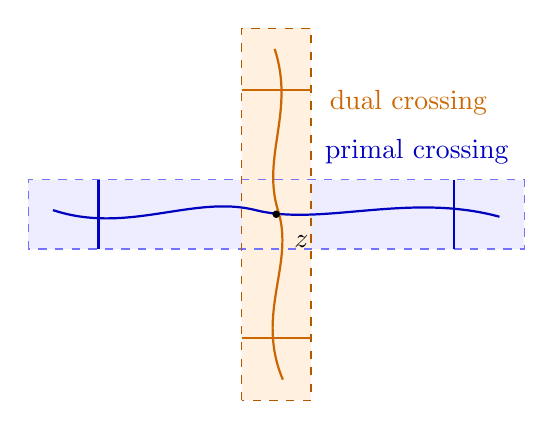
\begin{tikzpicture}[scale=1.05]
 \fill[blue!7] (-3,-.42) rectangle (3,.42);
 \fill[orange!12] (-.42,-2.25) rectangle (.42,2.25);
 \draw[blue!55,dashed] (-3,-.42) rectangle (3,.42);
 \draw[orange!70!black,dashed] (-.42,-2.25) rectangle (.42,2.25);
 \draw[blue!75!black,thick]
   (-2.7,.05) .. controls (-1.8,-.25) and (-1,.24) .. (-.25,.05)
   .. controls (.55,-.15) and (1.6,.27) .. (2.7,-.03);
 \draw[orange!80!black,thick]
   (.08,-2) .. controls (-.26,-1.2) and (.23,-.6) .. (.02,.05)
   .. controls (-.18,.7) and (.23,1.25) .. (-.02,2);
 \draw[blue!75!black,thick] (-2.15,-.42)--(-2.15,.42);
 \draw[blue!75!black,thick] (2.15,-.42)--(2.15,.42);
 \draw[orange!80!black,thick] (-.42,-1.5)--(.42,-1.5);
 \draw[orange!80!black,thick] (-.42,1.5)--(.42,1.5);
 \node[blue!75!black,anchor=south] at (1.7,.49) {primal crossing};
 \node[orange!80!black,anchor=west] at (.53,1.35) {dual crossing};
 \fill (0,0) circle (1.3pt);
 \node[anchor=north west] at (.1,-.14) {$z$};
\end{tikzpicture}
\caption{The two narrow tubes force transverse passages.  The drawing
shows only projected path ranges; it asserts neither injectivity of
the projection nor shape control of discrete edges.  The topological
input lifts this configuration to an intersection of a primal edge
with its paired dual edge.}
\label{nd:transverse-figure}
\end{figure}

\subsection{Uniformly bounded ring cutoffs}

We can now apply the annular construction in constant energy units,
rather than the hypothetical vanishing units used in the contradiction.

\begin{proposition}[Ring cutoffs]\label{nd:cutoffs}
Fix a compact subpatch of an ordinary chart and an aspect ratio
$\tau>1$.  Along a coupled further extraction from any rate sequence,
there is a constant $C$, depending only on the chart and $\tau$,
with the following property.  For every fixed disk
$\overline{B(z,\tau r)}$ contained with a margin in that subpatch,
both graphs eventually admit functions $\chi_m$ valued in $[0,1]$
such that
\[
 \chi_m=1\quad\text{on every lift of }\overline{B(z,r)},
 \qquad
 \chi_m=0\quad\text{on every lift outside }B(z,\tau r),
 \qquad
 \en(\chi_m)\le C
\]
on the primal graph, with $\enstar(\chi_m)\le C$ on the dual.
Their energy is supported in the indicated ring, up to vanishing
projected mesh.  The constant is independent of $z,r,m$; the
threshold in $m$ may depend on the fixed disk.  These assertions
hold simultaneously for the countable buffered disk tests, and
extend to arbitrary fixed disks by strict inner and outer margins.
\end{proposition}

\begin{proof}
Proposition~\ref{nd:nondegeneration} and the second quantile bound
in \eqref{nd:quantiles} give the barrier hypotheses with
deterministic units equal to one, at every fixed backward offset.
Choose an intermediate closed ring whose two radii lie strictly
between $r$ and $\tau r$, with all three resulting radial widths
comparable to $(\tau-1)r$.  Cover it by a finite union $U$ of open
boxes with closure strictly inside the target ring and area
$O_\tau(r^2)$.  Apply Lemma~\ref{nd:densities} to this $U$.
First choose $N$ so large that $R_N$ is small compared with the
intermediate width and both collars, and then take $m$ large.
The density is supported in the target ring.  Every full ring
crossing has a subcrossing through the intermediate ring,
confined to $U$, with advance comparable to $(\tau-1)r$.
The density therefore charges it by a fixed multiple of this
width.  After division by the width, the squared density norm
is bounded by $C(\tau)$ times the chart constant.
The clipped-distance construction of
Lemma~\ref{nd:el-traffic} gives the cutoff, with exact constants
on all inner and outer lifts.  One may carry out the construction
on a protected capped sphere and extend by constants beyond the
chart.  Only the ring density changes the function.

Countable buffered comparisons make all the fixed tests available
in one extraction.  A disk outside the chosen countable library
is handled by choosing a nearby library center, an inner library
disk containing $\overline{B(z,r)}$, and a concentric outer library
disk contained in $B(z,\tau r)$.  Their radii can be chosen
comparable to $r$, with constants depending only on $\tau$, and
their radial separation at least $c(\tau-1)r$.  The preceding
density estimate bounds the cutoff energy by a chart constant
times the squared ratio of outer radius to radial separation.
It therefore gives a uniform $C(\tau)$ for these library tests,
with the required constants on the original inner and outer
sets.  This use does not require a resolution threshold uniform
over all disk radii.
\end{proof}

All these conclusions are local in the actual conformal coordinate.
They therefore also hold in each fixed forward quantum-area offset
of Proposition~\ref{inp:transport}.  The joint cone zoom and
ordinary-patch exhaustion of \cite[Lemma ``From indexed Gaussian charts
to the whole cone'']{MetricMaps} let these patches exhaust the plane
away from its marked cone point.  Only probability-one conclusions
are transferred in this exhaustion.  The marked point will be
handled by removability when the variational limits are assembled.

\section{The limiting electrical energy}\label{sec:energy}

We now identify the unnormalized energies of the primal and dual graphs.
The cutoffs of Proposition~\ref{nd:cutoffs} first give compactness for
harmonic functions and coercivity for arbitrary continuous limits.  The
locality of the extracted arrays then makes the limiting energy a
deterministic scalar multiple of the conformal Dirichlet integral.
An annular current--period argument will show that this scalar is exactly
one.  Thus the normalization is obtained from the network itself.

Throughout this section we work in an ordinary conformal chart, in a
coupled extraction with the conclusions of
Proposition~\ref{inp:array-interface} and Proposition~\ref{nd:cutoffs}.
Write $G_m,G_m^*$ for the primal and dual graphs and $\pi_m$ for their
surface projections.  All sets used below have fixed positive clearance
inside the chart before $m$ tends to infinity.  The energy
$\en_m(v;U)$ is the sum of $|v(y)-v(x)|^2$ over edges with both projected
endpoints in $U$; we use the same convention for compact sets.  Replacing
this convention by edge-location membership does not change an inner
limit, because the projected mesh tends to zero.  Uniform convergence
on a compact set always means convergence at every vertex over that set,
including every lift of a point.

\subsection{Circuits and harmonic compactness}

A cutoff on one graph gives a short level circuit on the other, where
``short'' is measured by the increments of the function under study.
This elementary coarea observation is the bridge between the cutoffs
and the analysis of functions.

\begin{lemma}[A separating circuit]\label{en:circuit}
Fix concentric disks with radii $0<r<R$ and with a neighborhood of the
closed larger disk inside an ordinary chart.  Given a primal function
$v_m$, there is a simple primal circuit $C_m$ in a slightly buffered
annulus which surrounds all lifts of the smaller disk and whose inside
contains no lift outside a slightly enlarged larger disk, such that
\begin{equation}\label{en:circuit-bound}
 \left(\sum_{e\in C_m}|\dd v_m(e)|\right)^2
 \le C\,\en_m(v_m;A^+).
\end{equation}
Here $A^+$ is a fixed buffered annulus and $C$ depends only on its aspect
and the chart constants.  The conclusion holds eventually for every
fixed annulus.  It also holds with the primal and dual graphs exchanged.
\end{lemma}

\begin{proof}
Take a dual cutoff $b_m$ which is one on the inner well and zero on the
outer well, with energy at most $C$.  These wells include all relevant
lifts, with fixed collars.  For $t\in(0,1)$ away from the finitely many
vertex values, color the primal faces according to whether their dual
vertices satisfy $b_m>t$.  The oriented boundary of the colored faces
splits into simple circuits.  A face appearing on both sides of an edge
contributes no boundary occurrence; other edge occurrences have their
usual multiplicities.

The boundary chain has winding difference one between an inner dual
vertex and an outer dual vertex, because their face colors are one and
zero.  After splitting the chain into simple circuits, at least one
circuit separates these two vertices.  The inner dual well is connected
through dual edges on which the cutoff is one; such a path cannot cross
any boundary edge, including at a primal articulation vertex.  Hence
every vertex of this inner well is on the same side of the chosen
circuit.  The connected outer well has the analogous property.  The
collars and vanishing overlay mesh put all primal inner lifts on the
inner side as well, and all lifts beyond the larger well on the outer
side.  This uses the all-lift joining statement of
Proposition~\ref{inp:topology} and remains valid when the full boundary
chain touches itself.  The selected circuit lies in the change annulus
and has variation at most that of the entire boundary.
The coarea identity and Cauchy--Schwarz give
\[
 \int_0^1\sum_{e\in\partial\{b_m>t\}}|\dd v_m(e)|\,\dd t
 =\sum_e |\dd v_m(e)|\,|\dd b_m(e^*)|
 \le \en_m(v_m;A^+)^{1/2}\en_m^*(b_m)^{1/2}.
\]
Choose a level at most this average.  This proves
\eqref{en:circuit-bound}, with an arbitrarily small slack if necessary.
The same argument applies after exchanging the graphs.
\end{proof}

\begin{lemma}[Harmonic compactness]\label{en:harmonic-compactness}
Let $U$ be a connected open subset of an ordinary chart.  Suppose that
$v_m$ is graph-harmonic at every vertex whose star projects into $U$,
and that its energies are bounded on compactly contained neighborhoods.
Then $v_m$ is macroscopically equicontinuous on every compact subset of
$U$: for $K\Subset U$,
\[
 \lim_{\delta\downarrow0}\limsup_{m\to\infty}
 \sup_{\substack{\pi_m x,\pi_m y\in K\\
                  |\pi_m x-\pi_m y|<\delta}}
                  |v_m(x)-v_m(y)|=0.
\]
If $x_m$ is a vertex sequence with $\pi_mx_m\to z_0\in U$ and
$v_m(x_m)$ is bounded, the functions have locally uniformly convergent
subsequences.  The assertions hold for both graphs and for local
branches of potentials, with a normalization on each initial branch.
\end{lemma}

\begin{proof}
Fix a disk with clearance inside $U$ and an energy bound $E$ on a larger
disk.  Around its center place $J$ disjoint annuli of one fixed aspect,
all inside a prescribed small neighborhood.  Choose all radii before
taking $m$ large.  Their energy sum is at most $E$, so
Lemma~\ref{en:circuit} supplies a surrounding circuit on which the
oscillation is at most $(CE/J)^{1/2}$.  The discrete maximum principle
bounds the oscillation everywhere inside by the same quantity.  Taking
$J$ large, and then using finitely many such neighborhoods, proves
equicontinuity.  No assertion is needed at a radius depending on $m$.

The same construction at a fixed, nonvanishing scale bounds oscillation
on compact balls.  Overlapping chains of balls propagate an additive
normalization throughout a connected compact subset.  Vertex density
and the small-image joining property identify the limits on overlaps.
The usual finite-net proof of Arzel\`a--Ascoli now gives local uniform
compactness.  A local potential branch is an ordinary harmonic function
on each of its branch disks, so the proof also applies to branches.
\end{proof}

\subsection{The uniform relaxation and its energy measures}

The extracted variational tests let us define a single limiting energy
for every continuous target.  This definition does not assume a
continuum Dirichlet form.

For $u\in C(U)$, $K\Subset U$ compact, and $\delta>0$, let
\[
 M_m(u,K,\delta)=
 \inf\left\{\en_m(v;K):
  |v(x)-u(\pi_m x)|\le\delta
  \text{ for every vertex }x\text{ over }K\right\}.
\]
Define the \emph{inner relaxed energy} by
\begin{equation}\label{en:relaxation}
 F(u,U)=\sup_{K\Subset U}\sup_{\delta>0}
                  \liminf_{m\to\infty}M_m(u,K,\delta).
\end{equation}
One may use a countable exhaustion of compact finite unions of boxes
and let $\delta$ decrease through positive rationals.  Define $F^*$ by
the same formula on the dual graph.

\begin{lemma}[Uniform variational limits]\label{en:envelope}
The value in \eqref{en:relaxation} is unchanged if $\liminf$ is replaced
by $\limsup$.  It is lower semicontinuous for locally uniform convergence
and inner regular in $U$.  Moreover:
\begin{enumerate}[label=\textup{(\roman*)}]
\item Every locally uniformly convergent sequence $v_m\to u$ has local
energy lower bounds given by $F(u,\cdot)$, also along further
subsequences.
\item If $F(u,U)<\infty$, there are compact sets $K_m$ exhausting $U$
and functions $v_m$ on their graph neighborhoods such that $v_m\to u$
locally uniformly and
$\en_m(v_m;K_m)\le F(u,U)+o(1)$.
\end{enumerate}
These statements hold simultaneously for all continuous targets.  The
values $F(u,U)$ are locally readable from the arrays with arbitrarily
small open buffers.
\end{lemma}

\begin{proof}
Given $K\Subset K'\Subset U$ and $0<\delta'<\delta$, insert between the
two tests a finite selector test from Lemma~\ref{inp:sandwich}.  Cover
the relevant visit labels by finitely many selectors on which the target
varies by less than a fixed fraction of $\delta-\delta'$, and use
intermediate rational value constraints.  Completeness of the selected
graph preserves every edge incidence.  Restriction of an admissible
function for the larger test is admissible for the intermediate one;
restriction from the intermediate test is admissible for the smaller
one.  The intermediate infimum has a retained limit.  Consequently,
\[
 \limsup_m M_m(u,K,\delta)
 \le \liminf_m M_m(u,K',\delta').
\]
Taking the two inner suprema proves the assertion about $\liminf$ and
$\limsup$, including infinite values.

The same comparison proves the lower bound in (i).  For (ii), choose
almost minimizers on increasing compact sets with decreasing
tolerances, and take a diagonal sequence using the $\limsup$ formula.
Tolerance slack also proves lower semicontinuity, directly from
\eqref{en:relaxation}.  Exhausting $U$ proves inner regularity.  The
selector library is countable; approximation of a continuous target
uses its modulus of continuity on each compact, rather than a new
exceptional event.  This gives the simultaneous assertion.  The
locality and measurability claims follow from the same selector
sandwich, with its spatial buffers.
\end{proof}

We call the sequences in Lemma~\ref{en:envelope}(ii) recovery sequences.
The next estimate explains why such sequences can be joined on overlaps.
For an oriented edge $xy$, put
$\overline v(xy)=(v(x)+v(y))/2$.

\begin{lemma}[Gluing estimate]\label{en:fundamental}
Let $v_m,w_m$ converge uniformly to the same continuous function on a
fixed transition region.  Suppose $0\le b_m\le1$ has bounded energy,
is supported where $v_m$ is defined, and equals one wherever $w_m$ is
not used.  Then $z_m=b_mv_m+(1-b_m)w_m$ has, on the gluing region,
\begin{align}\label{en:gluing-estimate}
 \en_m(z_m)
 &\le(1+\varepsilon)\sum_e
 \left(\overline b_m(e)|\dd v_m(e)|^2
 +(1-\overline b_m(e))|\dd w_m(e)|^2\right)\notag\\
 &\quad +(1+\varepsilon^{-1})
       \|v_m-w_m\|_{\infty,\mathrm{tr}}^2\en_m(b_m),
 \qquad \varepsilon>0.
\end{align}
Finite partitions of unity have the corresponding estimate, with an
error tending to zero when the local approximations agree uniformly on
overlaps.  Bounded-energy gluing weights exist for every fixed finite
open cover of a compact set.
\end{lemma}

\begin{proof}
The exact difference identity is
\[
 \dd z_m=\overline b_m\,\dd v_m
        +(1-\overline b_m)\,\dd w_m
        +\overline{v_m-w_m}\,\dd b_m.
\]
Apply convexity of the square to the first two terms, followed by
$|a+c|^2\le(1+\varepsilon)|a|^2+
(1+\varepsilon^{-1})|c|^2$.  Only the transition region contributes to
the last term.  For finitely many weights the same identity follows by
summing and using $\sum_i\dd b_{i,m}=0$.

To construct weights, choose finitely many disks whose smaller disks
cover the compact set and whose larger disks stay in the prescribed
members of the cover.  Use Proposition~\ref{nd:cutoffs}, sum the
resulting cutoffs, and normalize where their sum is at least one.
Clipping and division on this fixed range preserve bounded energy.
Extra cutoffs with collars extend the construction to a neighborhood
of the compact set.  All these choices precede the limit in $m$.
\end{proof}

\begin{proposition}[Quadratic energy measures]\label{en:measure}
For each open $U$, the functional $F(\cdot,U)$ is quadratic on its
finite-energy space and vanishes on constants.  If $u$ has locally
finite relaxed energy, then
\[
                    U\longmapsto F(u,U)
\]
is the restriction to open sets of a Radon measure.  For smooth $u$,
on a smaller ordinary chart,
\begin{equation}\label{en:smooth-upper}
                  F(u,U)\le C\int_U|\nabla u|^2\,\dd z.
\end{equation}
The same statements hold for $F^*$.
\end{proposition}

\begin{proof}
Recovery sequences for $u$ and $v$, the discrete parallelogram identity,
and the energy lower bound give
\[
 F(u+v,U)+F(u-v,U)\le2F(u,U)+2F(v,U).
\]
Applying this inequality to $u+v$ and $u-v$ gives the reverse inequality.
Homogeneity follows directly from the tolerance definition.  Constant
addition leaves every edge increment unchanged.

For fixed $u$, restriction gives monotonicity and superadditivity on
disjoint open sets.  To prove subadditivity on $U\cup V$, first fix a
compact subset of this union.  Recover $u$ in $U$ and $V$, and join the
recoveries with Lemma~\ref{en:fundamental}; the transition is compactly
contained in $U\cap V$.  Let $m\to\infty$ and then
$\varepsilon\downarrow0$ in \eqref{en:gluing-estimate}.  Exhausting the
compact gives
\[
                   F(u,U\cup V)\le F(u,U)+F(u,V).
\]
Finite subcovers and inner regularity imply countable subadditivity.
For completeness, these properties give the required measure criterion
as follows.  Define
$\nu(A)=\inf\{F(u,O):A\subset O,\ O\text{ open}\}$.
This is an outer measure by countable subadditivity.  If two sets have
positive distance, they have disjoint open neighborhoods; disjoint-open
superadditivity shows that $\nu$ is additive on such sets.  Thus it is a
metric outer measure and all Borel sets are measurable.  On an open set
$O$, monotonicity gives $\nu(O)=F(u,O)$.  Local finiteness and inner
regularity make this Borel measure Radon.

It remains to prove \eqref{en:smooth-upper}; this will also establish
local finiteness for smooth targets.  On a compact set inside $U$, use a
square grid of spacing $r$ and a bounded-overlap family of disk cutoffs
with radii comparable to $r$.  Normalize these cutoffs to weights
$b_{z,m}$ which sum to one near the compact, and set
\[
                         v_m=\sum_z b_{z,m}u(z).
\]
For fixed $r$ this approximates $u$ within its modulus of continuity at
scale $Cr$.  On each edge the weight increments sum to zero.  Subtracting
one nearby node value and using bounded overlap bounds the energy by
\[
 C\sum_z r^2\sup_{B(z,C'r)}|\nabla u|^2.
\]
Indeed each unnormalized cutoff has bounded energy, and normalization
has the same bound because the denominator is bounded below and only
boundedly many supports meet an edge.  First take $m$ large for this
finite collection, and then let $r\downarrow0$.  The displayed sum
converges to at most a constant times the gradient integral over the
chosen region.  Exhaustion inside $U$ proves
\eqref{en:smooth-upper}.  The arguments are unchanged on the dual.
\end{proof}

\subsection{Integral representation and coercivity}

The energy measures of the two coordinate functions determine the
whole functional.  Coercivity is a separate step: it follows from
intersecting level circuits and does not assume geometric regularity of
the mesh.

\begin{proposition}[Integral representation]\label{en:representation}
In every ordinary chart there is a measurable symmetric matrix field
$A$, locally bounded and uniformly positive definite on smaller charts,
such that, for every open $U$ and every $u\in C(U)$,
\begin{equation}\label{en:matrix-form}
 F(u,U)=
 \begin{cases}
 \displaystyle\int_U\nabla u^{\mathsf T}A\nabla u\,\dd z,
                &u\in W^{1,2}_{\mathrm{loc}}(U),\\[4pt]
 +\infty,       &u\notin W^{1,2}_{\mathrm{loc}}(U).
 \end{cases}
\end{equation}
The integral is allowed to be infinite.  There is an analogous field
$A^*$ for the dual functional.
\end{proposition}

\begin{proof}
We first identify the energy of smooth functions.  Polarize the Radon
measures from Proposition~\ref{en:measure}.  The measures of the linear
functions $\ell_1(z)=\Re z$, $\ell_2(z)=\Im z$ and their sums are
absolutely continuous by \eqref{en:smooth-upper}.  Define the entries of
$A$ by their densities:
\[
 A_{ii}\,\dd z=F(\ell_i,\dd z),\qquad
 2A_{12}\,\dd z=
 F(\ell_1+\ell_2,\dd z)-F(\ell_1,\dd z)-F(\ell_2,\dd z).
\]
Quadraticity and the upper bound imply that $A$ is symmetric,
nonnegative, and locally bounded.  At a Lebesgue point $z$ of these
densities, compare a smooth $u$ with its affine first-order Taylor
polynomial $p_z$.  The seminorm inequality and
\eqref{en:smooth-upper} give
\[
 \left|F(u,B(z,r))^{1/2}-F(p_z,B(z,r))^{1/2}\right|
 \le C^{1/2}|B(z,r)|^{1/2}
          \sup_{B(z,r)}|\nabla u-\nabla u(z)|.
\]
Divide by $|B(z,r)|^{1/2}$ and let $r\downarrow0$.  Differentiation of
Radon measures yields \eqref{en:matrix-form} for smooth $u$.

We next prove the converse bound, including weak differentiability:
\begin{equation}\label{en:coercivity}
                 \int_U|\nabla u|^2\,\dd z\le C F(u,U).
\end{equation}
Suppose the right side is finite.  Put a square grid of fixed small
spacing $r$ in a compactly contained region of $U$.  At every grid node
$x$, apply Lemma~\ref{en:circuit} to a recovery sequence, using an
annulus with inner and outer radii $0.7r$ and $0.8r$, and choose a value
$a_{x,m}$ at a vertex on the resulting circuit.  Buffers are small fixed
fractions of $r$.

Circuits at neighboring grid nodes share a vertex.  Here is the
necessary topological verification.  A point near the midpoint of the
two centers is inside both inner disks.  Points on the two opposite
sides belong to exactly one inner disk and lie beyond the other outer
disk; a distant point lies outside both.  The all-lift separation rule
therefore gives a common interior lift, a common exterior lift, and
lifts with each of the two opposite memberships.  Two disjoint simple
circuits on the sphere with these memberships could be neither nested
nor disjoint in their interiors, a contradiction.  Since both circuits
belong to the primal graph, their intersection contains a vertex.
Consequently,
\[
 |a_{x,m}-a_{y,m}|^2
 \le 2\left(\sum_{e\in C_{x,m}}|\dd v_m(e)|\right)^2
      +2\left(\sum_{e\in C_{y,m}}|\dd v_m(e)|\right)^2
\]
for neighbors $x,y$.  Write $B_r$ for the union of the buffered grid
annuli.  Bounded overlap and \eqref{en:circuit-bound} give
\[
 \sum_{x\sim y}|a_{x,m}-a_{y,m}|^2
 \le C\en_m(v_m;B_r)
 \le C\bigl(F(u,U)+o(1)\bigr).
\]
For the last inequality, this fixed finite union lies in the recovery
set $K_m$ for all sufficiently large $m$.
The piecewise affine interpolation of the $a_{x,m}$ on grid triangles
has Dirichlet energy bounded by this sum times an absolute constant.
Take $m$ large after fixing the grid, and then let $r\downarrow0$.
Continuity of $u$ and uniform recovery imply that these interpolations
converge locally uniformly to $u$.  Weak Sobolev compactness proves
\eqref{en:coercivity} on the compact region; exhaustion proves it on
$U$.  Applying it to smooth affine functions on arbitrary disks gives
$A\ge cI$ locally.

Finally, let $u\in C(U)\cap W^{1,2}_{\mathrm{loc}}(U)$.  On smaller
regions, smoothing approximates $u$ both uniformly and in $W^{1,2}$.
Lower semicontinuity and the smooth upper bound first extend that upper
bound to such continuous Sobolev functions.  Apply the extended bound
to the difference between $u$ and its smooth approximations.  Their
$F$-seminorm difference tends to zero, so the smooth formula passes to
$u$.  Exhaustion gives \eqref{en:matrix-form}, including infinite
integrals.  If local Sobolev regularity fails, \eqref{en:coercivity}
forces infinite energy.  All steps apply equally to $F^*$.
\end{proof}

\begin{lemma}[The deterministic scalar]\label{en:scalar}
In each coupled extraction there is a deterministic
$\lambda\in(0,\infty)$ such that
\begin{equation}\label{en:scalar-form}
                    A=A^*=\lambda I
\end{equation}
almost everywhere in all ordinary charts.  At this stage $\lambda$
may depend on the extracted rate sequence.
\end{lemma}

\begin{proof}
The derivatives of the energy measures of linear functions are point
germs of the arrays: use the tolerance definition on successively
smaller disks, with arbitrarily small open buffers.  Choose measurable
$\limsup$ versions and a fixed default on the null set where
Lebesgue differentiation fails.  Lemma~\ref{nd:germs} applies to these
matrix-valued readouts (or to a bounded injective encoding of their
entries), so $A$ and $A^*$ are deterministic almost everywhere.
Translation covariance makes each field a constant matrix on overlapping
ordinary charts.  Under a rotation, the matrix transforms by
$A\mapsto RAR^{\mathsf T}$.  Rotation covariance, in particular a
quarter-turn, therefore makes each symmetric matrix scalar.  These
uses of covariance are precisely those in
Remark~\ref{nd:germ-symmetries}, and compare local laws with their actual
field transformations.  Primal--dual reflection
(Lemma~\ref{inp:reflection}) equates the two scalar values.  The upper
bound and coercivity give $0<\lambda<\infty$.
\end{proof}

\subsection{Annular reciprocity fixes the scalar}

We have proved existence and isotropy of the limiting energy.  To
identify its normalization, compare a condenser potential with a
potential whose value increases by one on going around an annulus.
The first comparison rotates a discrete current to a dual potential;
the reverse comparison recovers an angular potential with its period
\emph{exactly} preserved.  Both comparisons use only interior graph
pieces with collars.  The current--potential correspondence is the
standard planar-network duality; see \cite[Section~9.2]{LP}.
Its use to determine a scalar effective conductivity has a classical
precedent in Dykhne's planar self-duality argument \cite{Dykhne}.
Here we give both inequalities, including the recovery needed on our
irregular graph pieces.

Let
\[
 A(r,R)=\{z:r<|z|<R\},\qquad
 C_0=\frac{2\pi}{\log(R/r)},
\]
where the closed annulus and a neighborhood of it lie inside an ordinary
chart.  Thus $C_0$ is the ordinary Dirichlet capacity between its two
boundary circles.  The radial minimizer is
$\log(|z|/r)/\log(R/r)$.  A locally Sobolev potential with additive
period $P$ around the annulus has energy at least
\begin{equation}\label{en:period-bound}
             \int_{A(r,R)}|\nabla v|^2\,\dd z
                    \ge\frac{P^2}{C_0}.
\end{equation}
Indeed, on almost every circle,
$\int_0^{2\pi}\partial_\theta v\,\dd\theta=P$; apply
Cauchy--Schwarz and integrate $\dd s/s$.  Equality holds for
$v=P\theta/(2\pi)$, interpreted in local branches.

\begin{lemma}[Condenser convergence]\label{en:condenser}
Prescribe $u_m=0$ on every primal vertex over $|z|\le r$ and $u_m=1$
on every vertex over $|z|\ge R$, using a protected cap outside the chart.
Let $C_m$ be the minimum primal energy.  Then
\begin{equation}\label{en:condenser-limit}
                             C_m\longrightarrow\lambda C_0.
\end{equation}
The minimizers converge uniformly, including at the two plate
boundaries, to the round radial condenser potential.
\end{lemma}

\begin{proof}
All nonzero increments of the minimizer project into any fixed collar
of the closed annulus eventually.  Indeed, both endpoints of an edge
strictly on one plate have its prescribed value, and the overlay mesh
vanishes.  Thus the cap contributes no uncontrolled energy term.

For the upper bound, approximate the radial potential by smooth
functions which are constant on slightly wider plate collars and whose
energies tend to $C_0$.  Recover them uniformly on a neighborhood of the
annulus.  Bounded-energy weights in the flat collars paste in the exact
constants at a vanishing energy cost, by
Lemma~\ref{en:fundamental}.  Lemma~\ref{en:scalar} gives
$\limsup C_m\le\lambda C_0$.

The minimizer lies in $[0,1]$ and is harmonic off the plates.  Its bounded
energy and Lemma~\ref{en:harmonic-compactness} give compactness in the
open annulus.  At a plate-boundary point, use the stacks of rings from
that lemma, small enough to avoid the other plate.  Every surrounding
circuit meets a path lying strictly on the plate side: choose a tube
there from the inner well to outside the ring and lift it by
Proposition~\ref{inp:topology}.  Thus the circuit contains a vertex
with the prescribed value.  A circuit of small variation is uniformly
close to that value.  Inside it all remaining vertices are harmonic or
have that same prescribed value, so the maximum principle proves
continuity uniformly up to the plate.  Fixed stacks followed by finite
covers give the assertion simultaneously along both boundaries.

Any uniform subsequential limit has the condenser boundary values.
The variational lower bound and Lemma~\ref{en:scalar} give energy at
least $\lambda C_0$.  This proves \eqref{en:condenser-limit}; equality
in the round Dirichlet principle identifies the limit and gives the
last assertion.
\end{proof}

\begin{figure}[tb]
\centering
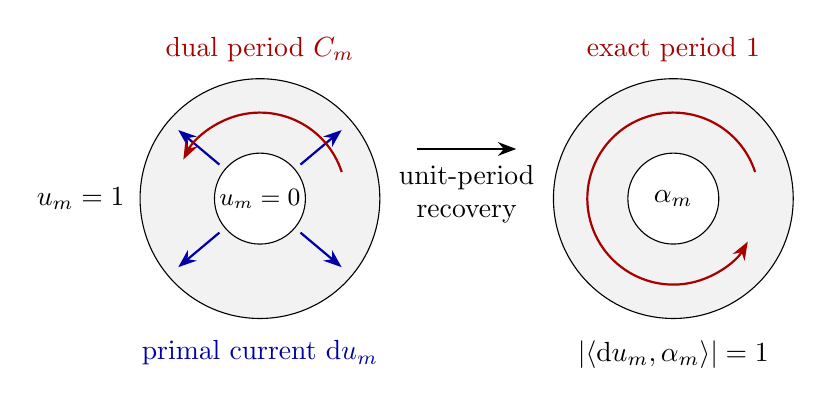
\begin{tikzpicture}[scale=1.05,>=Stealth]
 \fill[gray!10,even odd rule] (0,0) circle (1.45) (0,0) circle (.55);
 \draw (0,0) circle (1.45);
 \draw (0,0) circle (.55);
 \node[font=\small] at (0,0) {$u_m=0$};
 \node[anchor=east] at (-1.52,0) {$u_m=1$};
 \foreach \a in {40,140,220,320}{
   \draw[blue!65!black,->,thick]
       (\a:.64) -- (\a:1.29);
 }
 \draw[red!65!black,->,thick] (18:1.04)
       arc[start angle=18,end angle=153,radius=1.04];
 \node[red!65!black,anchor=south] at (0,1.54)
       {dual period $C_m$};
 \node[blue!65!black,anchor=north] at (0,-1.6)
       {primal current $\dd u_m$};
 \draw[->,thick] (1.9,.6) -- (3.1,.6);
 \node[align=center] at (2.5,.05) {unit-period\\recovery};
 \begin{scope}[xshift=5cm]
  \fill[gray!10,even odd rule] (0,0) circle (1.45) (0,0) circle (.55);
  \draw (0,0) circle (1.45);
  \draw (0,0) circle (.55);
  \draw[red!65!black,->,thick] (18:1.04)
       arc[start angle=18,end angle=330,radius=1.04];
  \node at (0,0) {$\alpha_m$};
  \node[red!65!black,anchor=south] at (0,1.54)
       {exact period $1$};
  \node[anchor=north] at (0,-1.6)
       {$|\langle\dd u_m,\alpha_m\rangle|=1$};
 \end{scope}
\end{tikzpicture}
\caption{The two annular comparisons.  Rotating the condenser current
gives a dual potential with period $C_m$ and hence $\lambda\le1$.
An exact unit-period dual recovery pairs with the unit condenser jump
to give $\lambda\ge1$.  This is a schematic of the test annulus;
the projected discrete graph need not resemble a regular mesh.}
\label{en:fig-reciprocity}
\end{figure}

\begin{lemma}[Rotation of a current]\label{en:current-period}
Rotate the primal current $\dd u_m$ from
Lemma~\ref{en:condenser} to the dual edges, with one consistent crossing
orientation.  In the annulus this is a closed dual cochain with harmonic
local potential branches and period $\pm C_m$.  The branches have
subsequential locally uniform limits with period $\pm\lambda C_0$ and
with total dual relaxed energy at most $\lambda C_0$ over one turn.
\end{lemma}

\begin{proof}
Closedness around a dual face is the primal harmonic equation.
Harmonicity of a potential branch at a dual vertex is the telescoping
sum of $\dd u_m$ around the corresponding primal face.  These identities
count all incidences and are valid also for loops and repeated edges.
The squared dual increments sum to at most $C_m$ on every interior
annular piece.

We justify the existence of branches without assuming regular discrete
annular boundaries.  In a disk with clearance inside the annulus,
arbitrary dual lifts in a smaller disk are connected within the larger
one.  Loops used to integrate the cochain can be filled inside a further
buffer, by Proposition~\ref{inp:topology}; every primal vertex there is
harmonic.  Cellular closedness therefore makes the integral independent
of the chosen path.  On connected overlaps the resulting potentials
differ by constants.

A dual loop with projected winding one can be built along fixed tubes
and closed using small-image joining.  The integer-winding statement of
Proposition~\ref{inp:topology} makes its winding upstairs one, up to the
fixed orientation sign.  Its current integral is the total current
entering one plate, since all intervening primal vertices are harmonic.
Discrete summation by parts gives total current $C_m$: the potential
difference is one and its energy is $C_m$.  Hence the period is
$\pm C_m$.

Normalize branches on a finite overlapping disk cover of any compact
subannulus, propagating constants through chosen overlaps.
In particular, fix a cyclic chain of disks around one positively
oriented circle.  Continue a normalized branch along this chain,
matching on each connected overlap; on returning to the first disk,
the continued branch differs from the original by $\pm C_m$.
Lemma~\ref{en:harmonic-compactness} gives local uniform subsequential
limits.  Their transition constants converge, so their period is
$\pm\lambda C_0$.  Exhausting the annulus yields branches everywhere.
For the energy bound, use disjoint boxes lying in branch disks.  Their
discrete edge energies do not overlap, and their sum is at most $C_m$.
Apply the local lower bound and then exhaust the annulus up to sets of
Lebesgue measure zero.  This gives the asserted bound over one turn.
\end{proof}

Combining Lemmas~\ref{en:scalar} and \ref{en:current-period} with
\eqref{en:period-bound} gives
\begin{equation}\label{en:lambda-upper}
        \lambda C_0\ge
        \lambda\frac{(\lambda C_0)^2}{C_0},
        \qquad\text{hence }\lambda\le1.
\end{equation}
For the reverse inequality, angular recovery must retain its period
before taking any limit.  We record first the measure observation that
makes the gluing sharp.

\begin{lemma}[Energy measures of recovery sequences]\label{en:recovery-measures}
Let $V$ be a bounded patch and let $p$ be smooth on a neighborhood of its
closure.  Choose a recovery sequence on compact sets exhausting $V$
whose total energy tends to $F^*(p,V)$.  Count only edges with both
endpoints in these recovery sets, and put their squared increments
at any of the corresponding projected edge locations.  These measures
converge vaguely in $V$ to $\lambda|\nabla p|^2\,\dd z$.  In particular,
energies weighted by a compactly supported continuous function converge
to the corresponding weighted integral.
\end{lemma}

\begin{proof}
The total masses are bounded.  Let $\nu$ be a subsequential vague limit.
To check its local lower bound, take open sets $W\Subset O\Subset V$
and a compact set $K\subset O$ containing $W$ with a collar.  The energy
tests inside $W$ are eventually counted by the edge measure $\nu_m(K)$.
Lemma~\ref{en:envelope} and compact-set Portmanteau give
\[
 F^*(p,W)\le\liminf_m\nu_m(K)
          \le\limsup_m\nu_m(K)\le\nu(K)\le\nu(O).
\]
Exhaust $O$ by such $W$.  Thus $\nu$ dominates
$\lambda|\nabla p|^2\,\dd z$.  Its total mass is at most the limiting
total recovery energy, which is the total mass of that same measure.
Equality follows.  Every subsequential vague limit is consequently the
stated measure, proving the claim.
\end{proof}

\begin{lemma}[Recovery with exact unit period]\label{en:angular-recovery}
For every sufficiently small $\eta>0$, let
$A_\eta=A(r-\eta,R+\eta)$.  On the dual edges in a neighborhood of the
closed annulus there are closed cochains $\alpha_m$ with exact period
one and
\begin{equation}\label{en:angular-energy}
 \limsup_{m\to\infty}\sum_{e^*\subset A_\eta}|\alpha_m(e^*)|^2
 \le\lambda\left(\frac1{C_0}+o_\eta(1)\right),
             \qquad o_\eta(1)\longrightarrow0.
\end{equation}
The cochains are closed at every cell whose star lies in this
neighborhood; the region can be chosen to contain every edge where
$\dd u_m\ne0$ for all large $m$.
\end{lemma}

\begin{proof}
Take finitely many disks covering a slightly larger closed annulus,
each avoiding the origin, with angle branches
$p_i=\theta_i/(2\pi)$.  Recover $p_i$ uniformly on larger branch disks.
Lemma~\ref{en:recovery-measures} applies to these recoveries, denoted
$v_{i,m}$.  Take a smooth partition of unity $b_i$ with supports compactly
inside the branch disks.  Recover its weights, clip them to be
nonnegative, cut them off in fixed support collars, and normalize their
sum.  This gives $b_{i,m}\to b_i$ uniformly, bounded energies, supports
inside the branch disks, and $\sum_i b_{i,m}=1$ near the annulus.

There is a useful canonical cochain even though its own energy need
not be bounded.  On an oriented dual edge, let
\[
 a_m(e^*)=\frac1{2\pi}\int_{\pi_m(e^*)}\dd\arg z.
\]
Here the integral means the endpoint increment of a continuous argument
lift along the projected edge.  Every sufficiently small edge image
lies in a branch disk, so this is well defined.  Vanishing face mesh
makes $a_m$ closed around every cell under consideration, and its
period around a loop is that loop's projected integer winding.

On the support of $b_{i,m}$ the error
$v_{i,m}-p_i\circ\pi_m$ is a single-valued function tending uniformly
to zero.  Define the globally single-valued error and cochain by
\begin{equation}\label{en:angular-error}
 q_m=\sum_i b_{i,m}(v_{i,m}-p_i\circ\pi_m),
                 \qquad \alpha_m=a_m+\dd q_m.
\end{equation}
The support collars make this definition independent of how terms are
extended by zero.  Since a gradient has zero periods, $\alpha_m$ is
closed and has period exactly one, in the projected orientation.
This conclusion is an identity at each finite resolution.

To bound its energy, apply the discrete product identity on each edge.
On a branch disk, $\dd(p_i\circ\pi_m)=a_m$.  Since the weights sum to
one, the terms containing $a_m$ cancel to give
\[
 \alpha_m(e^*)=
 \sum_i\overline b_{i,m}(e^*)\,\dd v_{i,m}(e^*)
 +\sum_i
 \overline{v_{i,m}-p_i\circ\pi_m}(e^*)\,\dd b_{i,m}(e^*).
\]
The second sum tends to zero in edge $\ell^2$, by uniform convergence
of the errors and bounded energy of the finitely many weights.
Convexity bounds the squared norm of the first sum by the weighted sum
of local recovery energies.  Lemma~\ref{en:recovery-measures} and
$b_{i,m}\to b_i$ turn its limit into
\[
 \lambda\sum_i\int_{A_\eta} b_i|\nabla p_i|^2\,\dd z
 =\lambda\int_{A_\eta}\left|\nabla\frac{\theta}{2\pi}\right|^2\,\dd z
 =\frac{\lambda}{2\pi}\log\frac{R+\eta}{r-\eta}.
\]
One may compute first on a slightly larger closed annulus inside the
cover; its boundary circles have zero limiting energy measure.
The edge averages $\overline b_{i,m}$ converge uniformly to $b_i$ at
the chosen edge locations, by vanishing mesh.  This justifies both
the weighted passage to the limit and restriction to the annulus.
This proves \eqref{en:angular-energy}.  Finally, $u_m$ is constant on
each plate, so its nonzero increments lie in $A_\eta$ eventually by
vanishing edge mesh.  Choosing additional fixed collars gives the
assertion about stars.
\end{proof}

\begin{proposition}[Exact conductance normalization]\label{en:reciprocity}
The scalar in Lemma~\ref{en:scalar} equals one.
\end{proposition}

\begin{proof}
Only $\lambda\ge1$ remains after \eqref{en:lambda-upper}.
Pair $\dd u_m$ with the cochain $\alpha_m$ of
Lemma~\ref{en:angular-recovery}, matching each primal edge with its
crossing dual edge and using the consistent crossing sign.  Then
\begin{equation}\label{en:pairing}
                         \left|\sum_e\dd u_m(e)\alpha_m(e^*)\right|=1.
\end{equation}
To see this at the discrete level, replace $u_m$ by the indicator of the
outer side of an intermediate circle.  Their difference is supported
strictly inside the region of closedness of $\alpha_m$.  Cellular
summation by parts therefore leaves the pairing unchanged.  The
indicator's gradient pairs with $\alpha_m$ along the oriented dual
boundary chain separating the two wells.  This chain has total winding
one up to sign by Proposition~\ref{inp:topology}; the cochain has exact
unit period by \eqref{en:angular-error}.  This proves
\eqref{en:pairing}.  The argument uses the boundary chain with its
multiplicities and does not require a simple discrete plate boundary.

Cauchy--Schwarz, \eqref{en:condenser-limit}, and
\eqref{en:angular-energy} now give
\[
 1\le C_m\sum_{e^*\subset A_\eta}|\alpha_m(e^*)|^2
 \quad\Longrightarrow\quad
 1\le\lambda C_0\,\lambda\left(C_0^{-1}+o_\eta(1)\right).
\]
Let $\eta\downarrow0$.  Thus $1\le\lambda^2$, and
\eqref{en:lambda-upper} proves $\lambda=1$.
\end{proof}

\begin{theorem}[Uniform conformal energy limit]\label{en:variational}
In every coupled extraction and every ordinary chart, both unnormalized
network energies have the same inner relaxed limit:
\begin{equation}\label{en:final-energy}
                   F(u,U)=F^*(u,U)=\int_U|\nabla u|^2\,\dd z
\end{equation}
for every $u\in C(U)\cap W^{1,2}_{\mathrm{loc}}(U)$, with infinite value
when the integral diverges or local Sobolev regularity fails.  The local
uniform lower bounds and recovery conclusions of
Lemma~\ref{en:envelope}, the gluing estimate, and harmonic compactness
hold simultaneously.  In particular, the limiting energy has no
subsequence-dependent multiplicative constant.
\end{theorem}

\begin{proof}
Combine Proposition~\ref{en:representation}, Lemma~\ref{en:scalar}, and
Proposition~\ref{en:reciprocity}.  The preceding construction used the
same countable buffered tests throughout, so its simultaneous and
locality assertions persist.  All arguments apply in every fixed
quantum-unit offset of the extraction.  Their compatibility is the
transport statement of Proposition~\ref{inp:array-interface}.
\end{proof}

\section{From local plane energies to the sphere}\label{sec:sphere}

The energy identification of Section~\ref{sec:energy} was obtained in
ordinary patches of a quantum cone.  We now transfer it to the fixed-area
sphere and include the point at which the contour begins and ends.  The
output is a global variational statement in the same coupling as the
metric-measure convergence.  This common coupling will later allow us to
compare the walks and their metric spaces simultaneously.

Write $\dd A$ for round area on the conformal sphere, and set
\[
 \mathcal D(u)=\int_{S^2}|\nabla u|^2\,\dd A
 \quad\text{for }u\in C(S^2)\cap W^{1,2}(S^2),
\]
with $\mathcal D(u)=+\infty$ for other continuous functions.  The same
notation on an open coordinate domain means the integral over that
domain, with local weak differentiability required.  Conformal
invariance makes these definitions independent of the chosen chart.

\subsection{Transfer on the interior of a contour interval}

First extend the plane conclusion beyond a single ordinary patch.
Retain all forward dyadic unit changes $v=2^k$ from
Proposition~\ref{inp:transport}.  For each fixed $k$, the transformed
rate still tends to infinity, so Theorem~\ref{en:variational} applies
on the ordinary patches inside that cone's normalization disk.
Under the joint zoom \eqref{inp:joint-zoom}, these disks exhaust the
plane away from the cone point.  Pulling the countably many
probability-one conclusions back to the original coordinate proves
the local energy identity everywhere off that point.  Both the
network costs and the two-dimensional Dirichlet integral are unchanged
by these transformations.

For $0<d<1/2$, let $I_d=[d,1-d]$.  The decorated interval surface
associated with the contour on $I_d$ has an interior determined by those
increments.  A compact subset of that interior, together with a small
collar, has all its contour visits strictly inside $I_d$.  Thus its
eventual discrete incidences are read from the internal word; no
information from either omitted end of the tour is needed.  These are
the interval-surface and complete-core assertions used in
Lemma~\ref{inp:complete-core}.

Here is the part of the excursion comparison that permits new
variational observations.  It concerns the joint law of the arrays
and the word, not independence after weak convergence.

\begin{lemma}[Additional observations under excursion conditioning]
\label{sph:block-density}
Fix $0<a<b<1$.  Let $W_N$ be the diffusively rescaled free axial
increment path on $[\lfloor aN\rfloor,\lfloor bN\rfloor]$, with
linear interpolation, and let $Z_N$ be any measurable function of
these increments with values in a fixed compact metrizable space.
Suppose $(W_N,Z_N)\Rightarrow(W,Z)$ along a sequence of even $N$.
There is a nonnegative continuous function $f_{a,b}$ of the limiting
path, with expectation one, such that the corresponding pair under
quadrant-excursion conditioning converges to the law
\[
 f_{a,b}(w)\,\Law(W,Z)(\dd w,\dd z).
\]
In particular, every probability-one property of $(W,Z)$ also
holds for this conditioned limit.  A countable product of
compact-valued observations is allowed for $Z_N$.
\end{lemma}

\begin{proof}
The lemma \emph{Excursion densities} in the spanning-tree sphere
section of \cite{MetricMaps} proves the following statements for
the density $f_N$ of this increment block.  If $w_N\to w$
uniformly, then $f_N(w_N)\to f_{a,b}(w)$; the limit depends
continuously on the two coordinate minima and the net increment.
Moreover, $\sup_N\E[f_N(W_N)^2]<\infty$ under the free law.
These assertions follow there from the entrance-and-exit killed-walk
density and its Gaussian bounds.

Realize the assumed joint convergence almost surely.  For any bounded
continuous test $\Phi$, first truncate the densities at height $K$.
Sequential convergence and bounded convergence give convergence of
the weighted expectations with truncated densities.  The error in
removing truncation is at most
$K^{-1}\|\Phi\|_\infty\sup_N\E[f_N(W_N)^2]$, and the analogous
limit error has the same bound.  Hence
\[
 \E[f_N(W_N)\Phi(W_N,Z_N)]
 \longrightarrow\E[f_{a,b}(W)\Phi(W,Z)].
\]
Taking $\Phi=1$ gives total mass one.  The finite-resolution
change of density depends only on the increment block, so its
weighted expectation is precisely that of the additional block
data under excursion conditioning.  This proves the assertion.
\end{proof}

\begin{proposition}[Energy identification under the sphere conditioning]
\label{sph:transfer}
Consider any joint subsequential extraction of the sphere contour and
the countable internal variational arrays on $I_d$, for every rational
$d\in(0,1/2)$, using the extraction convention of
Proposition~\ref{inp:array-interface}.  Almost surely, on every open
domain compactly contained in the interior of one of these interval
surfaces, both primal and dual inner relaxed energies equal
$\mathcal D$.  This identity holds simultaneously for all continuous
targets, with the value $+\infty$ when the target is not locally
Sobolev or its Dirichlet integral diverges.
\end{proposition}

\begin{proof}
At each resolution retain the energy minima with rational value
constraints and finite unions of relative-time intervals as selectors.
Only increments within $I_d$ enter these internal graphs and tests.
Their compactified values are therefore permissible additional block
data in Lemma~\ref{sph:block-density}.  The corresponding free
experiment is the bilateral sewing at rate $m=2n$.  In that experiment
adjoin these jump-indexed internal tests to the Poisson-instruction
arrays before extraction.  Each added test is computed from its exact
integer increment block and is unchanged when an independent Poisson
clock is attached to the word.  The earlier local identity applies
in this enlarged extraction.  To read it from the internal tests,
use complete pieces and fixed spatial collars as described below.
The vanishing discrepancy of the rescaled clocks only
locates the selectors inside these collars; the numerical energy
outputs themselves are retained unchanged, without a continuity
claim for them under relabeling.

Starting with the given conditioned extraction, take a further
subsequence on which the corresponding free block and its internal
array converge jointly.  This is possible by tightness of the free
contour and compactness of the array space, simultaneously for the
countably many intervals by diagonal extraction.  The weighted-limit
lemma then identifies the already specified conditioned block limit
with the density tilt of this free joint limit.

Theorem~\ref{en:variational} identifies the inner relaxed energies in
that bilateral experiment, away from its distinguished point.  The
distinguished point does not belong to this interval surface:
time zero is almost surely a singleton Brownian contour fiber.
Indeed, each coordinate takes values strictly below its value at zero
arbitrarily close to zero on both sides.  Thus no nontrivial
identification link in either coordinate can have zero as an
endpoint, and neither can the equivalence relation generated by
those links identify zero with another time.  Since $I_d\subset(0,1)$,
its image excludes the distinguished point.

To express the local energy conclusion in terms of the block alone,
reconstruct its abstract decorated interval surface $H_d$ from the
limiting increments using the interval reconstruction in
Proposition~\ref{inp:sewing}.  This reconstruction supplies the surface
and its restricted curve modulo conformal coordinates.  Evaluate
the local identity in a conformal representative, using a countable
atlas and compact exhaustions of its interior; conformal invariance
makes the event independent of that representative.  Both the
restricted curve locating the labels and the coordinate domains for
the targets belong to this reconstructed interval surface.
For a compact $K$ in one such domain and an open enlargement
$U$ with a collar, Lemma~\ref{inp:complete-core} supplies all incidences
near $K$ from the internal word.  The selectors of
Lemma~\ref{inp:sandwich} put every constraint on $K$ between
constraints on internal graphs contained in $U$.  Rational tolerances
and compact exhaustion therefore express the inner relaxed energy
using only the limiting block and its retained arrays.  A change of
the conformal representative preserves both the transported energy
identity and the Dirichlet integral.  The resulting assertion is
intrinsic to $H_d$; the surrounding cone or sphere embedding supplies
no further data for its definition.

The simultaneous quantifier on targets can also be retained in this
transfer.  On a compact coordinate set use a countable dense library
of continuous functions and rational tolerances.  Uniform closeness
of two targets enlarges or shrinks a tolerance constraint by at most
that distance.  The library therefore describes all the relaxed
value tests, jointly measurably in the retained arrays and the target.
This is a discretization of constraints, not an approximation of
Dirichlet energy merely from values on a uniformly dense library.
For varying charts use a countable atlas and compact exhaustions.
The usual Dirichlet integral, with its infinite-value convention,
is likewise Borel on continuous targets: weak derivatives and their
energy can be tested against countably many smooth functions on the
exhaustion.  Existence of a continuous target violating the identity
is consequently an analytic event, obtained by projection from its
Polish function space.  The event of equality for all targets is
universally measurable.  Theorem~\ref{en:variational} gives precisely
this simultaneous event under the free law, so absolute continuity
applies to it without a target-dependent exceptional set.

Absolute continuity of the joint block law now transfers the
probability-one identity to the excursion experiment.  A countable
intersection over $d$, charts, and exhaustions proves the result.
The rest of the sphere contour may be retained in this coupling: the
complement of the event already has zero probability in the internal
marginal, hence also in the joint law.
\end{proof}

The interval interiors exhaust the sphere away from the tour endpoint,
denoted by $p$.  In fact, the inverse image under the continuous contour
of a compact set disjoint from $p$ is compact and avoids times $0$ and
$1$; the same holds after a sufficiently small spatial enlargement.
The interval-surface identification then places the set and its collar
in an interior with $d>0$.  Consequently
Proposition~\ref{sph:transfer} gives the local energy identity at every
point other than $p$.

\subsection{Removing the tour endpoint}

There are two different issues at $p$.  A limit of bounded-energy
functions must have no extra Sobolev singularity there, and recovery
sequences must incur no extra discrete energy there.  The following
elementary fact handles both.

\begin{lemma}[Continuous Sobolev removability]\label{sph:removability}
Let $p$ be a point of a smooth two-dimensional surface.
If $u$ is continuous near $p$, is locally $W^{1,2}$ off $p$, and has
finite Dirichlet integral near $p$, then $u$ is $W^{1,2}$ across $p$.
Moreover, if $u$ is continuous and Sobolev on a compact surface, there
are continuous Sobolev functions $u_r$, constant on a neighborhood of
$p$ and equal to $u$ outside a shrinking disk, such that
\[
 \|u_r-u\|_\infty\longrightarrow0,
 \qquad
 \|u_r-u\|_{W^{1,2}}\longrightarrow0.
\]
\end{lemma}

\begin{proof}
Work in a coordinate disk centered at $p$.  A point has zero
two-dimensional Sobolev capacity: radial logarithmic cutoffs equal to
one on a shrinking inner disk and zero outside a fixed disk have
Dirichlet energies tending to zero.  Testing the weak-derivative
identity off $p$ with the complementary cutoffs proves the identity
across $p$.  More explicitly, the additional term containing the
cutoff gradient tends to zero by Cauchy--Schwarz, since $u$ is bounded
on the support of a fixed smooth test function, while the term
containing $\nabla u$ converges by its local square integrability.

For the approximation choose a smooth cutoff $\chi_r$ equal to one
on $B(p,r)$, zero outside $B(p,2r)$, taking values in $[0,1]$, and
with $\int|\nabla\chi_r|^2\,\dd A\le C$ independently of $r$.
Set
\[
 u_r=u(p)+(1-\chi_r)(u-u(p)).
\]
The uniform error is bounded by the oscillation of $u$ on $B(p,2r)$.
For the gradient error,
\[
 \int|\nabla(u_r-u)|^2\,\dd A
 \le 2\int_{B(p,2r)}|\nabla u|^2\,\dd A
       +2C\sup_{B(p,2r)}|u-u(p)|^2,
\]
and both terms tend to zero.  The ordinary $L^2$ error follows from
uniform convergence.
\end{proof}

In a coupled extraction, choose a location $\pi_n(v)\in S^2$ for each
primal vertex from one of its contour visits; different choices have
uniformly vanishing discrepancy.  Use $\pi_n^*$ on the dual.
For functions on the varying vertex sets, uniform convergence to $u$
means
\[
 \max_{v\in V_n}|u_n(v)-u(\pi_n(v))|\longrightarrow0.
\]
The small-image joining and mesh assertions in the input guarantee that
this convention agrees with the local comparisons already used.
Harmonicity on an open set $U$ means that the graph Laplacian vanishes
at every vertex whose location is in $U$.  For a compact subset of
$U$, all adjoining stars also lie in $U$ once $n$ is large; thus
this convention permits the buffered uses of
Lemma~\ref{en:harmonic-compactness}.

\begin{theorem}[Global sphere energies]\label{sph:energy}
From any subsequence of the tree-decorated sphere maps, one can take a
further joint extraction and a coupling with the limiting ordinary
quantum sphere such that the following statements hold almost surely.
\begin{enumerate}
\item If $u_n$ converges uniformly to $u\in C(S^2)$, then
\[
 \liminf_{n\to\infty}\en_n(u_n)\ge\mathcal D(u).
\]
\item For each $u\in C(S^2)\cap W^{1,2}(S^2)$ there are uniformly
convergent approximations $u_n$ for which
\[
 \en_n(u_n)\longrightarrow\mathcal D(u).
\]
Both assertions hold on the dual with $\en_n^*$ and $\pi_n^*$.
\item On every open set, graph-harmonic functions with bounded energy
and bounded absolute value are locally equicontinuous under these
locations and have locally uniformly convergent subsequences.  This
holds also on the dual and at the tour endpoint.
\end{enumerate}
All these conclusions may be required in the same extraction as the
metric and measure comparison below.
\end{theorem}

\begin{proof}
Retain the internal tests of Proposition~\ref{sph:transfer} and also
the whole-sphere tests defining uniform relaxed energy.  The latter
are countable compactified arrays; they need no local conditional
kernel.  The selector sandwich applies to them in the same way.

Suppose first that $\liminf_n\en_n(u_n)<\infty$ and pass to a subsequence
realizing this liminf.  On disjoint compact-interior patches away from
$p$, Proposition~\ref{sph:transfer} bounds their limiting Dirichlet
integrals by the discrete energies in those patches.  Exhausting the
complement of $p$ gives
\[
 \int_{S^2\setminus\{p\}}|\nabla u|^2\,\dd A
 \le\liminf_n\en_n(u_n).
\]
Lemma~\ref{sph:removability} supplies the weak derivative at $p$.
This proves the first assertion, including its infinite-value case.

For the upper bound, first take a continuous Sobolev target that is
constant near $p$.  Cover the complement of a smaller constant disk
by finitely many patches from Proposition~\ref{sph:transfer}.
Subdivide it into finitely many smaller coordinate regions with
piecewise smooth boundaries, each contained in one patch, and thicken
these regions slightly.  The boundaries have zero round area, so
their collars can be chosen with arbitrarily small total integral
of $|\nabla u|^2$.  Local recovery on the thickened regions and
successive applications of Lemma~\ref{en:fundamental} now give
recovery on the compact complement: the main energy is bounded by
the sum of the target energies on those regions, and only the
chosen small collars are counted more than once.  The error terms
from gluing tend to zero by uniform agreement on each fixed
collar.  This proves recovery with arbitrarily small energy slack.
Extend by the constant on the
smaller disk.  To make the extension exact, use a cutoff whose
transition lies in a fixed annulus where the target is constant.
Apply the finite-cover recovery just proved to a slightly larger
annular neighborhood and a smooth cutoff $b$ that is constant on
its two collars.  If $b_n$ is its recovery and
$\delta_n>\|b_n-b\|_\infty$ tends to zero, replace $b_n$ by
\[
 \left(\frac{b_n-\delta_n}{1-2\delta_n}\right)\vee0\wedge1.
\]
This is exactly zero and one on the respective flat collars, and
its energy is at most $(1-2\delta_n)^{-2}\en_n(b_n)$.
The functions being joined differ by $o(1)$
on the transition, so the extra term in the gluing estimate is $o(1)$.
The mesh tends to zero, hence every edge crossing either gluing
boundary is contained in the fixed collar for all sufficiently large
$n$.

For a general continuous Sobolev $u$, apply the approximation
$u_r$ of Lemma~\ref{sph:removability}.  Recover each fixed $u_r$ first,
then use a diagonal choice of $r\downarrow0$.  Uniform convergence and
convergence of $\mathcal D(u_r)$ give the desired upper bound; the
first assertion makes it an equality.  The proof for the dual is
identical.

Away from $p$, harmonic compactness follows from
Lemma~\ref{en:harmonic-compactness}.  To include $p$, take any fixed
finite stack of disjoint annuli centered at $p$, each of the same
aspect ratio, in a domain of harmonicity.  Every transition annulus
avoids $p$.  By the preceding local recovery, its dual cutoff can
be taken with energy bounded by a constant depending only on the
aspect ratio, with exact constant values on its two sides.  Fill
the inner side by the constant; this uses only a flat collar in the
annulus.  Lemma~\ref{en:circuit} gives a primal circuit in each annulus
whose oscillation squared is bounded by that constant times the
primal energy in the annulus.  Among $k$ disjoint annuli, one
therefore has oscillation at most $C k^{-1/2}$ when the total energy
is bounded.  The maximum principle transfers this oscillation to
all vertices inside its circuit.  First choose $k$, and then take
large $n$; no annulus radius depends on $n$.  Finite covers give
equicontinuity, and bounded values give compactness.  Exchanging
primal and dual proves the remaining assertion.
\end{proof}

\subsection{Keeping the metric and the quantum area in the same coupling}

The coordinate used for energy convergence must also describe the
metric-measure limit.  The contour correspondence makes this precise.

\begin{proposition}[Joint spatial comparison]\label{sph:comparison}
The extraction in Theorem~\ref{sph:energy} can be chosen so that its
limiting sphere is the one in the metric-measure limit and, almost
surely,
\begin{align}
 \sup_{v,w\in V_n}
 \big|a_n d_n(v,w)-D_h(\pi_n(v),\pi_n(w))\big|&\longrightarrow0,
 \label{sph:distortion}\\
 \sup_{x\in S^2}\dist_{D_h}(x,\pi_n(V_n))&\longrightarrow0,
 \label{sph:dense}\\
 (\pi_n)_*\mu_n&\Longrightarrow\mu_h.
 \label{sph:measure}
\end{align}
The maximum round diameter of a projected edge tends to zero.
The measure $\mu_h$ is nonatomic and has full support, and $D_h$
induces the round topology.
\end{proposition}

\begin{proof}
The sphere-identification proposition and the final normalization
argument for spanning-tree maps in \cite{MetricMaps} give, jointly
with the excursion, the contour correspondence
\[
 \bigl\{(v_{\lfloor2nt\rfloor},\eta(t)):0\le t\le1\bigr\}
\]
with distortion tending to zero.  Here $v_j$ is the primal vertex
at the start of tour step $j$ and $\eta$ is the sphere contour.
Those results identify the metric of this very peanosphere limit;
they do not introduce an independent quantum sphere.  Their
deterministic diameter normalization is the $a_n$ in
Theorem~\ref{thm:main}.  Choosing one visit for each vertex changes
the correspondence by a uniformly vanishing discrepancy, which
gives \eqref{sph:distortion} and \eqref{sph:dense}.

There are $2n$ tour step starts.  Their vertex occupation measure is
$\mu_n$: horizontal tree traversals are counted at their starting
vertices, and vertical steps count the non-tree half-edges at their
incident vertices.  Every half-edge is counted once, including both
half-edges of a loop.  The area parameterization of $\eta$ therefore
gives \eqref{sph:measure}.  Mesh convergence is the sphere
projection construction preceding Proposition~\ref{inp:topology}.
Nonatomicity, full support, and agreement of the metric and conformal
topologies are the quantum-area and metric properties in the same
repository input.

All these variables may be retained together with the compactified
energy arrays before extraction.  The metric identification is
unchanged upon a further extraction, so it holds in the coupling of
Theorem~\ref{sph:energy}.
\end{proof}

\section{A Green estimate in the finite map law}
\label{sec:green}

Uniform approximation of energies concerns continuous functions.  To
control the walk clock, we also need to show that bounded sources of
small stationary mass have small potentials.  We prove this directly
under the finite map law.  The argument combines a spanning-forest
formula for the inverse Laplacian with the two tree contours in
Mullin's encoding.

Write $N=2n$.  Let $H_n$ be the positive graph Laplacian on $V_n$,
using counting measure and unit conductances, so that
\[
 \langle u,H_nu\rangle=\en_n(u)
       =\sum_{ab\in E(M_n)}(u(a)-u(b))^2.
\]
There is one term for each unoriented edge, and loops contribute zero.
For a real function $f$ with $\mu_n(f)=0$, define $G_nf$ by
\begin{equation}\label{gr:green-definition}
 H_nG_nf=\mu_n f,
 \qquad \mu_n(G_nf)=0.
\end{equation}
Here $\mu_nf$ on the right denotes the vector with entry
$\mu_n(v)f(v)$ at $v$.  Connectedness gives existence and uniqueness.

\begin{proposition}[Small-mass Green estimate]
\label{gr:green-bound}
For each fixed $\rho\in(0,1/2)$ there are nonnegative random variables
$A_n$, measurable functions of $M_n$, such that
\begin{equation}\label{gr:green-main}
 \sup_{n\geq1}\E A_n<\infty,
 \qquad
 \|G_nf\|_\infty\leq A_n\,\mu_n(|f|)^\rho
\end{equation}
simultaneously for all real functions $f:V_n\to\R$ satisfying
$\|f\|_\infty\leq1$ and $\mu_n(f)=0$.
The expectation is under the map marginal of the uniform rooted
map--spanning-tree pair law.  In particular, $(A_n)$ is tight.
\end{proposition}

We first identify the exact inverse formula.  We then estimate its
terms by grouping tree cuts according to the amount of tour time on
their smaller side.

\subsection{The inverse Laplacian as a sum over cuts}

The next identity is a consequence of the matrix-tree theorem and
its forest expansions; see the all-minors theorem of \cite{Chaiken}
and \cite[Chapter~4]{LP} for electrical networks and spanning trees.
We give the determinant argument to specify the multiplicities and
centering used here.

\begin{lemma}[Forest representation]
\label{gr:forest}
Let $\mathcal G$ be a finite connected multigraph, with positive
probability measure $\mu$ on its vertex set $V$, and let $H$ be its
unit-conductance graph Laplacian.  Suppose $q:V\to\R$ satisfies
$\sum_{v\in V}q(v)=0$, and let $u$ solve
$Hu=q$, $\mu(u)=0$.  For a uniform spanning tree $T$ of $\mathcal G$
and an edge $e\in T$, choose either component $S_e$ of $T\setminus e$,
and let $b_e$ be the number of graph edges between $S_e$ and
$V\setminus S_e$, with multiplicity.  Then
\begin{equation}\label{gr:forest-identity}
 u(x)=\E_T\sum_{e\in T}
       \frac{q(S_e)\bigl(\1_{\{x\in S_e\}}-\mu(S_e)\bigr)}{b_e},
 \qquad x\in V,
\end{equation}
where $q(S)=\sum_{v\in S}q(v)$.  The value does not depend on the
choice of component for any $e$.
\end{lemma}

\begin{proof}
The one-vertex case is immediate, so suppose $m:=|V|\geq2$.
Orient the non-loop edges arbitrarily and delete the row of a fixed
vertex $o$ from the incidence matrix.  Denote the resulting matrix by
$B$, and write $\widehat q$ for $q$ with its $o$-coordinate deleted.
The reduced Laplacian is $\widehat H=BB^{\mathsf T}$.  If $\tau$ is
the number of spanning trees, the matrix-tree theorem and the
determinant lemma give
\begin{equation}\label{gr:rank-one}
 \det(\widehat H+z\widehat q\widehat q^{\mathsf T})
       =\tau\bigl(1+z\widehat q^{\mathsf T}
                            \widehat H^{-1}\widehat q\bigr).
\end{equation}
For $z\geq0$, apply Cauchy--Binet to the matrix obtained by appending
$\sqrt z\widehat q$ to $B$.  A term contributing to the coefficient
of $z$ selects $m-2$ incidence columns and the source column.
The incidence columns are independent exactly when their edges form
a spanning forest with two components.  Indeed, a cycle gives a
linear dependence, whereas an acyclic graph with $m-2$ edges has
exactly two components, counting isolated vertices.

For such a forest $F$, let $S_F$ be its component not containing $o$.
Its corresponding determinant has absolute value $|q(S_F)|$.
To see this, successively eliminate leaf rows and their incident
forest columns.  Eliminating a leaf adds its source entry to its
neighbor's entry.  The component containing $o$ disappears into the
deleted row, and the last entry in the other component is
$\sum_{v\in S_F}q(v)$.  Consequently, comparison of the coefficients
of $z$ in \eqref{gr:rank-one} yields
\begin{equation}\label{gr:two-forest-quadratic}
 \widehat q^{\mathsf T}\widehat H^{-1}\widehat q
       =\frac1\tau\sum_F q(S_F)^2.
\end{equation}

Let $H^+$ be the inverse of $H$ on counting-mean-zero vectors,
extended by zero on constants.  Solving the equation with value zero
at $o$ shows that the left side of
\eqref{gr:two-forest-quadratic} equals $q^{\mathsf T}H^+q$.
Polarization therefore gives, for any two vectors $q,r$ of total
sum zero,
\begin{equation}\label{gr:two-forest-bilinear}
 q^{\mathsf T}H^+r=\frac1\tau\sum_F q(S_F)r(S_F).
\end{equation}
Replacing $S_F$ by its complement changes the sign of each factor,
so the product is independent of this choice.

Every two-component forest $F$ has exactly $b(F)$ extensions to a
spanning tree: add any one of the graph edges across its cut.
Thus, when all pairs $(T,e)$ are counted, $F=T\setminus e$ occurs
exactly $b(F)$ times.  This explains the denominator in
\eqref{gr:forest-identity}.  Apply \eqref{gr:two-forest-bilinear}
with $r=\delta_x-\mu$.  Its left side is
\[
 (H^+q)(x)-\mu(H^+q)=u(x),
\]
and its right side, regrouped by $(T,e)$, is the asserted expression.
Loops enter neither the reduced incidence matrix nor a cut; parallel
edges are counted separately throughout.
\end{proof}

\subsection{What a tree cut records in the tour}

We use the finite form of Mullin's correspondence \cite{Mullin}, with
the incidence conventions of \cite[Section~``Independent-walk encoding
and local quantum surfaces'']{MetricMaps}.  The $N$ steps form a
quadrant excursion whose horizontal and vertical coordinates are
denoted by $L$ and $R$.  Horizontal steps traverse the selected
primal tree $T$; vertical steps traverse the complementary dual tree
$T^*$.  In each coordinate an up-step is matched with the down-step
that first returns to its initial height.  A matched horizontal pair
represents a tree edge.  A matched vertical pair represents a
non-tree map edge between the primal vertices at its two step starts.
Let $v_i$ be the primal vertex at step start $i$, with all indices
read cyclically modulo $N$.

\begin{lemma}[Tour mass and cut size]
\label{gr:tour-cut}
For each $v\in V_n$,
\begin{equation}\label{gr:tour-degree}
 \#\{0\leq i<N:v_i=v\}=\deg_{M_n}(v).
\end{equation}
For $e\in T$, the step starts visiting either component of
$T\setminus e$ form a cyclic interval.  Choose a component $S_e$
whose interval $I_e$ has length $\ell_e\leq N/2$.  If the lengths
agree, choose the component not containing $v_0$.  Then
\begin{equation}\label{gr:tour-cut-identities}
 \mu_n(S_e)=\frac{\ell_e}{N},
 \qquad b_e=1+D_e^*,
\end{equation}
where $D_e^*$ is the distance in $T^*$ between the dual vertices at
the two horizontal traversal steps of $e$.
\end{lemma}

\begin{proof}
Associate each step start with the departing step.  The two
horizontal traversals of a tree edge depart once from each endpoint,
and hence count its two incidences.  The two steps of a vertical
matched pair count the two incidences of its non-tree edge.  When
that edge is a loop, both are assigned to the same vertex.
Every step belongs to one such pair, proving
\eqref{gr:tour-degree}; this is also the tour-measure lemma of
\cite[Section~``From tree excursions to the measured quantum
sphere'']{MetricMaps}.

The primal vertex changes only along horizontal steps.  It passes
between the two components of $T\setminus e$ exactly at the two
traversals of $e$.  Thus each side occupies one cyclic interval, and
\eqref{gr:tour-degree} proves the mass identity.

There is exactly one tree edge across this cut, namely $e$.
A non-tree edge crosses it precisely when exactly one step of its
vertical matched pair belongs to $I_e$.  Ignore horizontal holds
and follow the resulting dual-tree contour segment.  An edge of
$T^*$ is traversed once on this segment exactly when its matched
steps lie on opposite sides of $I_e$; every other dual edge is
traversed zero or twice.  In a tree the edges traversed an odd number
of times by a path are exactly the edges on the simple path between
its endpoints.  These endpoints are the dual vertices at the two
horizontal traversals of $e$, since horizontal steps do not change
the dual vertex.  There are therefore $D_e^*$ non-tree edges across
the cut, giving $b_e=1+D_e^*$.
\end{proof}

Hereafter expectations involving both $T$ and the map use the uniform
pair law.  The sequence $(v_i)$ is determined by the horizontal
contour and the locations of the horizontal slots.  Thus the cut
intervals, their lengths, and the smaller-side convention in
Lemma~\ref{gr:tour-cut} are determined without inspecting the shape
of the vertical contour.  By \eqref{gr:tour-degree}, the same is true
of the vertex masses.

The conditional structure of the finite law is useful.  Let $J$
be the number of horizontal steps.  Conditional on $J$, the horizontal
slots form a uniform $J$-subset of $\{0,\ldots,N-1\}$.  Conditional
on these slots, the two coordinate strings, with holds deleted, are
independent uniform Dyck excursions of lengths $J$ and $N-J$.
In fact, writing $C_k=(k+1)^{-1}\binom{2k}{k}$ for the Catalan
numbers, the number of quadrant excursions with $J=2k$ is
\begin{equation}\label{gr:schedule-count}
 \binom{2n}{2k}C_kC_{n-k},
 \qquad
 \sum_{k=0}^n\binom{2n}{2k}C_kC_{n-k}=C_nC_{n+1}.
\end{equation}
The last equality is Vandermonde's identity after writing out the
Catalan numbers.  These counts also prove the stated conditional
independence.  Catalan estimates and a binomial tail bound give
absolute $C,c>0$ such that
\begin{equation}\label{gr:count-tail}
 \P\{J\notin[N/4,3N/4]\}\leq C(N+1)^3e^{-cN}.
\end{equation}
The same schedule calculation is recorded in the excursion discussion
of \cite[Section~``From tree excursions to the measured quantum
sphere'']{MetricMaps}.  It is an exact calculation in the fixed-size
law.

\subsection{Distances in a uniform contour tree}

The cut denominator in \eqref{gr:tour-cut-identities} is a dual-tree
distance.  The next estimates quantify its typical size and also
control how many primal cuts can surround a given tour time.

\begin{lemma}[Contour distance estimates]
\label{gr:dyck}
Let $\mathcal T_s$ be a uniform rooted plane tree with $s/2$ edges,
where $s\geq2$ is even, and write $w_i$, $i\in\Z/s\Z$, for its
cyclic contour vertices.  If $i,j$ are deterministic with
$0\leq j\leq s$, set
\[
 D=\dist_{\mathcal T_s}(w_i,w_{i+j}),
 \qquad d=1+\min(j,s-j).
\]
There are absolute constants $C,c>0$ such that, for every integer
$a\geq0$,
\begin{equation}\label{gr:dyck-density}
 \P(D=a)\leq C(a+1)^2d^{-3/2}e^{-ca^2/d}.
\end{equation}
Consequently, for every fixed $p>0$,
\begin{equation}\label{gr:dyck-moments}
 \|(1+D)^{-1}\|_{L^2}\leq C d^{-1/2},
 \qquad \|D\|_{L^p}\leq C_p\sqrt d.
\end{equation}
For every deterministic cyclic segment $K$ from corner $i$ through
corner $i+L$, where $1\leq L\leq s$,
\begin{equation}\label{gr:contour-diameter}
 \bigl\|\diam_{\mathcal T_s}\{w_{i+r}:0\leq r\leq L\}\bigr\|_{L^4}
       \leq C\sqrt L.
\end{equation}
\end{lemma}

\begin{proof}
Rerooting a plane tree at its $i$th contour corner is a bijection on
rooted plane trees with $s/2$ edges.  Its inverse reroots by $s-i$
corners.  Thus the rerooted tree is uniform, and $D$ has the law of
the height at time $j$ of a uniform Dyck excursion of length $s$.

Let $p_l(a)$ be the probability that a simple symmetric walk started
at zero stays nonnegative for $l$ steps and finishes at $a$.
Reflection and the binomial estimate give
\begin{align}
 p_l(a)
 &=2^{-l}\left[
       \binom{l}{(l+a)/2}-\binom{l}{(l+a+2)/2}\right],
       \label{gr:killed-kernel}\\
 p_l(a)&\leq C(a+1)(l+1)^{-3/2}
                         e^{-ca^2/(l+1)},\nonumber
\end{align}
with inadmissible binomial coefficients interpreted as zero.
For even $s$, $p_s(0)$ is comparable to $(s+1)^{-3/2}$.
The Markov property and time reversal of the second segment give
\[
 \P(D=a)=\frac{p_j(a)p_{s-j}(a)}{p_s(0)}.
\]
Inserting \eqref{gr:killed-kernel} proves
\eqref{gr:dyck-density}.  Summing it after multiplication by
$(a+1)^{-2}$ or by $a^p$ proves
\eqref{gr:dyck-moments}.  In the first case the remaining Gaussian
sum is at most $C\sqrt d$, so the second moment is at most $C/d$.

For completeness, the diameter estimate follows by dyadic chaining.
Reroot at the deterministic first corner of $K$ and parametrize its
steps by the integers in $[0,L]$.  At refinement level $l$, use the
times $\lfloor kL/2^l\rfloor$, $0\leq k\leq2^l$, and stop at
$l=\lceil\log_2L\rceil$.  These grids are nested and the last one
contains every integer in $[0,L]$.  Include the initial increment
from $0$ to $L$.  For $l\geq1$, there are $O(2^l)$ new-to-parent
increments at level $l$, each spanning at most $C L2^{-l}$ steps.
By the fourth-moment estimate and
$\|\max_k Z_k\|_{L^4}^4\leq\sum_k\|Z_k\|_{L^4}^4$, the maximum
tree distance across these increments has $L^4$ norm at most
\[
 C2^{l/4}\sqrt{L2^{-l}}=C\sqrt L\,2^{-l/4}.
\]
Every contour vertex can be joined to the first vertex through its
ancestors in the dyadic grids.  The triangle inequality and the
summability of $2^{-l/4}$ bound the maximum distance from that first
vertex by $C\sqrt L$ in $L^4$.  The diameter is at most twice this
maximum.  For $L=1$ the bound follows directly from the single edge.
\end{proof}

\subsection{The sum of reciprocal cut sizes at one scale}

For a dyadic integer $M$ with $1\leq M\leq N/2$, let
\[
 \mathcal E_M=\{e\in T:M\leq\ell_e<2M\},
 \qquad
 U_{M,t}=\sum_{\substack{e\in\mathcal E_M\\t\in I_e}}\frac1{b_e},
 \qquad t\in\Z/N\Z.
\]
The intervals in this sum come from the horizontal tree.  Their
denominators are governed by the independent vertical tree once the
schedule and the horizontal tree have been fixed.

\begin{lemma}[One-scale estimate]
\label{gr:one-scale}
There is an absolute constant $C$ such that, for every $n$, every
dyadic $M\leq N/2$, and every deterministic tour time $t$,
\begin{equation}\label{gr:Ut}
 \E U_{M,t}^2\leq C.
\end{equation}
\end{lemma}

\begin{proof}
First condition on a count $J\in[N/4,3N/4]$.  Consider all cyclic
intervals containing $t$ whose lengths lie in $[M,2M)$ and are at
most $N/2$.  There are at most $C(M+1)^2$ such intervals.  For each
one, a uniform schedule puts at least $c_0M$ vertical steps in both
the interval and its complement, except with probability
$Ce^{-cM}$, for suitable absolute $c_0,c>0$.  Indeed, the vertical
density is at least $1/4$, both sets have at least $M$ slots, and
the hypergeometric lower-tail bound applies.  Taking a union bound,
let $\mathcal B_{M,t}$ be the event that this property fails for
some interval.  Uniformly over the balanced counts,
\begin{equation}\label{gr:schedule-tail}
 \P(\mathcal B_{M,t}\mid J)
       \leq C(M+1)^2e^{-cM}.
\end{equation}

Fix a schedule outside $\mathcal B_{M,t}$ and then condition on the
horizontal Dyck excursion.  This fixes all intervals in $U_{M,t}$.
For each one, its dual endpoints are separated in the vertical
contour by the number $j$ of vertical steps in that interval.
Both $j$ and $(N-J)-j$ are at least $c_0M$.  Lemmas
\ref{gr:tour-cut} and \ref{gr:dyck}, followed by the triangle
inequality in $L^2$ of the remaining vertical excursion, imply
\begin{equation}\label{gr:vertical-bound}
 \|U_{M,t}\|_{L^2(R\mid\text{schedule},L)}
       \leq\frac{C}{\sqrt M}\,K_{M,t},
 \qquad
 K_{M,t}:=\#\{e\in\mathcal E_M:t\in I_e\}.
\end{equation}

We next bound this number of horizontal cuts.  Any two components
$S_e,S_{e'}$ containing $v_t$ are nested unless their union is all
of $V_n$.  This elementary tree property follows by considering
the components cut off from $v_t$: they are either nested or
disjoint.  The union alternative cannot occur for the chosen
smaller sides, since
\[
 \mu_n(S_e\cup S_{e'})
 =\mu_n(S_e)+\mu_n(S_{e'})-\mu_n(S_e\cap S_{e'})<1.
\]
Here each of the first two terms is at most $1/2$, and the
intersection contains $v_t$, whose mass is positive.
Thus all components counted by $K_{M,t}$ are nested.

If the family is nonempty, let $S$ be its largest component and
choose a contour vertex immediately outside its interval.  It has
a representative at cyclic distance at most $2M+2$ from $t$.
The tree path from $v_t$ to that vertex crosses all $K_{M,t}$ cut
edges.  Hence $K_{M,t}$ is at most the diameter of the horizontal
contour image of the deterministic window of tour times within
$2M+2$ of $t$.  After the schedule has been fixed and holds deleted,
this is a deterministic contour segment with at most $4M+4$
horizontal steps.  If the window covers the entire tour, the full
horizontal contour instead has length $J\leq N\leq4M+4$.
A segment with no horizontal steps has diameter zero; otherwise
Lemma~\ref{gr:dyck} applies.  Uniformly in the schedule, we obtain
\begin{equation}\label{gr:horizontal-count}
 \E\bigl[K_{M,t}^2\mid\text{schedule}\bigr]\leq CM.
\end{equation}
Combining \eqref{gr:vertical-bound} and
\eqref{gr:horizontal-count} proves the required bound on schedules
outside $\mathcal B_{M,t}$ with balanced counts.

For the exceptional schedules, use a deterministic bound.
Every interval counted by $K_{M,t}$ has its two delimiting tree
traversals within cyclic distance $2M+2$ of $t$.  Distinct tree
edges have distinct traversal occurrences, so
$K_{M,t}\leq C(M+1)$.  Since $b_e\geq1$, the same bound holds
for $U_{M,t}$.  By \eqref{gr:schedule-tail}, the contribution of
these schedules to its second moment is at most
$C(M+1)^4e^{-cM}$, uniformly bounded in $M$.
Finally, $U_{M,t}\leq N$ always.  The unbalanced counts contribute
at most $CN^2(N+1)^3e^{-cN}$ by \eqref{gr:count-tail}, also
uniformly bounded.  This proves \eqref{gr:Ut} under the full law.
\end{proof}

\subsection{Summing the scales}

We now return to the inverse formula.  Lemma~\ref{gr:one-scale}
controls the cut sum at a fixed time; a grid converts this into a
uniform bound over vertices.

\begin{proof}[Proof of Proposition~\ref{gr:green-bound}]
The one-vertex case has $G_nf=0$, so set $A_n=0$ there.  Otherwise,
for each dyadic $M\leq N/2$, choose a deterministic cyclic grid
$\Gamma_M$.  For $M\geq8$, take its gaps at most $M/4$, its
cardinality at most $CN/M$, and its distinct points separated by
at least $cM$.  For $M<8$, use all step indices; the same
cardinality and separation bounds hold with absolute constants.

An interval of length in $[M,2M)$ containing a fixed time $t$
contains a grid point within cyclic distance $2M$ of $t$.  There
are only a bounded number of grid points in this neighborhood.
Consequently,
\begin{equation}\label{gr:grid-comparison}
 \sup_t U_{M,t}\leq C\max_{t\in\Gamma_M}U_{M,t}.
\end{equation}
Every visit to a given vertex belongs to the same side of a tree
cut.  Also, counting the visits in each interval gives
\[
 \sum_{e\in\mathcal E_M}\frac{\mu_n(S_e)}{b_e}
       =\frac1N\sum_{t=0}^{N-1}U_{M,t}.
\]
It follows that
\begin{align}
 W_M&:=\sup_{x\in V_n}\sum_{e\in\mathcal E_M}
        \frac{\1_{\{x\in S_e\}}+\mu_n(S_e)}{b_e}
       \leq C\max_{t\in\Gamma_M}U_{M,t},
          \label{gr:WM}\\
 \E W_M&\leq C\left(\sum_{t\in\Gamma_M}
                                    \E U_{M,t}^2\right)^{1/2}
       \leq C\sqrt{N/M}.\label{gr:WM-mean}
\end{align}
No independence among the grid variables is needed here.

Fix $f$ as in the proposition and write $m_f=\mu_n(|f|)$.
For $e\in\mathcal E_M$, the source mass obeys
\begin{equation}\label{gr:source-interpolation}
 \left|\sum_{v\in S_e}\mu_n(v)f(v)\right|
 \leq\min(2M/N,m_f)
 \leq(2M/N)^{1-\rho}m_f^\rho.
\end{equation}
Define, for the realized pair $(M_n,T)$,
\[
 Y_n(M_n,T)=\sum_{\substack{M\leq N/2\\M\text{ dyadic}}}
                   (2M/N)^{1-\rho}W_M.
\]
By \eqref{gr:WM-mean},
\begin{equation}\label{gr:Y-mean}
 \E Y_n\leq C_\rho
       \sum_{\substack{M\leq N/2\\M\text{ dyadic}}}
                        (M/N)^{1/2-\rho}
       \leq C_\rho.
\end{equation}
The last bound is a geometric sum, using $\rho<1/2$.

Conditional on $M_n$, the selected tree is uniform.  Define
\begin{equation}\label{gr:An}
 A_n(M_n)=\E\bigl[Y_n(M_n,T)\mid M_n\bigr].
\end{equation}
Apply Lemma~\ref{gr:forest} with $q=\mu_nf$.  Taking absolute
values, grouping by $M$, and using
\eqref{gr:source-interpolation} proves
\[
 \|G_nf\|_\infty\leq A_n(M_n)m_f^\rho.
\]
The variable in \eqref{gr:An} is independent of the choice of $f$,
so this bound holds simultaneously for all admissible functions.
The tower property and \eqref{gr:Y-mean} give
$\sup_n\E A_n<\infty$, and Markov's inequality gives tightness.
\end{proof}

The estimate depends only on the finite map law and its spanning
trees.  In particular, it controls the full potential of a small
source, including any behavior on vertex sets that uniform
approximation of continuous functions might fail to detect.

\section{Resolvents and conditional path laws}\label{sec:dynamics}

Uniform convergence of energies concerns continuous functions, whereas
the speed measure may be singular with respect to round area.  The
Green estimate bridges this difference: it makes a bounded source on
a set of small quantum mass produce a uniformly small potential.
After removing that potential, a resolvent is locally harmonic, so
the compactness theorem for harmonic functions applies.  We first
give this argument for a deterministic sequence of graphs.  The last
subsection applies it in the coupled random environments and proves
Theorem~\ref{thm:main}.

\subsection{A deterministic convergence criterion}

Let $S^2$ carry its round distance $d_0$ and area $\dd A$.  Let $\mu$
be a nonatomic probability measure with full support.  Suppose the
quadratic form
\begin{equation}\label{dyn:continuum-form}
 \cE(u,u)=\frac12\int_{S^2}|\nabla u|^2\,\dd A,
 \qquad u\in C^\infty(S^2),
\end{equation}
is closable in $L^2(\mu)$, and its closure $(\cE,\mathcal F)$ is a
regular conservative Dirichlet form with an associated continuous-path
diffusion $B$.  We always start $B$ with law $\mu$.  These hypotheses
hold for the Liouville area measures used here; the time-change and
Dirichlet-form constructions are treated in
\cite{GRV,Berestycki}, with general form theory in \cite{FOT}.
Our normalization is the explicit factor $1/2$ in
\eqref{dyn:continuum-form}.

For each $n$, let $\mathcal G_n$ be a finite connected graph, allowing loops and
multiple edges, with vertex set $V_n$ and a strictly positive
probability measure $\mu_n$ on $V_n$.  Write
\[
 (H_nu)(v)=\sum_{vw}\bigl(u(v)-u(w)\bigr),
 \qquad
 \en_n(u)=\sum_{\{v,w\}}(u(v)-u(w))^2.
\]
The first sum counts incidences at $v$, and the second counts
unoriented edges with multiplicity.  Loop summands vanish.
Let $Y^n$ be the chain with generator
\begin{equation}\label{dyn:abstract-generator}
 (\mathcal L_nu)(v)=-\frac{(H_nu)(v)}{2\mu_n(v)}.
\end{equation}
It is reversible with respect to $\mu_n$, and its form is
$\cE_n(u,u)=\en_n(u)/2$.  Choose maps $\pi_n:V_n\to S^2$.
Uniform comparison of functions always means
\[
 \|u_n-u\circ\pi_n\|_{\infty,V_n}\longrightarrow0.
\]
No injectivity of $\pi_n$ is required.

\begin{theorem}[From energies and Green bounds to path laws]
\label{dyn:conditional}
In the deterministic setting just defined, assume the following.
\begin{enumerate}[label=\textup{(\roman*)}]
\item $(\pi_n)_*\mu_n\Rightarrow\mu$, and the maximum projected
edge length tends to zero:
\[
 \max_{\{v,w\}\in E(\mathcal G_n)}d_0(\pi_n(v),\pi_n(w))\longrightarrow0.
\]
\item Every uniformly convergent sequence with continuous limit $u$
satisfies
\[
 \liminf_n\en_n(u_n)\ge\int|\nabla u|^2\,\dd A,
\]
where the right side is $+\infty$ unless $u\in W^{1,2}(S^2)$.
Every smooth $u$ has a uniformly convergent recovery sequence with
energy tending to that integral.
\item For every open $U\subset S^2$, sequences that are graph-harmonic
at all vertices in $\pi_n^{-1}(U)$ and have uniformly bounded
supremum and total energy are locally equicontinuous in $U$ under
$\pi_n$, and locally uniformly precompact there.
Here equicontinuity means that, for every compact $K\subset U$,
\[
 \lim_{\delta\downarrow0}\limsup_n
 \sup_{\substack{\pi_n(v),\pi_n(w)\in K\\
                  d_0(\pi_n(v),\pi_n(w))\le\delta}}
       |u_n(v)-u_n(w)|=0,
\]
and precompactness means uniform comparison with a continuous
function on each compact subset after a common subsequence.
\item For the centered solution operator
\[
 H_nG_ng=\mu_n g,\qquad \mu_n(G_ng)=0,
 \qquad \mu_n(g)=0,
\]
there are constants $C<\infty$ and $\rho>0$, independent of $n$, such
that
\begin{equation}\label{dyn:green-assumption}
 \|G_ng\|_\infty\le C\,\mu_n(|g|)^\rho
 \quad\text{if }\|g\|_\infty\le1\text{ and }\mu_n(g)=0.
\end{equation}
\end{enumerate}
Then the laws of $(\pi_n(Y^n_t))_{0\le t\le T}$, with initial law
$\mu_n$, converge in $D([0,T],S^2)$ to the law of
$(B_t)_{0\le t\le T}$, for every finite $T$.  The limit has continuous
paths.  In addition, for every $\alpha>0$ and $f\in C(S^2)$, the
resolvents converge uniformly under $\pi_n$.
\end{theorem}

We prove the theorem through four lemmas.  Their hypotheses throughout
are those of Theorem~\ref{dyn:conditional}.  Notice that full support
and weak convergence of the measures already imply that $\pi_n(V_n)$
becomes dense: otherwise a fixed open ball of positive $\mu$-mass
would be missed along a subsequence.

\begin{lemma}[Continuous Sobolev functions in the closed form]
\label{dyn:smooth-core}
If $u\in C(S^2)\cap W^{1,2}(S^2)$, then $u\in\mathcal F$ and its
closed-form energy is the right side of
\eqref{dyn:continuum-form}.  It has smooth approximations converging
both uniformly and in the form norm.  Two continuous versions of
the same element of $L^2(\mu)$ are equal everywhere.
\end{lemma}

\begin{proof}
In coordinate disks, mollification of a continuous Sobolev function
converges both uniformly on smaller disks and in Sobolev norm.
A smooth partition of unity gives smooth functions $u_j$ on the
sphere with these two convergences globally.  Since $\mu$ is finite,
uniform convergence also gives $L^2(\mu)$ convergence.  Thus $(u_j)$
is Cauchy for $\cE(\cdot,\cdot)+\|\cdot\|_{L^2(\mu)}^2$ and has
limit $u$ in the stipulated closure.  The gradient convergence
identifies its energy.  Polarization gives the same identity for
the bilinear form on continuous Sobolev functions.  Finally a
nonzero continuous difference is bounded away from zero on some
open set, which has positive $\mu$-mass by full support.
\end{proof}

Let $R^n_\alpha=(\alpha-\mathcal L_n)^{-1}$, and let $R_\alpha$ be the
$L^2(\mu)$ resolvent of $(\cE,\mathcal F)$.

\begin{lemma}[Uniform resolvent convergence]\label{dyn:resolvent}
For every $\alpha>0$ and $f\in C(S^2)$, $R_\alpha f$ has a unique
continuous version, which belongs to round $W^{1,2}$, and
\begin{equation}\label{dyn:resolvent-limit}
 \bigl\|R^n_\alpha(f\circ\pi_n)
              -(R_\alpha f)\circ\pi_n\bigr\|_\infty
       \longrightarrow0.
\end{equation}
The same conclusion holds with right-hand sides $f_n$ converging
uniformly under $\pi_n$ to $f$.
\end{lemma}

\begin{proof}
Put $u_n=R^n_\alpha(f\circ\pi_n)$.  The maximum principle and the
resolvent equation give
\begin{equation}\label{dyn:resolvent-bounds}
 \|u_n\|_\infty\le\frac{\|f\|_\infty}{\alpha},
 \qquad
 H_nu_n=\mu_n g_n,
 \qquad
 g_n=2(f\circ\pi_n-\alpha u_n).
\end{equation}
In particular $g_n$ is uniformly bounded, and multiplying the equation
by $u_n$ shows that $\en_n(u_n)$ is uniformly bounded.

We first prove equicontinuity.  Fix a point $x\in S^2$, and choose
disjoint open neighborhoods $U$ of $x$ and $V$ of a different point.
Take $\mu$-null boundaries, with $\mu(V)>0$.  The neighborhood $U$
may be made arbitrarily small in $\mu$-mass because $\mu$ has no
atoms.  Write $U_n=\pi_n^{-1}(U)$ and $V_n'=\pi_n^{-1}(V)$, and set
\[
 q_n=g_n\1_{U_n}
       -\frac{\mu_n(g_n\1_{U_n})}{\mu_n(V_n')}\1_{V_n'}.
\]
For large $n$, the denominator is bounded below.  Hence $q_n$ has
mean zero, bounded supremum, and
$\mu_n(|q_n|)\le C_1\mu_n(U_n)$.  Scaling
\eqref{dyn:green-assumption} yields
\[
 \|G_nq_n\|_\infty\le C_2\mu_n(U_n)^\rho.
\]
Also
\[
 \en_n(G_nq_n)=\mu_n((G_nq_n)q_n)
 \le\|G_nq_n\|_\infty\mu_n(|q_n|).
\]
Thus $u_n-G_nq_n$ has bounded energy and supremum and is harmonic
on $U_n$.  Hypothesis~(iii) makes this difference equicontinuous on
compact subsets of $U$.  Given an oscillation tolerance, first
choose $U$ so that $G_nq_n$ has smaller supremum, and then use
harmonic equicontinuity inside $U$.  A finite cover of $S^2$ proves
equicontinuity of the original sequence.  Boundedness and density of
$\pi_n(V_n)$ now give uniformly convergent subsequences.

Let $u$ be one such limit.  Hypothesis~(ii) and
Lemma~\ref{dyn:smooth-core} show that $u\in\mathcal F\cap C(S^2)$.
The discrete resolvent minimizes
\[
 J_n(v)=\frac12\en_n(v)+\alpha\mu_n(v^2)
                       -2\mu_n((f\circ\pi_n)v).
\]
The energy lower bound, uniform convergence, and weak convergence of
the measures imply
\[
 \cE(u,u)+\alpha\mu(u^2)-2\mu(fu)
       \le\liminf_n J_n(u_n).
\]
For any smooth $v$, take its uniform recovery sequence $v_n$.
Minimality gives $J_n(u_n)\le J_n(v_n)$, and the latter converges to
$\cE(v,v)+\alpha\mu(v^2)-2\mu(fv)$.  Smooth functions are a core
of the closed form by its definition, so $u$ minimizes this
functional over all of $\mathcal F$.  Strict convexity for $\alpha>0$
identifies $u=R_\alpha f$ in $L^2(\mu)$.  Full support makes its
continuous version unique.  Every subsequence has the same limit,
which proves \eqref{dyn:resolvent-limit}.

Finally, $\|R^n_\alpha a-R^n_\alpha b\|_\infty
\le\alpha^{-1}\|a-b\|_\infty$.  This contraction bound proves the
claim for varying right-hand sides.
\end{proof}

\subsection{Controlling small time intervals}

Resolvent convergence integrates the walk over time.  To recover
the actual clock, we next construct functions that separate spatial
sets and whose discrete generators are bounded.  The needed continuum
approximation is uniform, rather than merely in $L^2(\mu)$.

\begin{lemma}[Uniform resolvent approximation]\label{dyn:feller}
For every $f\in C(S^2)$,
\begin{equation}\label{dyn:approximate-identity}
 \|\alpha R_\alpha f-f\|_\infty\longrightarrow0
 \qquad\text{as }\alpha\longrightarrow\infty.
\end{equation}
\end{lemma}

\begin{proof}
First suppose $f$ is smooth, and put $w_\alpha=\alpha R_\alpha f$.
The spectral theorem for the nonnegative self-adjoint form operator
gives $w_\alpha\to f$ in the form norm.  Indeed the spectral
multiplier $\alpha/(\alpha+\lambda)$ tends to one and is bounded by
one, so dominated convergence applies with spectral weight
$1+\lambda$.  By Lemma~\ref{dyn:smooth-core},
\[
 \|\nabla(w_\alpha-f)\|_{L^2(\dd A)}\longrightarrow0.
\]
The maximum principle, or its discrete version followed by
Lemma~\ref{dyn:resolvent}, gives
\begin{equation}\label{dyn:range}
 \min f\le w_\alpha\le\max f.
\end{equation}

We also need convergence in round $L^2$, which does not follow by
changing the measure in the form norm.  Let $c_\alpha$ be the round
average of $w_\alpha-f$.  Round Poincare gives
\[
 \|w_\alpha-f-c_\alpha\|_{L^2(\dd A)}\longrightarrow0.
\]
The constants $c_\alpha$ are bounded by \eqref{dyn:range}.  If a
subsequence has limit $c$, then $w_\alpha\to f+c$ in round $L^2$
on that subsequence, and therefore along a further subsequence almost
everywhere.  Consequently
$\min f\le f+c\le\max f$ almost everywhere for round area.
Continuity of $f$ makes its essential extrema equal to its extrema:
every neighborhood of a minimizer or maximizer has positive round
area.  The two inequalities force $c\ge0$ and $c\le0$.
Thus $c=0$, and $w_\alpha-f\to0$ in round $W^{1,2}$.

Fix a small coordinate disk about a point $x$, and a fixed annulus
inside that disk surrounding a smaller neighborhood of $x$.
Radial averaging of the round $W^{1,2}$ error supplies, for each
large $\alpha$, a circle in this annulus on which the trace of
$w_\alpha-f$ tends to zero in one-dimensional $H^1$.  The radii stay
in a fixed compact subinterval of $(0,\infty)$, so the
one-dimensional Sobolev inequality gives uniform convergence on
these circles.  Almost every radius has the Sobolev trace of the
continuous representative, which is the trace we choose.

Let $D_\alpha$ be the disk inside the chosen circle.  The resolvent
equation is
\begin{equation}\label{dyn:weak-resolvent}
 \cE(w_\alpha,v)+\alpha\int(w_\alpha-f)v\,\dd\mu=0,
 \qquad v\in\mathcal F.
\end{equation}
Choose a constant $K$ strictly above the boundary values of
$w_\alpha$ and at least $\sup_{D_\alpha} f$.
The positive part $(w_\alpha-K)^+$ on $D_\alpha$, extended by zero,
vanishes in a collar of the circle and is continuous Sobolev.
Lemma~\ref{dyn:smooth-core} makes it an admissible test in
\eqref{dyn:weak-resolvent}.  The two terms are nonnegative; the
second is at least $\alpha\int ((w_\alpha-K)^+)^2\,\dd\mu$.
Thus $w_\alpha\le K$ on the disk, first $\mu$-almost everywhere and
then everywhere by continuity and full support.  The negative-part
test gives the lower bound.  Letting the strict slack tend to zero
shows that the values inside the circle are bounded by its boundary
values and the extrema of $f$ in the disk.

The oscillation of $f$ on sufficiently small disks is arbitrarily
small.  The boundary convergence and this comparison therefore
give uniform convergence on a neighborhood of $x$.  A finite cover
proves \eqref{dyn:approximate-identity} for smooth $f$.
For continuous $f$, approximate it uniformly by a smooth function
and use the contraction $\|\alpha R_\alpha\|_{\infty\to\infty}\le1$.
\end{proof}

\begin{lemma}[An exit estimate uniform over starting vertices]
\label{dyn:tightness}
For $d>0$ and $v\in V_n$, let
\[
 \tau^n_d(v)=\inf\{t\ge0:
   d_0(\pi_n(Y^n_t),\pi_n(v))\ge d\}.
\]
Then
\begin{equation}\label{dyn:exit}
 \lim_{s\downarrow0}\limsup_{n\to\infty}
       \sup_{v\in V_n}\P_v[\tau^n_d(v)\le s]=0.
\end{equation}
The stationary projected path laws are tight in $D([0,T],S^2)$,
and all their limits are supported on continuous paths.
\end{lemma}

\begin{proof}
Cover the sphere by finitely many round disks of radius less than
$d/8$.  For each choose a smooth function $f$ in $[0,1]$, zero on
that disk, and one outside the concentric disk of radius $d/2$.
If $\pi_n(v)$ is in the smaller disk and displacement from
$\pi_n(v)$ reaches $d$, the value of $f$ at the new location is one.

Fix $b>0$.  Lemmas~\ref{dyn:feller} and \ref{dyn:resolvent}, first
with a sufficiently large fixed $\alpha$ and then with sufficiently
large $n$, give for each of this finite family a function
\[
 v_n=\alpha R^n_\alpha(f\circ\pi_n),\qquad
 \|v_n-f\circ\pi_n\|_\infty\le b.
\]
Its generator satisfies
\[
 \mathcal L_nv_n=\alpha(v_n-f\circ\pi_n),
 \qquad \|\mathcal L_nv_n\|_\infty\le C_b,
\]
with a common $C_b$ for the finite family and all sufficiently large
$n$.  Start the chain at $v$ in the corresponding small disk and
stop at $\sigma=\tau^n_d(v)\wedge s$.  If
$p=\P_v[\tau^n_d(v)\le s]$, then
\[
 \E_v[v_n(Y^n_\sigma)]\ge p-b,
 \qquad
 \E_v[v_n(Y^n_\sigma)]
   =v_n(v)+\E_v\int_0^\sigma \mathcal L_nv_n(Y^n_t)\,\dd t
   \le b+C_bs.
\]
Hence $p\le2b+C_bs$, uniformly over all starting vertices.
First let $s\downarrow0$ and then $b\downarrow0$ to obtain
\eqref{dyn:exit}.

Apply the strong Markov property to the chain $Y^n$ after any
stopping time.  Since \eqref{dyn:exit} is uniform over its current
vertex, it gives the usual stopping-time increment condition for
the projected paths.  The projection itself need not be Markov.
Apply Aldous's stopping-time criterion \cite{Aldous} to the three
coordinate functions of the round sphere in $\R^3$; their values
are bounded.  This gives tightness of each coordinate path law.
The largest coordinate jump is bounded by the maximum projected
edge length, which tends to zero.  Under $J_1$ convergence any jump
of a limit is approximated by jumps of the approximating paths,
so every coordinate limit is continuous.  Coordinate tightness
with continuous limits gives joint tightness with continuous
limits in $\R^3$: on continuous limits, $J_1$ convergence agrees
with uniform convergence, allowing a common time comparison for
the three coordinates.  The limits remain in the closed set
$S^2$, proving the assertion.
\end{proof}

\subsection{Identifying the entire conditional law}

\begin{proof}[Completion of the proof of Theorem~\ref{dyn:conditional}]
Take a subsequence of the stationary projected path laws with a weak
limit.  By Lemma~\ref{dyn:tightness}, diagonal extraction on the
horizons $1,2,\ldots$ gives a consistent continuous-path law on
$[0,\infty)$, denoted by $Q$.  Restrictions are consistent because
the limits are continuous at the restriction times.

Let $f_0,\ldots,f_k\in C(S^2)$ and $\alpha_1,\ldots,\alpha_k>0$.
Integrate the stationary finite-dimensional expectation at times
$0,t_1,t_1+t_2,\ldots,t_1+\cdots+t_k$ against
$\prod_{j=1}^k e^{-\alpha_jt_j}\,\dd t_j$.  The Markov property
and the resolvent identity give exactly
\begin{equation}\label{dyn:laplace}
 \mu_n\!\left[
  (f_0\circ\pi_n)R^n_{\alpha_1}
  \left((f_1\circ\pi_n)R^n_{\alpha_2}
    \left(\cdots(f_{k-1}\circ\pi_n)
                R^n_{\alpha_k}(f_k\circ\pi_n)\cdots\right)\right)
 \right].
\end{equation}
Successive applications of Lemma~\ref{dyn:resolvent}, including its
varying-data assertion, and weak convergence of the measures show
that \eqref{dyn:laplace} converges to
\[
 \mu\!\left[f_0R_{\alpha_1}
       \left(f_1R_{\alpha_2}
          \left(\cdots f_{k-1}R_{\alpha_k}f_k\cdots\right)\right)
       \right].
\]
By the semigroup-resolvent relation for the closed form, this is the
same integrated expectation for the stationary diffusion $B$.

It is also the integrated expectation for $Q$.  On bounded time
boxes this follows from weak path convergence, since evaluation at
fixed times is continuous at continuous paths.  Dominated
convergence then integrates over the gaps.  The contribution of
the complement of a large time box is bounded uniformly by the
tails of the product of exponentials, times
$\prod_j\|f_j\|_\infty$.

The product expectations under $Q$ and under $B$ are bounded
continuous functions of $(t_1,\ldots,t_k)$, including zero gaps.
Uniqueness of multivariate Laplace transforms makes these
functions equal: one may apply one-dimensional uniqueness
successively in each coordinate, and then use continuity to
remove almost-everywhere qualifications.  Product tests determine
probability measures on the compact product $(S^2)^{k+1}$.
Thus $Q$ and the law of $B$ have the same finite-dimensional
distributions, and hence the same law on continuous paths.
Every subsequential limit is the same, proving the theorem.
\end{proof}

\subsection{The clock and the metric-space conclusion}

We now return to the random maps.  The exact relation between the
graph energy and the prescribed walk fixes the clock without any
subsequence-dependent factor.

\begin{lemma}[Exact energy of the accelerated walk]\label{dyn:energy-clock}
For the half-edge walk of Theorem~\ref{thm:main},
\[
 -\langle u,nL_nu\rangle_{L^2(\mu_n)}=\frac12\en_n(u).
\]
Equivalently, $nL_n=-\tfrac12\mu_n^{-1}H_n$, where
$\mu_n^{-1}$ denotes division by vertex mass.
\end{lemma}

\begin{proof}
The generator convention gives $H_n=-\deg\,L_n$.  Since
$\mu_n(v)=\deg(v)/(2n)$,
\[
 -\sum_v\mu_n(v)u(v)nL_nu(v)
   =\frac12\sum_vu(v)H_nu(v)
   =\frac12\sum_{\{v,w\}}(u(v)-u(w))^2.
\]
Loops contribute zero to both sides.  Their degree contributions
are already included in the first identity, so no holding-time
correction is needed.
\end{proof}

\begin{proof}[Proof of Theorem~\ref{thm:main}]\label{dyn:main-proof}
Start with any subsequence.  Retain the random variable $A_n$ of
Proposition~\ref{gr:green-bound} together with all the contour,
spatial, and local and whole-sphere array variables used in
Theorem~\ref{sph:energy} and Proposition~\ref{sph:comparison}.
Its uniform first-moment bound gives tightness, so these variables
admit a joint further extraction.  Apply the sphere results to this
enlarged extraction and use a Skorokhod representation.  On the
resulting probability-one event, their conclusions hold and $A_n$
converges to a finite random variable.  In particular
$\sup_n A_n<\infty$ after discarding finitely many initial terms.

Fix a realization in this probability-one event.  Its limiting
quantum sphere is now a fixed measured conformal sphere.  The
projections $\pi_n$, measures, edge mesh, uniform energy bounds and
recovery, and harmonic compactness satisfy hypotheses~(i)--(iii)
of Theorem~\ref{dyn:conditional}.  The realized bounded $A_n$ gives
hypothesis~(iv).  The Liouville form is exactly
\eqref{dyn:continuum-form} with $\mu=\mu_h$.  By
Lemma~\ref{dyn:energy-clock}, the chain in that deterministic theorem
is $Y^n_t=X^n_{nt}$.  Consequently its conditional projected path
law converges to the conditional law of $B^h$, for every fixed
finite horizon.  All probabilities in this invocation are taken
on the individual fixed graphs.  The random object being compared
is the conditional probability law itself.

It remains to express this comparison in the metric $\delta_T$.
The round topology and the $D_h$ topology agree on the compact
limiting sphere, so the identity map between them is uniformly
continuous in both directions.  The path-law convergence just
proved therefore also holds in $D([0,T],(S^2,D_h))$.

The correspondences in Proposition~\ref{sph:comparison} have
distortions tending to zero.  The standard correspondence gluing
constructs a common metric space containing isometric copies of
all $(V_n,a_nd_n)$ and $(S^2,D_h)$, with
\[
 \sup_{v\in V_n}\dist_Z\bigl(v,\pi_n(v)\bigr)\longrightarrow0.
\]
For completeness, for each $n$ attach its copy to the sphere by
cross-distances obtained by taking the infimum over corresponding
pairs, adding numbers $\varepsilon_n\downarrow0$ larger than half
the respective distortions;
use the shortest-path metric on the union, identifying only the
common sphere, and then take the completion.  This preserves the
metrics of every copy.  The images become close in Hausdorff
distance, and their measures become close in Prokhorov distance.

Apply the embedding to each coordinate of a chain path.  Its
distance in the common Skorokhod space from its $\pi_n$-projected
path is bounded by the displayed supremum, using the identity time
change.  The corresponding probability laws therefore have
Prokhorov distance tending to zero.  Combining this with the
projected law convergence shows that all three terms defining
$\delta_T$ tend to zero in the coupled extraction.

We have obtained almost-sure convergence in a further coupling from
every original subsequence, to the prescribed quantum sphere and
its conditional diffusion law.  The subsequence principle gives
convergence in distribution through all positive integers $n$.
Forgetting the root, the spanning tree, and the contour marks
leaves precisely the states in Theorem~\ref{thm:main}.  The same
choice $c=1$ works for every time horizon.
\end{proof}

\begin{thebibliography}{99}

\bibitem{Aldous}
D. Aldous,
\emph{Stopping times and tightness},
Ann. Probab. \textbf{6} (1978), no.~2, 335--340.
\href{https://doi.org/10.1214/aop/1176995579}{doi:10.1214/aop/1176995579}.

\bibitem{Berestycki}
N. Berestycki,
\emph{Diffusion in planar Liouville quantum gravity},
Ann. Inst. Henri Poincar\'e Probab. Stat. \textbf{51} (2015), no.~3,
947--964.
\href{https://doi.org/10.1214/14-AIHP605}{doi:10.1214/14-AIHP605}.

\bibitem{BG}
N. Berestycki and E. Gwynne,
\emph{Random walks on mated-CRT planar maps and Liouville Brownian motion},
Comm. Math. Phys. \textbf{395} (2022), no.~2, 773--857.
\href{https://doi.org/10.1007/s00220-022-04482-y}{doi:10.1007/s00220-022-04482-y}.
\href{https://arxiv.org/abs/2003.10320v2}{arXiv:2003.10320v2}.

\bibitem{Chaiken}
S. Chaiken,
\emph{A combinatorial proof of the all minors matrix tree theorem},
SIAM J. Algebraic Discrete Methods \textbf{3} (1982), no.~3, 319--329.
\href{https://doi.org/10.1137/0603033}{doi:10.1137/0603033}.

\bibitem{DMS}
B. Duplantier, J. Miller, and S. Sheffield,
\emph{Liouville quantum gravity as a mating of trees},
Ast\'erisque \textbf{427} (2021), viii+258 pp.
\href{https://doi.org/10.24033/ast.1149}{doi:10.24033/ast.1149}.
\href{https://arxiv.org/abs/1409.7055v4}{arXiv:1409.7055v4}.

\bibitem{Dykhne}
A. M. Dykhne,
\emph{Conductivity of a two-dimensional two-phase system},
Soviet Phys. JETP \textbf{32} (1971), no.~1, 63--65;
translated from Zh. Eksp. Teor. Fiz. \textbf{59} (1970), 110--115.

\bibitem{FOT}
M. Fukushima, Y. Oshima, and M. Takeda,
\emph{Dirichlet Forms and Symmetric Markov Processes},
second revised and extended edition,
De Gruyter Studies in Mathematics, vol.~19,
Walter de Gruyter, Berlin, 2011.
\href{https://doi.org/10.1515/9783110218091}{doi:10.1515/9783110218091}.

\bibitem{GRV}
C. Garban, R. Rhodes, and V. Vargas,
\emph{Liouville Brownian motion},
Ann. Probab. \textbf{44} (2016), no.~4, 3076--3110.
\href{https://doi.org/10.1214/15-AOP1042}{doi:10.1214/15-AOP1042}.

\bibitem{GRVForm}
C. Garban, R. Rhodes, and V. Vargas,
\emph{On the heat kernel and the Dirichlet form of Liouville Brownian motion},
Electron. J. Probab. \textbf{19} (2014), Paper No.~96, 1--25.
\href{https://doi.org/10.1214/EJP.v19-2950}{doi:10.1214/EJP.v19-2950}.

\bibitem{GHS}
E. Gwynne, N. Holden, and X. Sun,
\emph{A mating-of-trees approach for graph distances in random planar maps},
Probab. Theory Related Fields \textbf{177} (2020), nos.~3--4, 1043--1102.
\href{https://doi.org/10.1007/s00440-020-00969-8}{doi:10.1007/s00440-020-00969-8}.

\bibitem{GMMetric}
E. Gwynne and J. Miller,
\emph{Existence and uniqueness of the Liouville quantum gravity metric
for $\gamma\in(0,2)$},
Invent. Math. \textbf{223} (2021), no.~1, 213--333.
\href{https://doi.org/10.1007/s00222-020-00991-6}{doi:10.1007/s00222-020-00991-6}.

\bibitem{GMConformal}
E. Gwynne and J. Miller,
\emph{Conformal covariance of the Liouville quantum gravity metric
for $\gamma\in(0,2)$},
Ann. Inst. Henri Poincar\'e Probab. Stat. \textbf{57} (2021), no.~2,
1016--1031.
\href{https://doi.org/10.1214/20-AIHP1105}{doi:10.1214/20-AIHP1105}.

\bibitem{GM}
E. Gwynne and J. Miller,
\emph{Random walk on random planar maps: spectral dimension, resistance
and displacement},
Ann. Probab. \textbf{49} (2021), no.~3, 1097--1128.
\href{https://doi.org/10.1214/20-AOP1471}{doi:10.1214/20-AOP1471}.

\bibitem{GMSHarmonic}
E. Gwynne, J. Miller, and S. Sheffield,
\emph{Harmonic functions on mated-CRT maps},
Electron. J. Probab. \textbf{24} (2019), Paper No.~58, 1--55.
\href{https://doi.org/10.1214/19-EJP325}{doi:10.1214/19-EJP325}.

\bibitem{GMS}
E. Gwynne, J. Miller, and S. Sheffield,
\emph{The Tutte embedding of the mated-CRT map converges to Liouville
quantum gravity},
Ann. Probab. \textbf{49} (2021), no.~4, 1677--1717.
\href{https://doi.org/10.1214/20-AOP1487}{doi:10.1214/20-AOP1487}.

\bibitem{GMS2}
E. Gwynne, J. Miller, and S. Sheffield,
\emph{An invariance principle for ergodic scale-free random environments},
Acta Math. \textbf{228} (2022), no.~2, 303--384.
\href{https://doi.org/10.4310/ACTA.2022.v228.n2.a2}{doi:10.4310/ACTA.2022.v228.n2.a2}.

\bibitem{LP}
R. Lyons and Y. Peres,
\emph{Probability on Trees and Networks},
Cambridge Series in Statistical and Probabilistic Mathematics, vol.~42,
Cambridge University Press, New York, 2016.
\href{https://doi.org/10.1017/9781316672815}{doi:10.1017/9781316672815}.

\bibitem{IG4}
J. Miller and S. Sheffield,
\emph{Imaginary geometry IV: interior rays, whole-plane reversibility,
and space-filling trees},
Probab. Theory Related Fields \textbf{169} (2017), nos.~3--4, 729--869.
\href{https://doi.org/10.1007/s00440-017-0780-2}{doi:10.1007/s00440-017-0780-2}.
\href{https://arxiv.org/abs/1302.4738v2}{arXiv:1302.4738v2}.

\bibitem{MSSphere}
J. Miller and S. Sheffield,
\emph{Liouville quantum gravity spheres as matings of finite-diameter trees},
Ann. Inst. Henri Poincar\'e Probab. Stat. \textbf{55} (2019), no.~3,
1712--1750.
\href{https://doi.org/10.1214/18-AIHP932}{doi:10.1214/18-AIHP932}.
\href{https://arxiv.org/abs/1506.03804v4}{arXiv:1506.03804v4}.

\bibitem{Mullin}
R. C. Mullin,
\emph{On the enumeration of tree-rooted maps},
Canad. J. Math. \textbf{19} (1967), 174--183.
\href{https://doi.org/10.4153/CJM-1967-010-x}{doi:10.4153/CJM-1967-010-x}.

\bibitem{ConformalMaps}
OpenAI,
\emph{Canonical conformal limits of subcritical FK planar maps},
OpenAI Math Release preprint
\href{https://github.com/openai/math/blob/main/preprints/Canonical-conformal-limits-of-subcritical-FK-planar-maps-September-24-2026/main.pdf}{OAI:Canonical-conformal-limits-of-subcritical-FK-planar-maps-September-24-2026},
2026.

\bibitem{MetricMaps}
OpenAI,
\emph{Metric-measure limits of subcritical FK and spanning-tree planar maps},
OpenAI Math Release preprint
\href{https://github.com/openai/math/blob/main/preprints/Metric-measure-limits-of-subcritical-FK-and-spanning-tree-planar-maps-September-24-2026/main.pdf}{OAI:Metric-measure-limits-of-subcritical-FK-and-spanning-tree-planar-maps-September-24-2026},
2026.

\end{thebibliography}

\end{document}
